\documentclass{article}
\usepackage{graphicx} % Required for inserting images
\usepackage{wrapfig}
\usepackage{geometry}
\usepackage{tikz}
\usetikzlibrary{shapes, arrows}
\usepackage{pgf-pie}
\usepackage[backend=bibtex,style=alphabetic,sorting=ynt]{biblatex}
\usepackage[sharp]{easylist}
\usepackage[simplified]{pgf-umlcd}
\usepackage{lscape}

\usepackage[T1]{fontenc}
\usepackage{inconsolata}
\usepackage{color}
\definecolor{bluekeywords}{rgb}{0.13,0.13,1}
\definecolor{greencomments}{rgb}{0,0.5,0}
\definecolor{redstrings}{rgb}{0.9,0,0}
\usepackage{listings}
\lstset{language=[Sharp]C,
  showspaces=false,
  showtabs=false,
  breaklines=true,
  showstringspaces=false,
  breakatwhitespace=true,
  escapeinside={(*@}{@*)},
  commentstyle=\color{greencomments},
  keywordstyle=\color{bluekeywords},
  stringstyle=\color{redstrings},
  basicstyle=\ttfamily
}

\tikzstyle{startstop} = [rectangle, rounded corners, minimum width=3cm, minimum height=1cm,text centered, draw=black, fill=red!30]
\tikzstyle{io} = [trapezium, trapezium left angle=70, trapezium right angle=110, minimum width=3cm, minimum height=1cm, text centered, draw=black, fill=blue!30]
\tikzstyle{process} = [rectangle, minimum width=3cm, minimum height=1cm, text centered, draw=black, fill=orange!30]
\tikzstyle{decision} = [diamond, minimum width=3cm, minimum height=1cm, text centered, draw=black, fill=green!30]
\tikzstyle{arrow} = [thick,->,>=stealth]
%https://www.overleaf.com/learn/latex/LaTeX_Graphics_using_TikZ%3A_A_Tutorial_for_Beginners_(Part_3)%E2%80%94Creating_Flowcharts
%For decomposition diagram
\definecolor{rootcol}{HTML}{576490}
\definecolor{l1col}{HTML}{23C9FF}
\definecolor{l2col}{HTML}{7CC6FE}
\definecolor{l3col}{HTML}{CCD5FF}
\definecolor{l4col}{HTML}{E7BBE3}
\tikzstyle{root} = [rectangle, rounded corners, minimum width=3cm, minimum height=0.8cm, text centered, draw=black, fill=rootcol]
\tikzstyle{l1} = [rectangle, rounded corners, minimum width=3cm, minimum height=0.8cm, text centered, draw=black, fill=l1col]
\tikzstyle{l2} = [rectangle, rounded corners, minimum width=3cm, minimum height=0.8cm, text centered, draw=black, fill=l2col]
\tikzstyle{l3} = [rectangle, rounded corners, minimum width=3cm, minimum height=0.8cm, text centered, draw=black, fill=l3col]
\tikzstyle{l4} = [rectangle, rounded corners, minimum width=3cm, minimum height=0.8cm, text centered, draw=black, fill=l4col]

\bibliography{biblio}
\geometry{
a4paper,
total = {170mm,257mm},
left = 20mm,
top = 20mm,
}
\setlength{\parindent}{0pt}
\graphicspath{ {./Images/} }

\newcommand{\parBr}{\vspace{5mm}}%5mm vertical space
\newcommand{\myparagraph}[1]{\paragraph{#1}\mbox{}\\} %line break after paragraph declared
\newcommand{\smallBr}{\vspace{1.5mm}}
\newcommand{\mycomment}[1]{}

\begin{document}
\title{Computer Science \\ Advanced GCE H447 \\ Unit F453 \\[2\baselineskip]}
\author{\large Name: Karol Jeziorczak \\ Candidate Number: 4162 \\ Centre Name: Rugby High School \\ Centre Number: 31255 }
\date{}
\maketitle
\newpage
\tableofcontents
\newpage
\listoffigures
\newpage

\section{Abstract}
I decided to create a game for my coursework. I had researched the market to influence my game to make it more appealing to the target audience. Creating the game was very challenging and challenged my  limited understanding of c\#, and forced me to learn the language in greater detail, it also challenged the methods that I tend to favour when approaching a challenge forcing me to explore new ways of computational methods. I decided on a 2D rouge-like game with a heavy focus on melee combat and movement. For this I needed to make a character controller, dungeon generation algorithm, enemy AI and balanced items for the player. Each requiring it's own delicate calibration to make the game fun. 

\section{Introduction}
For my project I intend to create a 2D rouge like game which is focuses on melee combat. This game would be like Rain World with Celeste movement. I chose this style because there are few games which focus on melee combat and this would help it stand out amongst the other games, the rouge like aspect would allow every run to be unique and distinct. Allowing people to replay the game multiple times without getting bored.

\parBr

The melee combat will be close range and it will allow people to play in distinctive styles, for example people will be able to change their weapon and ability to suit the play style that they are looking for, making any play style viable.

\parBr

There will be progress through floors. When the player completes one floor they can move on and enter the next floor. At the end of each floor there will be a boss that the player must defeat to progress.

\parBr

The loot and map generation will be random meaning that the player cannot memorize the layout and do the same thing every time but need to adjust to the environment, making the game more challenging.

\parBr

I plan for there to be different enemies that have different attack patterns that will not be entirely random meaning that the player can learn how to effectively defeat the enemy. The enemy difficulty will increase as the player progresses through the floors.

\section{Analysis}
\subsection{Computational Methods}
Computational methods are computer-based methods which are used to solve problems. They are suitable for my project since I want to make an entertaining game. And I can accomplish this by creating features using the following methods.

\parBr

\textbf{Decomposition} – Splitting a large problem into smaller problems which are more manageable. This would help with my project as I am not going to be working in every aspect of the game at once, decomposition allows me to work on one part of the game at a time since debugging one small piece of code with a couple of errors is a lot easier than debugging the entire game code with many, many errors. It also allows me to work on different parts of the game independently from another part, since each problem is broken into it's own self contained module.

\parBr

\textbf{Divide and conquer} – Dividing a problem into smaller problems until they are small enough to be solved directly. This would allow me to develop one aspect of the game at a time and make steady progress on the game. Since each aspect is finished and polished by the time I move on to the next aspect. This can be utilised if decomposition doesn't break the code into small enough segments.

\parBr

\textbf{Abstraction} – Removing the additional detail allowing me to focus on the main points rather than wasting time trying to work on pointless detail that will not be noticed. This will allow me to use my time efficiently as the main features will get the most amount of time making the basics of the game reliable. For example when generating a map for the game I could use a tile map to remove the fine detail of a map to reduce it to squares.

\parBr

\textbf{Modular design} – Subdividing the problem into smaller modules in my case these would be: physics engine, movement, abilities, characters etc. These allow me to priorities the modules which need more attention and keep organized as each module can have its own separate folder for all the things needed for that module.

\parBr

\textbf{Algorithms} – Algorithms allow me to implement features that do not need anything but computer processing to be solved. For example, enemies will use an algorithm to detect and attack the player, the scenery might be made by an algorithm etc. These allow the computer to do specialized processing for the problem that needs to be solved.

\parBr

\textbf{Selection} – Allows for choices to be made in the code. For example, if statement is a type of selection since a condition needs to be met for the code to be executed. This is useful in many scenarios, just to list a couple: if the player is in the air, they should not have the ability to jump. If the players health drops to zero they should be sent to the game over screen and many more.

\parBr

\textbf{Iteration (looping)} - Allows a certain piece of code to be ran multiple times, these can be count controlled of condition controlled. Loops which will continue to cycle the code until it has reached a stopping condition. These are useful since in a 2D game the players input needs to be recorded every frame to minimize latency, the code needs to sort through those inputs every to make the necessary adjustment to the character and environment all in the same frame. These tasks are repetitive therefore the code will be the same every loop and iteration is perfect for that.

\parBr

\textbf{Visualization} – The player will not be able to process the raw data outputted by the computer therefore it needs to be put in a format which is comprehensible for humans. There will be a lot of data processing while the game is running such as player position constantly moving, enemies moving and attacking the player. If that were outputted as a string of numbers to the player, they would have no idea what is going on therefore visualization is used to allow the user to interact with the program.

\parBr

\textbf{Pattern recognition} – It would be useful for the computer to recognize patterns as a certain pattern could be used as a condition for selection this could be useful as when the player attacks the computer could recognize this and react accordingly to make the fight interesting. Or it can be used in fighting games to make a move since in some games you can chain inputs to do a special attack.

\parBr

These computational methods are suitable for solving my problem because each problem can be broken down into smaller sections that are able to be solved by a machine. 

\subsection{Researching The Problem}

\subsubsection{Risk of Rain 2}

\begin{figure}[h]
\includegraphics[width=\linewidth]{ROR 2 ss}
\caption{\cite{ROR2ss} Risk of Rain 2 Screen shot}
\end{figure}
Risk of Rain 2 is a rogue like, third person shooter. A rogue like game means that when you die in the game you must restart the entire game, which means that it does not take long to complete and it can be replayed multiple times, since it has a large variety of items which can be combined to make many unique runs. It has a unique concept since as the time goes up so does the difficulty, meaning that the more time you spend looting the more powerful enemies become creating a unique stressful and fast paced shooter. 

\myparagraph{Controls}
\smallBr
\begin{tabular}{c|l}
Key/Button & Action                                                                       \\ \hline
WSAD       & Moving Around                                                                \\
Space      & Jump                                                                         \\
E          & Interact with the environment (open crates etc.)                             \\
Q          & Activate equipment (item that can be used by every character)                \\
Ctrl       & Toggle sprint (to move faster)                                               \\
M1         & Primary Skill (unique to character, usually damaging)                        \\
M2         & Secondary Skill (unique to character, usually damaging)                      \\
Shift      & Utility Skill (unique to character, usually movement)                        \\
R          & Special Skill (Unique to character, usually heavy damage, and long cooldown) \\
Tab        & Info Screen (shows the statistics of the current run)                        \\
M3         & Ping (allows players to communicate in game)                                
\end{tabular}

\myparagraph{Characters}
Commando and Huntress – Both are beginner friendly characters which have a basic set of skills and utility to ease the player into the game. They are the first characters you unlock and they are both good characters even after the player has learn to play the game. 

\parBr

Every character apart from these two needs some sort of challenge to be completed before the player gains access to them. This allows the player to progress at their own pace. 

\parBr

Acrid, Artificer, Bandit, Captain, Engineer, MUL-T and REX – Once these characters are unlocked, they expand the possible play styles possible to the play allowing the player to play the game in any way they want to for example, Engineer has turrets and a shield if the player wants to bunker down, while Bandit has an invisibility cloak and shotgun allowing for the player to get close and personal. 

\parBr

Loader and Mercenary – Both have the highest skill ceiling (lots of things to master) and both have lots of unique tech (advanced strategies to use utility to achieve a certain result) for example Loader can launch out her pylon and grapple to it immediately after launching the player a great distance 

\parBr

Railgunner and Void fiend – Both DLC characters which is a good example of the developers expanding the play style since none of the other characters had long range and these characters fit that style perfectly since Railgunner has a rail-gun which is like a sniper allowing the player to keep their distance and pick of enemies one by one. 

\parBr

Heretic – A secret character which is unique since they cannot be unlocked, and the character is bound by the run as they are unlocked by picking up a combination of items on that run. 

\myparagraph{Aim of the game}
The aim of the game is to get loot and activate the teleporter, after this a boss will spawn, which you must kill to progress. You get teleported to a different stage and the process repeats until stage 5 and after that you get teleported to the moon to kill final boss (Mythrix) or obliterate yourself which has a more secret ending which needs the player to enter a portal on stage 8 after they loop (return back to stage 1 and keep all their items), sometimes a large purple portal can appear which teleports the player to a different realm (with some pretty interesting lore) and they have to defeat Voidling which gives the player an alternate ending. 

\myparagraph{Target demographic}
Teens and older since the game contain blood, drug references and fantasy violence. It is aimed at people with all skill types as the game has different difficulty rating which allows the player to play at the level that they are comfortable with.
\smallBr

\textbf{Reviews} \linebreak
\begin{figure}[h]
\centering
\begin{minipage}{0.4\linewidth}
\includegraphics[width =\linewidth]{ROR2 review 1}
\smallBr
\includegraphics[width =\linewidth]{ROR2 review 3}
\end{minipage}
\begin{minipage}{0.4\linewidth}
\includegraphics[width =\linewidth]{ROR2 review 2}
\end{minipage}

\caption{Reviews for Risk of Rain from \cite{ROR2ss}}
\label{ROR2 reviews}
\end{figure}

These reviews show that players enjoy the game for it's item variation. This is because the game has 148 unique items that can be combined with each other to make unique builds making the only limitations the player's imagination and luck to gain those items.
One of the things that many players complain about is the item descriptions in the game since the in game descriptions often weren't helpful as they would give the general idea but to fully understand it you would have to go to a third party source to look at the accurate description or alternatively in the log book, which is only accessible from the main menu, so it's not useful in game, where it's most commonly needed. However the large amount of items can be very overwhelming to a new player, this is only made worse by the vague description the game provides. The movement, character variations and the balancing of these things is greatly appreciated by the community and therefore it should be something I aim to incorporate.

\paragraph{Good Qualities}
\begin{itemize}
\item The game is very beginner friendly because of the difficulty options provided.
\item The variety of items allows the player to replay the game with many different combinations and the game does not feel repetitive. 
\item The different ending makes the player want to experience them all.  
\item The variety in characters makes any play style suitable. 
\item The game is never “too easy” since there are eclipse challenges which get progressively harder
\item The many secrets in the game allow insentiences the player to explore and solve puzzles to unlock new aspects of the game.
\item the game is fast paced and fun
\end{itemize}


\paragraph{Bad Qualities}
\begin{itemize}
\item Once you loop a lot the game gets very chaotic and resource intensive because there are so many enemies with different attributes that can create lots of projectiles that slow down the game a lot.  
\item Some things can kill you in one hit making death unavoidable in some cases which can feel unfair. 
\item Sometimes you get runs where you get no good items, and the game becomes a lot more difficult because of bad luck. 
\item Item description can be vague in game where you need it the most.
\end{itemize}


\paragraph{What I would include}
\begin{itemize}
\item The fast pace achieved by constantly giving the player some enemies to deal with
\item The different difficulties allowing the player to play at a level that their comfortable with, this would make the game approachable to anyone with any skill level.
\item I would love to include the item variation, however the time limitation wouldn't allow for this as the items would be not balanced and some are made redundant whereas others are too powerful, so I think it would be best to include a few items that have been specially tailored.
\end{itemize}


\subsubsection{Celeste}
\begin{figure}[h]
\includegraphics[width=\linewidth]{Celeste ss}
\caption{\cite{Celss} Celeste Screen shot}
\end{figure}
Celeste is a challenging 2D platformer where the aim is to give precise inputs that will clear the level and allow you to progress into the next room. It takes a long time to complete as the game is very difficult and constantly introduces new features that are harder than the last.

\myparagraph{Controls}
\smallBr
\begin{tabular}{c|l}
Key/Button & Action        \\ \hline
WSAD       & Moving Around \\
Space      & Jump          \\
K          & Dash          \\
L          & Grab         
\end{tabular}

\myparagraph{Characters}
Madeline is the protagonist of the game and as the game progresses, as the game progresses they get more and more abilities and the level design reflects this as the game presents rooms that can only be solved with the new skill that the player was shown. The game never gives the character any new skills are just shown to the player and never granted or unlocked meaning that the player can revisit earlier levels and complete them in newer and more efficient ways. The player does get an extra dash in some of the later rooms in the game and this is the only upgrade that the player gets.

\myparagraph{Aim of the game}
The aim is to get to the top of the celeste mountain climbing the mountain one room at a time. Rooms get harder the further you progress in the game, the length of these rooms can vary drastically, the same applies to the difficulty. The game itself doesn't have that much levels however each level is very difficult which makes completing one very rewarding.

\myparagraph{Target demographic}
Anyone as the game doesn't have any violent or difficult topics discussed, however it will cater better to a slightly older audience because of it's difficulty. The game also targets people who are more experience in platformers as the difficulty of the levels scales quickly.

\smallBr
\textbf{Reviews} \linebreak
\begin{figure}[h]
\centering
\begin{minipage}{0.4\linewidth}
\includegraphics[width=\linewidth]{Celeste review 1}
\smallBr
\includegraphics[width=\linewidth]{Celeste review 3}
\end{minipage}
\begin{minipage}{0.4\linewidth}
\includegraphics[width=\linewidth]{Celeste review 2}
\end{minipage}
\caption{Reviews for Celeste from \cite{Celss}}
\label{celeste reviews}
\end{figure}

Many of the players enjoyed the story of the game because of it's beautiful writing. However I am not good at writing therefore my game will not be able to create a compelling story, therefore I would like to replicate the precise and fluid movement of the game. The game is still fun as players are actively failing due to it's difficulty. As seen by the player with 20,000 deaths and still speaks positively about the game. The is because of the game's fair design and the rewarding feeling that comes from beating a level.

\paragraph{Good Qualities}
\begin{itemize}
\item Beating a room feels rewarding and it makes the player want to continue playing.
\item The movement is very simple which makes it easy for anyone to start.
\item The movement feels fun due to the combinations with different  movement techniques. 
\item The movement feels consistent, if you die it feels like it's your fault and not the game being unfair.
\end{itemize}

\paragraph{Bad Qualities}
\begin{itemize}
\item Getting stuck on one room can be very frustrating.
\item To progress far into the game you need to dedicate a lot of time and have a lot of skill.
\end{itemize}

\paragraph{What I would include}
\begin{itemize}
\item A similar art style, since the simple pixel art would be easier to implement than hand drawn characters.
\item Similar movement system, but something that isn't as complicated so it doesn't overwhelm the player since I also want to add a combat system.
\end{itemize}

\pagebreak

\subsubsection{Rain World}
\begin{figure}[h]
\includegraphics[width=\linewidth]{Rain world ss}
\caption{\cite{RWss} Rain World Screen shot}
\end{figure}
Rain world is an open world game meaning that the player can go explore anywhere to their heart's content. It's also very difficult, and focuses on treating the player as part of the ecosystem rather than a separate entity, for this reason enemies treat the player as any other rival creature and focuses on their own survival rather than killing the player, which is common in most other games.

\myparagraph{Controls}
\smallBr
\begin{tabular}{c|l}
Key/Button & Action        \\ \hline
WSAD       & Moving Around \\
Space      & Jump          \\
E          & Grab          \\
Q          & Throw         \\
Z          & Map           \\
Escape     & Pause        
\end{tabular}

\myparagraph{Characters}
The player plays as a slugcat which is a small creature with the ability to wield rocks and spears. They can also befriend other wild creatures. They can also interact with scavengers if the player's reputation is good with the scavengers, however this isn't the case for all slugcats as scavengers will become hostile if the player's reputation is low. 

\parBr

Monk - The easy mode of rain world, where enemies are less common and less aggressive. This character is good for people playing the game for the first time as it allows them to experience the game in a less harsh environment than usual.

\parBr

Survivor - Regular difficulty of the game

\parBr

Hunter - Hard mode of rain world where some special tougher enemies spawn that don't usually spawn, enemies are also more common and aggressive. There is also a time limit as the hunter has a limited amount of cycles (days) unlike any of the other characters, hunter also has the ability to consume dead animals.

\parBr

Rain world also has a DLC called downpour which adds 5 new characters, where each character has unique abilities and objectives, the different characters are unique to the base game characters as they have their own abilities which also come with their downsides. Each character is also set at a different time in the timeline meaning that the layout of the game will be similar however each room will be different for each character and the enemies in that area will also be different. These new characters each require a different approach for the game due to their different downsides, for example gourmand gets tiered after throwing a spear, forcing the player to plan their combat as they will get tiered if they spend too long in combat. Whereas the saint isn't able to use spears because it's a pacifist, but they have a grapple which it can use to traverse the land faster, forcing the player to avoid combat at all costs. 

\myparagraph{Aim of the game}
The aim for each character in the game varies, however they all need to progress through the environment to reach their goal, often resulting in combat with the wildlife. The player must also gain enough food to be able to sleep in a shelter and avoid the rain that comes at the end of each cycle (game equivalent of a day). Dying results in the player respawning in the shelter they previously slept in and losing a karma point, however for each successful cycle that the player completes they will gain a karma point. Karma is important as it allows the player to traverse between regions, since regions are separated by karma gates which only let you through if your karma is above a certain level. 

\myparagraph{Target demographic}
Anyone as it doesn't contain any graphic scenes or references to difficult topics. However the game caters more to people who are willing to spend time trying to understand it as it's a very challenging game which is very harsh for a new player, lacking any kind of tutorial or explanation. 

\smallBr
\textbf{Reviews} \linebreak
\begin{figure}[h]
\centering
\begin{minipage}{0.4\linewidth}
\includegraphics[width=\linewidth]{Rain World review 1}
\smallBr
\includegraphics[width=\linewidth]{Rain World review 2}
\end{minipage}
\begin{minipage}{0.4\linewidth}
\includegraphics[width=\linewidth]{Rain World review 3}
\end{minipage}
\caption{Reviews for Rain World from \cite{RWss}}
\label{rain world reviews}
\end{figure}

The community understands that the game is difficult to get into due to it's lack of tutorial or any objective or guidance. However this is a positive thing for some people because they enjoyed the lack of guidance, however this isn't something that I am going to try to imitate because it acts as an entry barrier for my game and could deter a significant amount of players as seen with Rain World, since almost every player that got into Rain World enjoyed it, however almost every player has had difficulties with getting into the game. These things can be mitigated by third party sources of information, however this wouldn't be possible with my game so I would like to avoid this type of approach.

\paragraph{Good Qualities}
\begin{itemize}
\item Game play is fun and keeps the player engaged due to the many things that the player can do.
\item Game has a high skill ceiling meaning there is always a way the player can improve.
\item Movement is incredibly fun and feels exceptionally smooth. 
\item Lack of permanent upgrades makes the game focus on skill rather than items and unlocks.
\item Completing a cycle is very rewarding.
\item Player is treated as part of ecosystem rather than separate entity, meaning they are treated as every other enemy is by the other enemies which makes it feel more realistic.
\end{itemize}

\paragraph{Bad Qualities}
\begin{itemize}
\item Difficult to get into due to no tutorial, there is no way of knowing what to do when you start and the player has to figure it out for themselves, which can be enough to deter some players.
\item Game is very unforgiving and a small mistake can result in the player getting killed and losing a lot of progress.
\item The map is very large and the in game map system is very unreliable so it's often played with a map open on a separate tab or device.
\end{itemize}

\paragraph{What I would include}
\begin{itemize}
\item Variety in enemy types that act differently and need to be tackled differently
\item The lack of a permanent upgrade system to keep the focus of the game on skill, due to it being a strong point of the game and it allows me to focus on other aspects
\end{itemize}

\subsection{Stakeholders}
My game would be suited for people who have more experience with games, it will be suitable for any age over the age of twelve (might be a too violent for children under the age of twelve). A stakeholder would also be important as they could give me direct feedback for the game to improve it and make it a more enjoyable experience. They would play the game as they often play games as a source of entertainment the survey conducted in a later section shows what type of games people play and therefore would be willing to try.

\parBr

Therefore, Ethan Armstrong would be a suitable stakeholder. He is 16 years of age therefore he fits the target demographic. He will give feedback through play testing and according to the feedback I will be able to adjust the difficulty and balance the aspects of the game to fit the genre and style I am going for. The feedback given to me by him will allow me to adjust the game to make it more enjoyable. 

\parBr

Daniel Cabrel would also be a stakeholder as they are new to gaming therefore, I will be able to make the game more beginner friendly to expand my target audience and make it more appealing to more people. He will also give feedback through play testing and interviews allowing me to make the game easy to pick up regardless of skill. 

\parBr

I have chosen these people since they are part of my target demographic and they will help me to make the game easy to pick up yet challenging.

\subsection{Interview with Stakeholder}
\begin{flushleft}
I – Interviewer (Karol Jeziorczak) \linebreak
S – Stakeholder (Ethan Armstrong) 
\end{flushleft} 

\parBr

I: Everything you say here will be recorded and used for development of my game; however, it will not be shared with any unauthorized personnel and your data will protected under the GDPA 

\parBr

S: I understand and agree to these terms. 

\parBr

I: Question 1. What is the most important feature to you in a game? 

\parBr

S: Exploration is very important to me; I love finding out hidden mechanics and secrets. 

\parBr

I: Question 2. How important is difficulty scaling with progress to you? 

\parBr

S: It is important to make the game challenging as it will make it more fun to overcome. 

\parBr

I: Question 3. How often should there be boss fights? 

\parBr

S: A bit after a new mechanic gets introduced so I have time to get used to it however the boss fight will be a test to see if the player can use the gimmicks 

\parBr

I Question 4. What type of playstyle do you usually go for? 

\parBr

S: I usually go for a large health build with heavy weaponry 

\parBr

I: Question 5. Are there any specific features you would like to see? 

\parBr

S: I would like to see a power slide because it makes the game seem fast paced. 

\parBr

I: Question 6. What are some qualities of a good combat system? 

\parBr

S: Enemies not having insane amounts of health as it slows down the pace of the game and makes killing them seem like it takes too long. So, with melee weapons there should be more blocking and skill involved rather than just hitting enemies and them dying? 

\parBr

I: Question 7. What should the final boss look like? 

\parBr

S: The final boss should be an enemy foreshadowed by the previous environments that has different mechanics from the different bosses that combine them all into one where they need to be interchanged, with a satisfying dying animation for the final boss.  

\parBr

I: Question 8. How should the inventory management system work? 

\parBr

S: I think that there should be a very limited amount of inventory room so that management and planning become very important. Also, so that the focus of the game isn't shifted too much from the combat, as it is the main focus of the game. 

\subsection{Letter to Stakeholder}
%Paragraph 1 - Introduce yourself and coursework 
%Paragraph 2 – why you have chosen them and what you need from them (interviews and game testing) 
%Paragraph 3 – GDPR (General Data Protection Regulation), data protection explain how you will follow these rules 
%Paragraph 4 – Thank them for working with you 
\begin{flushright}
31 Bucannon Road \linebreak CV22 6AZ \linebreak 20/11/2022
\end{flushright}

Dear Ethan Armstrong, 

\parBr

\begin{flushleft}
My name is Karol Jeziorczak. I am studying computer science (OCR specification) at Rugby High School; the coursework requires me to create a game. \linebreak
I am asking you to become a game tester for my game so that I can get feedback from you as to how to improve the game. In the future I will ask you to give me feedback on the game to improve the quality and usability of the game, this will be in the form of interviews and game testing. This will hopefully improve the quality of the game and allow me to develop this project further into a fully functional product. \linebreak
All the data gathered will be kept secure in order with the GDPR (General Data Protection Regulation). This means that your data will be kept secure and will not be shared with any unauthorized personnel. I will do everything that I can to protect your data. However, if the data will get leaked, you will be the first to get notified.  \linebreak
Thank you for your time and co-operation (if you choose to). I am looking forward to working with you.
 
\parBr

Sincerely, \linebreak Karol Jeziorczak
\end{flushleft}

\subsection{Questionnaire}
\begin{figure}[h]
\includegraphics[scale=0.65]{Questionnaire Screenshot}
\caption{Questionnaire Header}
\end{figure}

A questionnaire will allow me to analyse the market and make a game that people want to play. It also allows me to ask the intended audience for any features that they want.

\paragraph{Analysis}
\flushleft{Q1: What is your age?} \linebreak

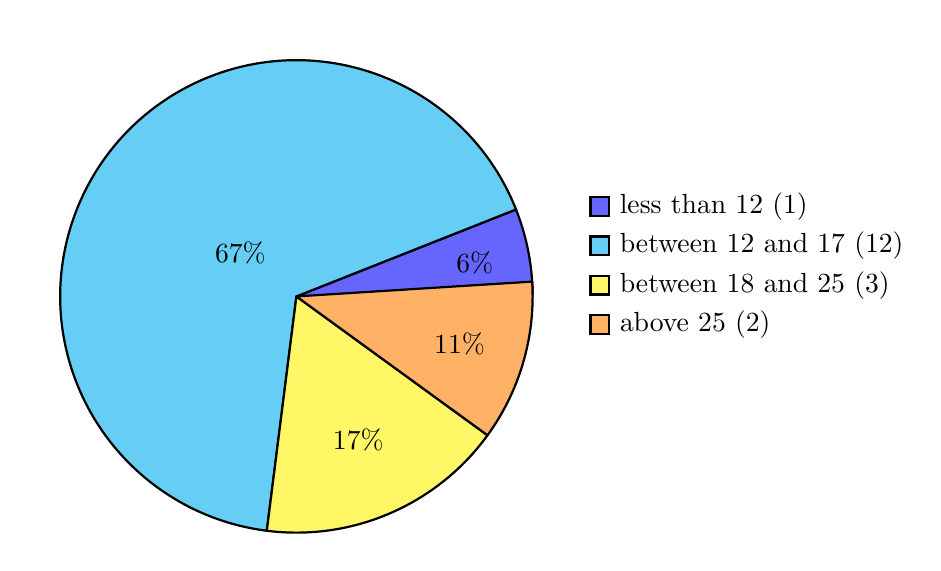
\begin{tikzpicture}
\pie [text=legend]
    {6/less than 12 (1),
    67/between 12 and 17 (12),
    17/between 18 and 25 (3),
    11/above 25 (2)}
\end{tikzpicture}

We can see that the target demographic is teens and above meaning that the game can include some violence. It is important to make the game appropriate to the target demographic as they will be the majority of the player base. 

\parBr

\flushleft{Q2: How much do you play games a week?} \linebreak
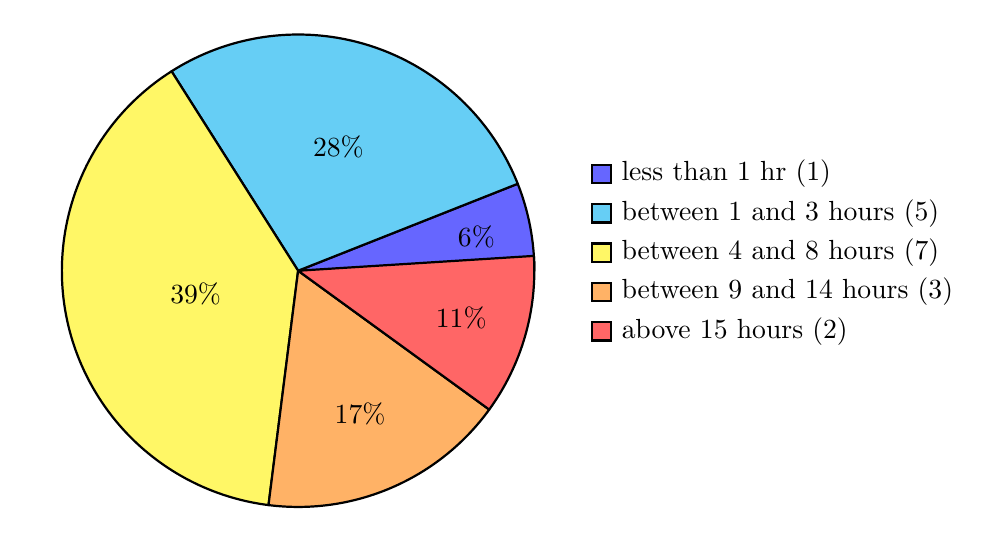
\begin{tikzpicture}
\pie [text=legend]
    {6/less than 1 hr (1),
    28/between 1 and 3 hours (5),
    39/between 4 and 8 hours (7),
    17/between 9 and 14 hours (3),
    11/above 15 hours (2)}
\end{tikzpicture}

It is important to balance the progress made and the time invested as if people only play 1-2hrs a day as shown by the questionnaire, it is important to make the player feel like they made progress in that time so that they are willing to continue playing. This could be implemented by each run being 30-40 mins allowing the user to have a couple runs in a session.

\parBr

\flushleft{Q3: What platform do you play games on?} \linebreak
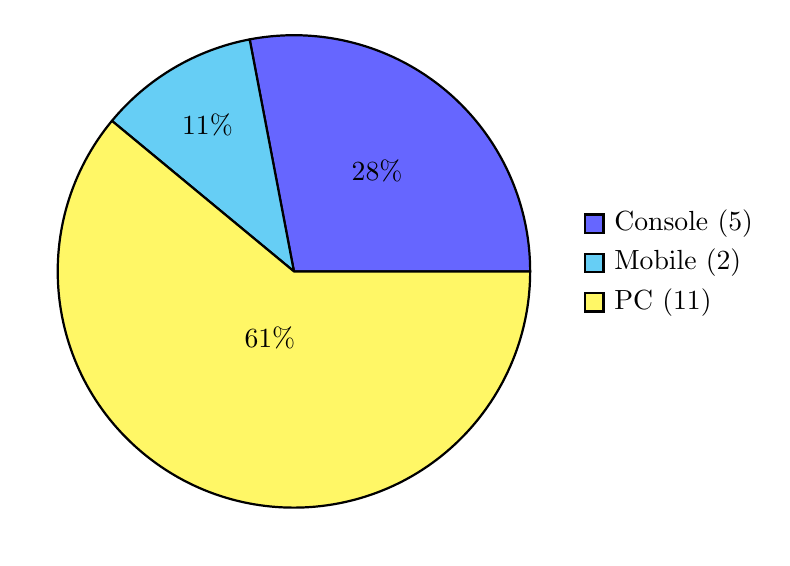
\begin{tikzpicture}
\pie [text=legend]
    {28/Console (5),
    11/Mobile (2),
    61/PC (11)}
\end{tikzpicture}

Most people answered replied that they play on pc meaning that it should be ported to pc first. A significant amount of people also play on console so it would be good to port the game to console if possible. 

\parBr

\flushleft{Q4: what genre of games do you play?} \linebreak
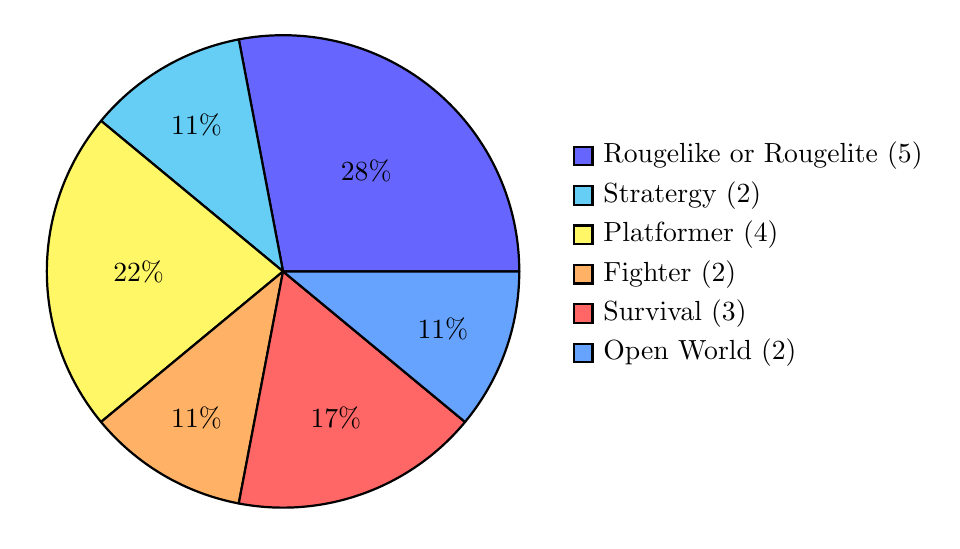
\begin{tikzpicture}
\pie [text=legend]
    {28/Rougelike or Rougelite (5),
    11/Stratergy (2),
    22/Platformer (4),
    11/Fighter (2),
    17/Survival (3),
    11/Open World (2)}
\end{tikzpicture}

\parBr

Most people answered Roguelike/Rougelite and platformer meaning I should focus on these two aspects the most when making my game. Survival will be implemented though planning ahead this might be what routes to take and the risk associated with those routes as well as the risk of combat. As well as management of resources to make sure you survive to the next stage. 

\flushleft{Q5: What mechanics are important to you in a game?} \linebreak
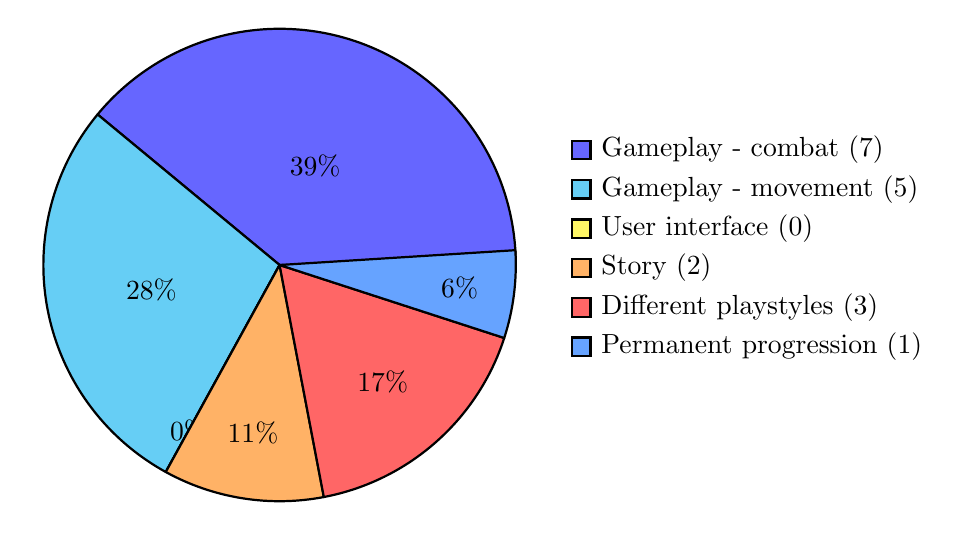
\begin{tikzpicture}
\pie [text=legend]
    {39/Gameplay - combat (7),
	28/Gameplay - movement (5),
	0/User interface (0),
	11/Story (2),
	17/Different playstyles (3),
	6/Permanent progression (1)}
\end{tikzpicture}

\parBr

Combat and movement were the most common option so they should be the most polished systems in the game. Though different playstyles was something I should consider. Permanent progression wasn't a popular choice so a roguelike style would be more suitable 

\flushleft{Q6: how many skills should each character have?} \linebreak
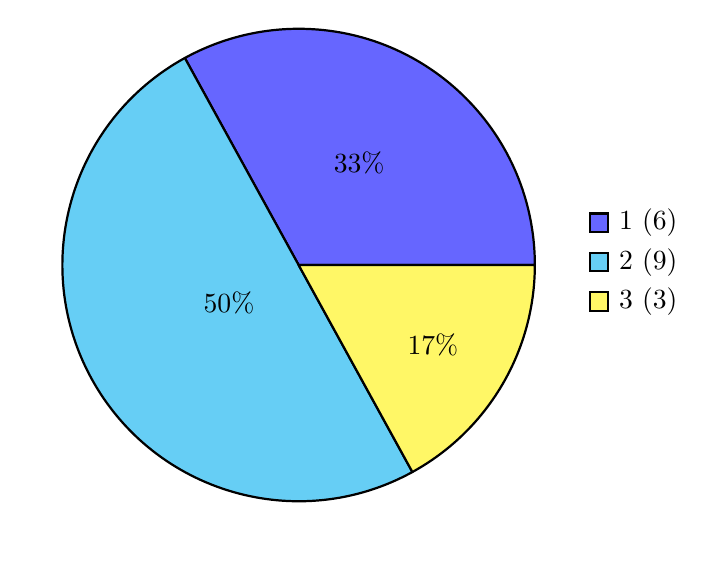
\begin{tikzpicture}
\pie [text=legend]
    {33/1 (6),
    50/2 (9),
    17/3 (3)}
\end{tikzpicture}

\parBr

Most people answered 2 so it would be important to make the skills distinct and unique to allow for different play styles. One ability could be active that the user can activate when needed e.g. throwing grenade and it will have a cool down. The other ability could be a utility skill which can be picked regardless of character and is a limited resource and refreshes once a special item is picked up e.g. throwing knife that does damage, refreshes when more are picked up. There could also be a passive ability that the player doesn't need to do anything to activate it, it will be permanently active in the background (e.g. increased movement speed), this can make every character feel unique. 

\flushleft{Q7: Should each character have their own weapon in their class or be able to?} \linebreak
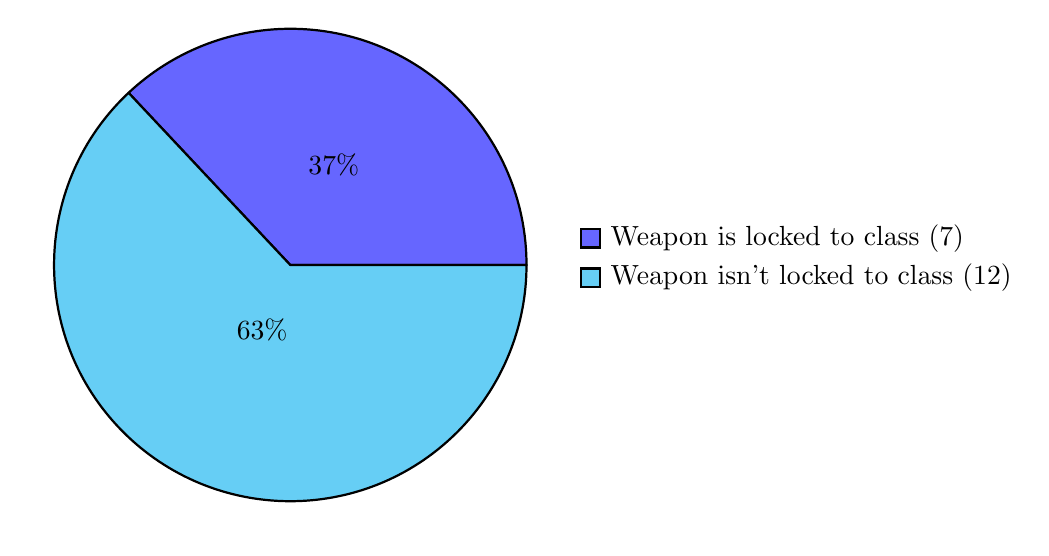
\begin{tikzpicture}
\pie [text=legend]
    {37/Weapon is locked to class (7),
    63/Weapon isn't locked to class (12)}
\end{tikzpicture}

\parBr

The majority wanted to have weapons that are picked up and not locked to a class therefore I will give each character a starting weapon and give them the ability to change this weapon if they wish to, allowing the player to experiment with different weapons that may suit their play style.

\subsection{Analysing Market}
Steam does a hardware analysis on all of it's users every month so I will be able to make a game that will meet the requirements of the majority of players. So all the data in this section is taken from \cite{SHS}

\myparagraph{System OS Analysis}

\begin{figure}[h]
\centering
\includegraphics[width = 0.4\textwidth]{steamOSsurvey}
\caption{\cite{SHS} Steam OS statistics}
\label{steam OS statistics}
\end{figure}

Deciding which systems I will be able to support is going to be an important decision I have to make to make sure that the users can play the game us. Figure \ref{steam OS statistics} shows us that the overwhelming majority of players use windows, this tells me that I should prioritise porting the game to windows as it will make it available to the most amount of players as possible. Mac OS (OS x) only account for a small percentage of players. The difficulties that come with porting my game to Mac simply makes it an inefficient use of time. Linux also accounts for a small percentage of players however porting to Linux is very easy in Godot so it may be something to consider in the future if I have time.

\parBr
\parBr

\myparagraph{Hardware Analysis}
\begin{figure}[h]
\centering
\includegraphics[width = 0.4\textheight]{steamSurvey}
\caption{\cite{SHS} Steam Hardware Statistics}
\label{steam statistics}
\end{figure}

I intend to make a 2D game. These types of games don't tend to be resource intensive. The most important statistics in figure \ref{steam statistics} are system RAM, Intel CPU speeds (More players use Intel CPUs rather than AMD CPUs so this is a valid statistic to use), Physical CPUs, VRAM, Free Hard Disk Space (the ones with a red mark next to them). None of the statistics should be limiting for my project as they would be more important to consider for a 3D game using a fancy rendering system. However my game is 2D so it should be able to run smoothly on most devices.

\subsection{System Requirements}
All the requirements are taken from \cite{spec}, the official Godot 4 documentation.
\paragraph{Minimum Hardware Requirements}
\begin{itemize}
\item Processor: x86\_32 CPU with SSE2 instructions, or any x86\_64 CPU 
\item Graphics Card: Integrated graphics with full Vulkan 1.0 support 
\item Memory: 2GB
\item Storage: Fill out when done
\item Sound Card: yes
\end{itemize}

\paragraph{Input devices:}
\begin{itemize}
\item Keyboard \linebreak 
Allows you to input characters that can be used to control the player
\item Mouse \linebreak
Inputs 2D vector coordinate for mouse position, isn't needed for the 2D vector aspect but it can be used by the player as an optional input method if they desire to use it
\end{itemize}
The input devices allow the user to input signals that the computer to process and adjust accordingly based on the inputs provided.

\paragraph{Output devices:}
\begin{itemize}
\item Display – Outputs image 
\item Speakers – Outputs sound 
\end{itemize}
An example of visualisation since the raw data is presented in a way that the user can comprehend. It also allows them to understand what is happening in the game and feedback on any inputs given.

\paragraph{Minimum Software Requirements}
\begin{itemize}
\item OS: Windows 7+
\end{itemize}


\subsection{Limitations}
Compared to the large studios that produced the games that I researched I have a significant amount of limitations that could slow down the progress of my game development. Such as manpower as studios usually consist of many specialised and trained people. However I am trying to make a game on my own, this means I will need to do everything on my own, from game assets and art to audio design and code. This could be mitigated slightly by the free assets available online which would save me time as I don't have to create them myself.

\parBr

Another limitation is my knowledge and experience in developing games as I only have experience developing one small game for a game jam over the course of a couple days. The project was very limited and used GD script, whereas I would like to use c\# to develop my game. I could overcome  this by following tutorials and doing research to make myself more comfortable with developing my own methodology and ideas.

\parBr

I am also limited by time since there is a deadline I must reach so  I can't continuously develop the game over the course of a couple years. This can be less impactful with good time management and use of abstraction so that I can focus on the main points of the game when developing and spend less time on small features that will go unnoticed for the most part.

\subsection{Essential Features}
One essential feature is the user interface as it allows the user to navigate any menus and displays any important information to the player. The main menu is the first screen that a player would see therefore it is important to give a good  first impression and set the tone of the game and allows the user to start a game and customise their settings. The pause menu is also an important feature of the user interface as it allows the player to pause the game and customise their settings. These things are standard in most games so it would be good to implement it in my game. The HUD (Heads Up Display) is the only user interface that the user sees when they are in game, so it's important to keep it clean and out of the way as it will be overlayed on the users screen at all times. It will also be important to have it display the relevant information, such as the player's health, inventory, and possibly a timer. However not all players will want all of this information on screen at all times so it will be important for the HUD to be customizable to suit a player's needs.

\parBr

Audio is another key feature of games as audio queues can help players fight an enemy, or get feedback since they can hear the sound of their character getting hurt and immediately know that their health has went down without having to look at their health bar. Or when a hit from the player connects with an enemy they know that they damaged the enemy and it also adds to the user experience. This is observed in all the other games I researched, therefore it would be good to include. In game music also sets the tone of the game since if the game changes theme to a combat theme, the player can prepare for combat before the enemies show up.

\parBr

The type of gameplay that I will focus on can be split into two main sections, player combat and player movement. \linebreak
Having a good combat system is important as the player will engage with it very often so it's important for it to feel responsive and fun. This could be done by having a variety of weapons that work well together with the movement system. \linebreak
The movement system will be how the player traverses the level, so having a responsive and fun movement system will be important as the player will always be interacting with it. Allowing for the player to combine movement and combat would create a lot of combinations the player could discover and experiment with.

\parBr

Level generation will also be important as it creates the environment the player will experience the game in. So it needs to work well with the movement system for the levels to be easy to traverse through. Since if the player is unable to reach an important room that could hinder their progress in the game.  

\subsection{Success Criteria}
% split each point into wants and needs
% wants is optional
% needs is manditory
\begin{easylist}
# \large{\textbf{User Interface}}
## \textbf{Main Menu}
### Does it have a new game button? \linebreak
Allows the player to start the game. \smallBr
### Does it have an options button? \linebreak
Allows the player to customise the game to suit them \smallBr
### Does it have a tutorial option? \linebreak
Takes the player to a tutorial level where they can learn the game, important for new players who are playing for the first time. \smallBr
### Does it have a interesting background? \linebreak
Gives a good first impression to the player when they open the game. \smallBr
### Does it have a quit game button? \linebreak
Allows the player to close the game. \smallBr
#### Does it ask you "are you sure"? \linebreak
Makes sure that the played didn't press the button by accident. \smallBr
## \textbf{Pause Menu} 
### Does it pause the game? \linebreak
Allows player to take a break if they need to. \smallBr
### Is there an options button? \linebreak
Allows the player to change setting in game in case they need to. \smallBr
### Is there an exit to main menu button? \linebreak
Allows the player to quit the current run and return to the main menu. \smallBr
#### Does it tell you "The current run will be ended"? \linebreak
Makes sure the player didn't press this button by accident and occidentally quits their run \smallBr
## \textbf{HUD (Heads Up Display)}
### Is there a health bar? \linebreak
Allows player to see their health \smallBr
### Is there a current level box? \linebreak
Allows player to see which stage their on \smallBr
### Is there a timer? \linebreak
Allows player to see how long the run has lasted \smallBr
### Are there small indicators for status effects? \linebreak
Allows player to see if they are affected by and de-buffs/buffs \smallBr
### Is the HUD customisable? \linebreak
Allows player to adjust HUD to their need \smallBr
## \textbf{Inventory}
### Can you drop items?
### Are there item slots?
### Can you rearrange your inventory?
# \large{\textbf{Audio}}
## \textbf{Main Menu}
### Is there some sort of music?
### Do the buttons make a sound?
## \textbf{In Game}
### Is there boss music?
### Does the game have hitting sfx?
### Does the game have a sound for getting hit?
### Does the game have music?
### Does the game have a sound for dying?
# \large{\textbf{Gameplay}}
## \textbf{Level Generation}
### Does it create a level in a reasonable amount of time?
### Are there objects you can interact with that give items?
### Are enemies spawned?
### Is there a safe starting room?
### Is there a boss room at the end?
### Is there variety between levels
## \textbf{Player Combat}
### Does the player die when they have 0 health?
### Can the player melee swing?
### Can the player block?
# \large{\textbf{Visuals}}
\end{easylist}

\section{Designing the Solution}
\subsection{Development Methodology}
There are multiple ways of developing a solution so I've complied a table to summarise all the advantages of disadvantages of each methodology

\pagebreak

\begin{table}[]
\begin{tabular}{|c|l|l|l|l|}
\hline
Methodology & \multicolumn{1}{c|}{Description}                                                                                                                                                         & \multicolumn{1}{c|}{Uses}                                                                                                                          & \multicolumn{1}{c|}{Advantages}                                                                                                                      & \multicolumn{1}{c|}{Disadvantages}                                                                                                                             \\ \hline
Rapid       & \begin{tabular}[c]{@{}l@{}}Iterative methodology where \\ partialy functional prototypes \\ are continually built upon.\end{tabular}                                                     & \begin{tabular}[c]{@{}l@{}}- Small to medium\\    projects\\ - Low budget\\ - Short timeframe\end{tabular}                                         & \begin{tabular}[c]{@{}l@{}}- Flexible to \\   changes\\ - Highly usable \\   product\\ - Focuses on core \\   features\end{tabular}                  & \begin{tabular}[c]{@{}l@{}}- Poorer quality \\   documentation\\ - Fast pace may \\   reduce quality\end{tabular}                                              \\ \hline
Spiral      & \begin{tabular}[c]{@{}l@{}}Goes through four key stages: \\ analysis, risk mitigation, \\ development and evaluation. \\ With each iteration building \\ on the last.\end{tabular}       & \begin{tabular}[c]{@{}l@{}}- Large project\\ - Risk intensive \\   projects\\ - High budget\end{tabular}                                           & \begin{tabular}[c]{@{}l@{}}- Thorough  risk \\   analysis and \\   mitigation\\ - Flexible to \\   changes\\ - Produces \\   prototypes\end{tabular} & \begin{tabular}[c]{@{}l@{}}- Expensive to \\   analyse risks\\ - Lack of focus \\   on efficiency\\ - High costs due \\   to prototypes\end{tabular}           \\ \hline
Agile       & \begin{tabular}[c]{@{}l@{}}Collection of methodlogies \\ which aims to be flexible \\ allowing different sections to \\ be developed in parallel in \\ no particular order.\end{tabular} & \begin{tabular}[c]{@{}l@{}}- Small to medium \\   projects\\ - Unclear initial \\   requirements\end{tabular}                                      & \begin{tabular}[c]{@{}l@{}}- Makes high \\   quality code\\ - Flexible to \\   changes\\ - Regular user \\   input\end{tabular}                      & \begin{tabular}[c]{@{}l@{}}- Poorer quality\\   documentation\\ - Requires consistant \\   interaction between \\   user and programmer\end{tabular}           \\ \hline
Waterfall   & \begin{tabular}[c]{@{}l@{}}Traditianal mode where there \\ is a series of stages which are \\ completed in sequence from \\ start to finish.\end{tabular}                                & \begin{tabular}[c]{@{}l@{}}- Static, low risk \\   project\\ - Require little user \\   input\end{tabular}                                         & \begin{tabular}[c]{@{}l@{}}- Easy to \\   manage\\ - Clearly \\   documented\end{tabular}                                                            & \begin{tabular}[c]{@{}l@{}}- Lack of flexibility\\ - No risk analysis\\ - Limited user \\   involvement\end{tabular}                                           \\ \hline
Extreme     & \begin{tabular}[c]{@{}l@{}}Agile methodology where \\ programmers work alongside \\ and end user to cater to their \\ desires.\end{tabular}                                              & \begin{tabular}[c]{@{}l@{}}- Small to medium \\   projects\\ - Unclear initial \\   requirements\\ - Require excellent \\   usability\end{tabular} & \begin{tabular}[c]{@{}l@{}}- Produces high \\   quality code\\ - Highly usable \\ product\end{tabular}                                               & \begin{tabular}[c]{@{}l@{}}- High cost of two \\   working on project\\ - Teamwork is essential\\ - End user may not be \\   present at all times\end{tabular} \\ \hline
\end{tabular}
\end{table}

To create the code for the game I have designed I have decided to use an agile software development methodology as it's best suited for projects with a small to medium scale with unclear initial requirements, which applies perfectly to my project. It involves creating a prototype based on the user feedback/research and collect user feedback to refine the next iteration and continuously repeat this process until a usable product has been created. This methodology also requires a lot of user feedback which makes the final product very tailored to the stakeholders. It also able to be improved upon continuously until the stakeholders needs are satisfied and all the points on the success criteria are met.

\subsection{Decomposing the problem}
This is one of the computational methods that I am going to use for my game. This is important as it allows me to think of how the game will work at a basic level, instead of considering all the components at once.
\begin{landscape}
\begin{figure}[p]
\centering
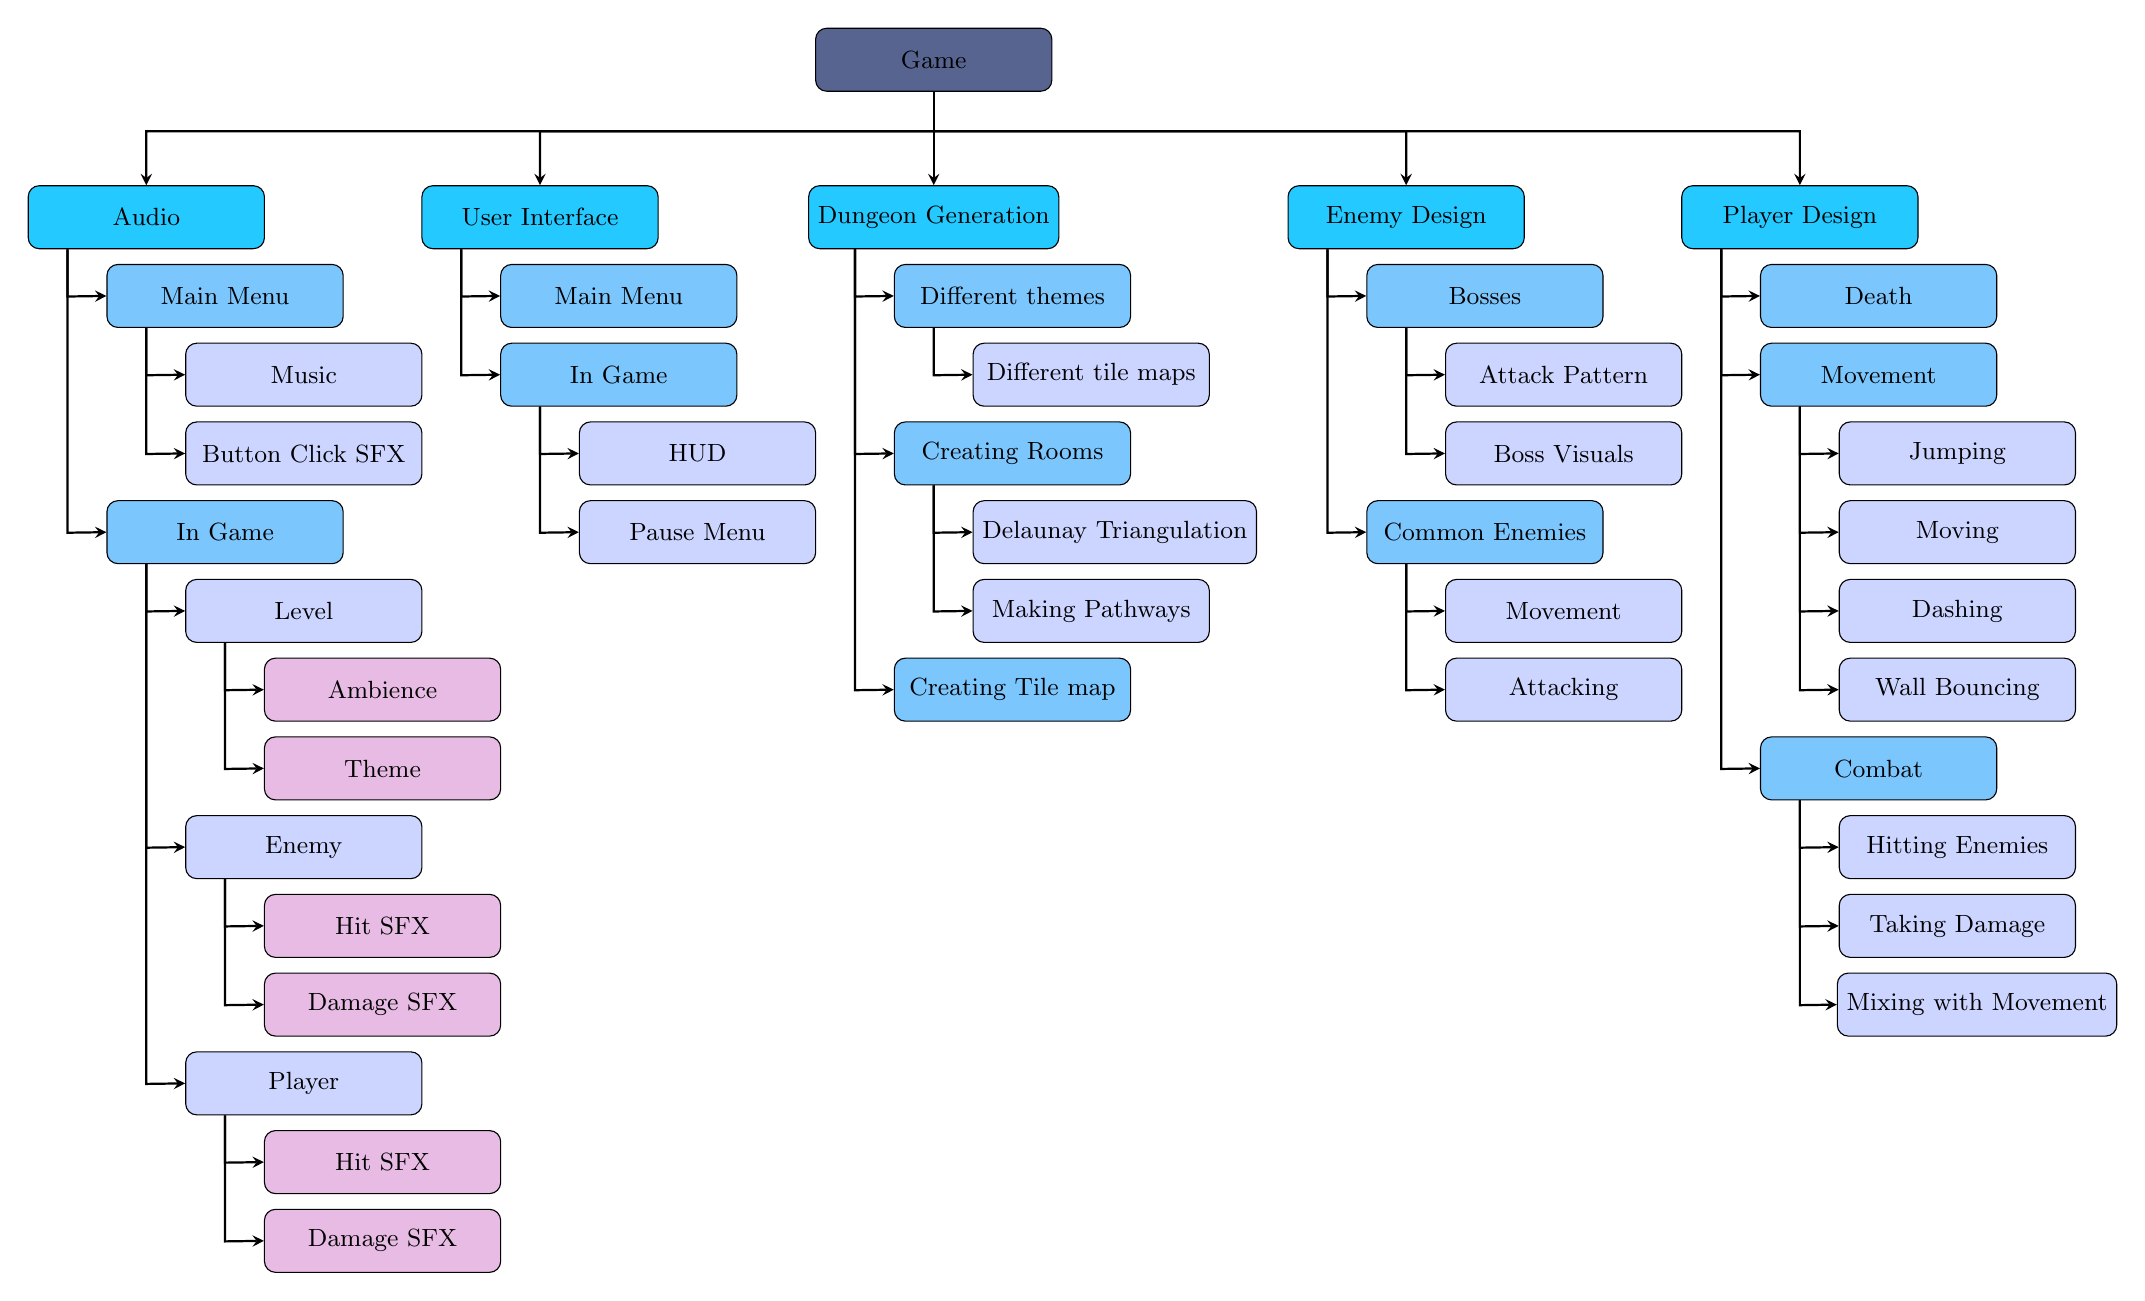
\begin{tikzpicture}[node distance=1cm, every node/.style={font=\small}, align=center]
\node (game) [root] {Game};

%Dungeon Generation
\node (dg) [l1, below of = game,yshift=-1cm] {Dungeon Generation};
\node (layers) [l2, below of=dg, xshift = 1cm] {Different themes};
\node (tilemap) [l3, below of=layers, xshift = 1cm] {Different tile maps};
\node (create) [l2, below of=tilemap, xshift = -1cm] {Creating Rooms};
\node (delaunay) [l3, below of=create, xshift = 1.3cm] {Delaunay Triangulation};
\node (connect) [l3, below of=delaunay,xshift =-0.3cm] {Making Pathways};
\node (ct) [l2, below of=connect, xshift = -1cm] {Creating Tile map};

\draw [arrow] (dg.south)++(-1,0) -- ++(0,-0.6) -- (layers.west);
\draw [arrow] (dg.south)++(-1,0) -- ++(0,-2.6) -- (create.west);
\draw [arrow] (dg.south)++(-1,0) -- ++(0,-5.6) -- (ct.west);
\draw [arrow] (layers.south)++(-1,0) -- ++(0,-0.6) -- (tilemap.west);
\draw [arrow] (create.south)++(-1,0) -- ++(0,-0.6) -- (delaunay.west);
\draw [arrow] (create.south)++(-1,0) -- ++(0,-1.6) -- (connect.west);

%User Interface
\node (ui) [l1, left of= dg, xshift=-4cm] {User Interface};
\node (mm1) [l2, below of= ui, xshift = 1cm] {Main Menu};
\node (ig1) [l2, below of= mm1] {In Game};
\node (hud) [l3, below of= ig1, xshift=1cm] {HUD};
\node (pm) [l3, below of= hud] {Pause Menu};

\draw [arrow] (ui.south)++(-1,0) -- ++(0,-0.6) -- (mm1.west);
\draw [arrow] (ui.south)++(-1,0) -- ++(0,-1.6) -- (ig1.west);
\draw [arrow] (ig1.south)++(-1,0) -- ++(0,-0.6) -- (hud.west);
\draw [arrow] (ig1.south)++(-1,0) -- ++(0,-1.6) -- (pm.west);

%Audio
\node (audio) [l1, left of = ui, xshift=-4cm] {Audio};
\node (mm2) [l2, below of=audio, xshift = 1cm] {Main Menu};
\node (music) [l3, below of=mm2, xshift=1cm] {Music};
\node (bcsfx) [l3, below of=music] {Button Click SFX};
\node (ig2) [l2, below of = bcsfx, xshift=-1cm] {In Game};
\node (level) [l3, below of = ig2, xshift = 1cm] {Level};
\node (ambience) [l4, below of = level, xshift = 1cm] {Ambience};
\node (theme) [l4, below of = ambience] {Theme};
\node (enemy) [l3, below of = theme, xshift = -1cm] {Enemy};
\node (hitsfx1) [l4, below of = enemy, xshift = 1cm] {Hit SFX};
\node (damagesfx1) [l4, below of = hitsfx1] {Damage SFX};
\node (player) [l3, below of = damagesfx1, xshift = -1cm] {Player};
\node (hitsfx2) [l4, below of = player, xshift = 1cm] {Hit SFX};
\node (damagesfx2) [l4, below of = hitsfx2] {Damage SFX};

\draw [arrow] (audio.south)++(-1,0) -- ++(0,-0.6) -- (mm2.west);
\draw [arrow] (audio.south)++(-1,0) -- ++(0,-3.6) -- (ig2.west);
\draw [arrow] (mm2.south)++(-1,0) -- ++(0,-0.6) -- (music.west);
\draw [arrow] (mm2.south)++(-1,0) -- ++(0,-1.6) -- (bcsfx.west);
\draw [arrow] (ig2.south)++(-1,0) -- ++(0,-0.6) -- (level.west);
\draw [arrow] (ig2.south)++(-1,0) -- ++(0,-3.6) -- (enemy.west);
\draw [arrow] (ig2.south)++(-1,0) -- ++(0,-6.6) -- (player.west);
\draw [arrow] (level.south)++(-1,0) -- ++(0,-0.6) -- (ambience.west);
\draw [arrow] (level.south)++(-1,0) -- ++(0,-1.6) -- (theme.west);
\draw [arrow] (enemy.south)++(-1,0) -- ++(0,-0.6) -- (hitsfx1.west);
\draw [arrow] (enemy.south)++(-1,0) -- ++(0,-1.6) -- (damagesfx1.west);
\draw [arrow] (player.south)++(-1,0) -- ++(0,-0.6) -- (hitsfx2.west);
\draw [arrow] (player.south)++(-1,0) -- ++(0,-1.6) -- (damagesfx2.west);

%Enemy Design
\node (ed) [l1, right of = dg, xshift=5cm] {Enemy Design};
\node (boss) [l2, below of=ed, xshift = 1cm] {Bosses};
\node (pattern) [l3, below of=boss, xshift = 1cm] {Attack Pattern};
\node (visual) [l3, below of=pattern] {Boss Visuals};
\node (common) [l2, below of=visual, xshift = -1cm] {Common Enemies};
\node (move1) [l3, below of=common, xshift = 1cm] {Movement};
\node (attack) [l3, below of=move1] {Attacking};

\draw [arrow] (ed.south)++(-1,0) -- ++(0,-0.6) -- (boss.west);
\draw [arrow] (ed.south)++(-1,0) -- ++(0,-3.6) -- (common.west);
\draw [arrow] (boss.south)++(-1,0) -- ++(0,-0.6) -- (pattern.west);
\draw [arrow] (boss.south)++(-1,0) -- ++(0,-1.6) -- (visual.west);
\draw [arrow] (common.south)++(-1,0) -- ++(0,-0.6) -- (move1.west);
\draw [arrow] (common.south)++(-1,0) -- ++(0,-1.6) -- (attack.west);

%Player Desing
\node (pd) [l1, right of = ed, xshift=4cm] {Player Design};
\node (death) [l2, below of=pd, xshift = 1cm] {Death};
\node (move2) [l2, below of=death] {Movement};
\node (jump) [l3, below of=move2, xshift = 1cm] {Jumping};
\node (move3) [l3, below of=jump] {Moving};
\node (dash) [l3, below of=move3] {Dashing};
\node (wall) [l3, below of=dash] {Wall Bouncing};
\node (combat) [l2, below of=wall, xshift = -1cm] {Combat};
\node (hit) [l3, below of=combat, xshift = 1cm] {Hitting Enemies};
\node (dmg) [l3, below of=hit] {Taking Damage};
\node (kill) [l3, below of=dmg,xshift=0.25cm] {Mixing with Movement};

\draw [arrow] (pd.south)++(-1,0) -- ++(0,-0.6) -- (death.west);
\draw [arrow] (pd.south)++(-1,0) -- ++(0,-1.6) -- (move2.west);
\draw [arrow] (pd.south)++(-1,0) -- ++(0,-6.6) -- (combat.west);
\draw [arrow] (move2.south)++(-1,0) -- ++(0,-0.6) -- (jump.west);
\draw [arrow] (move2.south)++(-1,0) -- ++(0,-1.6) -- (move3.west);
\draw [arrow] (move2.south)++(-1,0) -- ++(0,-2.6) -- (dash.west);
\draw [arrow] (move2.south)++(-1,0) -- ++(0,-3.6) -- (wall.west);
\draw [arrow] (combat.south)++(-1,0) -- ++(0,-0.6) -- (hit.west);
\draw [arrow] (combat.south)++(-1,0) -- ++(0,-1.6) -- (dmg.west);
\draw [arrow] (combat.south)++(-1,0) -- ++(0,-2.6) -- (kill.west);

%Root to l1
\draw [arrow] (game.south) -- (dg.north);
\draw [arrow] (game.south)++(0,-0.5) -- ++ (-5,0) -- (ui.north);
\draw [arrow] (game.south)++(0,-0.5) -- ++ (-10,0) -- (audio.north);
\draw [arrow] (game.south)++(0,-0.5) -- ++ (6,0) -- (ed.north);
\draw [arrow] (game.south)++(0,-0.5) -- ++ (11,0) -- (pd.north);
\end{tikzpicture}
\caption{Decomposition Diagram}
\label{decomp}
\end{figure}
\end{landscape}

\subsection{Variable types}   

\myparagraph{Variables}
stores some sort of data in main memory \linebreak \textbf{Data Types}
\begin{itemize}
\item Integer – whole number   
\item Float – real number   
\item Character – single letter/symbol   
\item String – series of characters   
\item Boolean – true or false   
\end{itemize}

CONSTANT – represented as capitalized with underscores
\linebreak
variable – represented as lowercase with underscores 

\subsection{Folder Set up}
% SS of folder setup when complete

\subsection{Dungeon Generation}
The Generation algorithm that I used is a modified version of the algorithm used in {\cite{Gen_Alg}}. The stages I used can be summarised with the key points:
\begin{itemize}
\item{Create rooms}
\item{Spread rooms}
\item{Delete rooms}
\item{Delaunay triangulation}
\item{Remove random amount of edges}
\item{Add spawn and boss room}
\item{Make sure all rooms are accessible}
\item{Turn edges into horizontal and vertical}
\item{Generate corridors}
\item{Turn into tile map}
\item{Spawn player}
\end{itemize}
Some other miscellaneous algorithms used in generation
\begin{itemize}
\item{Turning list of edges to graph}
\item{Turning graph to list of edges}
\end{itemize}

\subsubsection{Create Rooms}
\begin{figure}[h]
\centering
\includegraphics[height = 0.2\textwidth]{room layout}
\includegraphics[height = 0.2\textwidth]{room layout1}
\caption{Room layout example}
\label{Room Layout}
\end{figure}
Begin with generating a defined amount of rooms. Rooms are pre-made layouts that a room as seen in figure \ref{Room Layout}. Originally I generated a cube and gave it a random size, but this would be problematic down the line since when it comes to creating a tile map it would be difficult to generate a room that would be playable \linebreak
This section only needs to generate the rooms.

\begin{figure}[p]
    \centering
    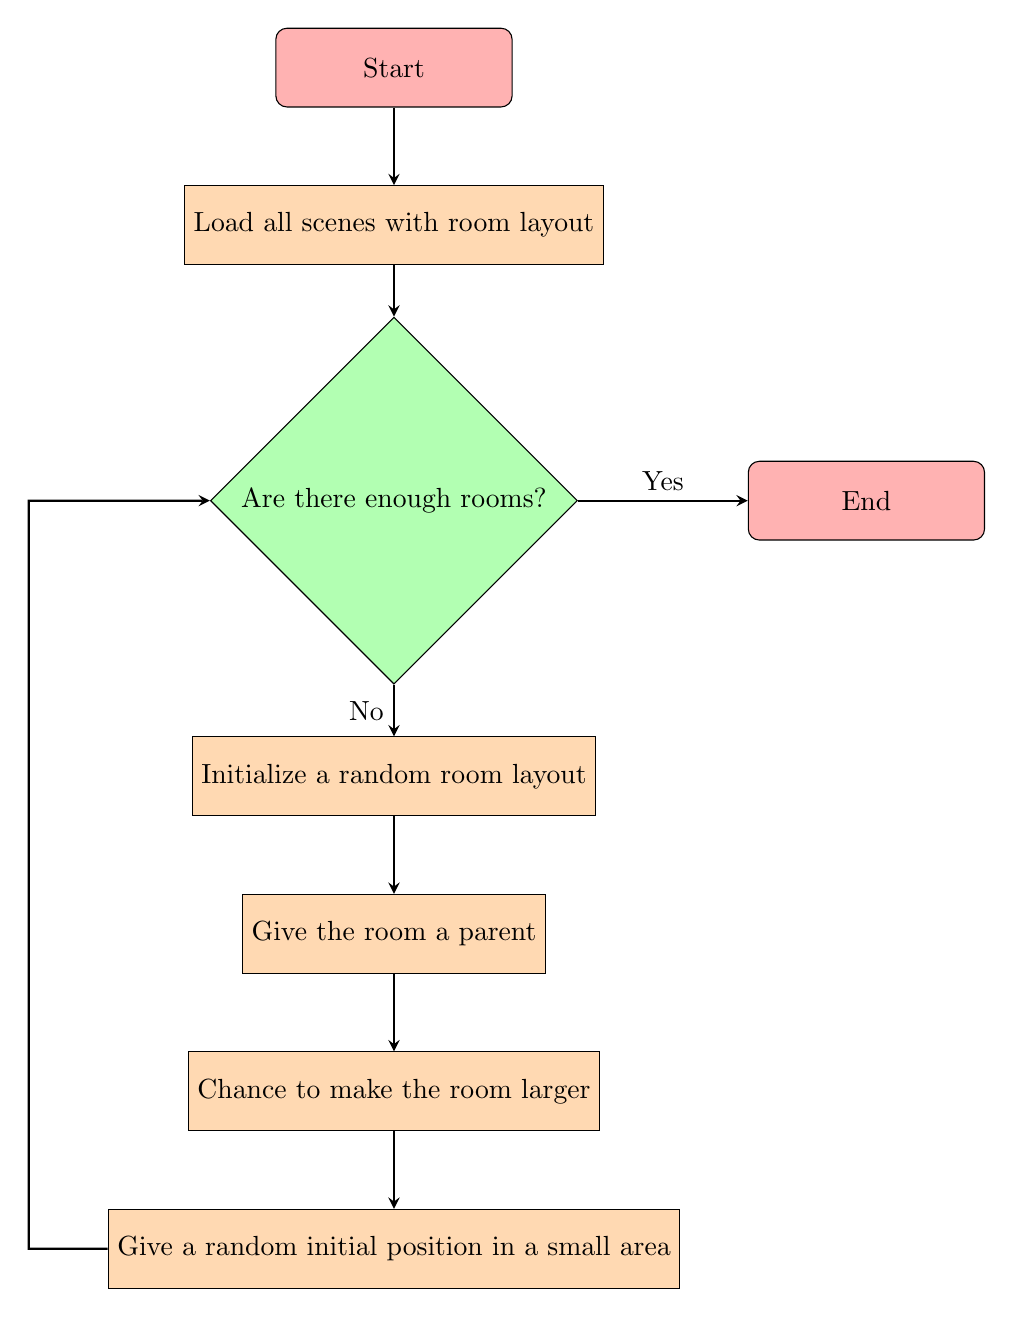
\begin{tikzpicture}[node distance=2cm, align=center]
    \node (start) [startstop] {Start};
    \node (load) [process, below of=start] {Load all scenes with room layout};
    \node (enoughRooms) [decision, below of=load, yshift=-1.5cm] {Are there enough rooms?};
    \node (init) [process, below of=enoughRooms, yshift=-1.5cm] {Initialize a random room layout};
    \node (parent) [process, below of=init] {Give the room a parent};
    \node (chance) [process, below of=parent] {Chance to make the room larger};
    \node (position) [process, below of=chance] {Give a random initial position in a small area};
    \node (stop) [startstop, right of=enoughRooms, xshift=4cm] {End};
    
    \draw [arrow] (start) -- (load);
    \draw [arrow] (load) -- (enoughRooms);
    \draw [arrow] (enoughRooms) -- node[anchor=east] {No} (init);
    \draw [arrow] (position.west) -- ++(-1,0) -- ++(0,9.5)  -- (enoughRooms.west);
    \draw [arrow] (init) -- (parent);
    \draw [arrow] (parent) -- (chance);
    \draw [arrow] (chance) -- (position);
    \draw [arrow] (enoughRooms) -- node[anchor=south] {Yes} (stop);
    
    \end{tikzpicture}
    \caption{Flowchart for generating rooms}
    \label{fig:pseudocode-flowchart}
\end{figure}
\pagebreak

\myparagraph{Pseudocode}
\begin{lstlisting}
load all scenes with room layout
for (int i = 0; i < amountOfRooms; i++)
{
	initialise a random room
	give the room a parent
	chance to make the room larger //for level variation
	give a random initial position in small area
}
\end{lstlisting}

\myparagraph{Variable table} 
\smallBr
\begin{tabular}{l|l|l}
\multicolumn{1}{l|}{Variable Name} & Variable Type                            & \multicolumn{1}{|l}{Description}                             \\ \hline
amountOfRooms                       & Integer                                  & Definse amoubt of room to be generated                       \\
scaleRange                          & Vector2                                  & Defines the min and max scale of a room                      \\
roomVars                            & integer                                  & Tells the program how many room variations exist             \\
randNum                             & Integer                                  & Random integer used for deciding which room type to generate \\
rooms                               & List\textless{}PackedScene\textgreater{} & Contains all possible room variations                        \\
instacne                            & Node                                     & An instance of a room                                       
\end{tabular}

\myparagraph{Identifying test data}
The algorithm will be successful if the following conditions are met:
\begin{itemize}
\item{There is a correct amount of rooms}
\item{There is variation in rooms generated}
\end{itemize}

\subsubsection{Spread rooms}
Once all the rooms are all generated in a confined area they need to be spread out until they are no longer overlapping. To separate the rooms I iterated through each room object and check it for overlapping areas. I found the difference in positions to get the vector of the room relative to the original room being considered, using this I can find the direction that the room should be moved in. This idea was taken from \cite{Dis_Alg}

\begin{figure}[h]
\begin{center}
\includegraphics[width = 0.5\textwidth]{sep_vecs_rects}
\caption{\cite{Dis_Alg} Room Movement Direction}
\end{center}
\label{Room Movement Direction}
\end{figure}

The only major difference in the way that I implemented was that I multiplied the vector by the reciprocal of the magnitude, this would make it so that when there is a colliding room closer to the room being considered it's effect on the displacement of the room is much greater than if it was far from the center of the room

\begin{figure}
\centering
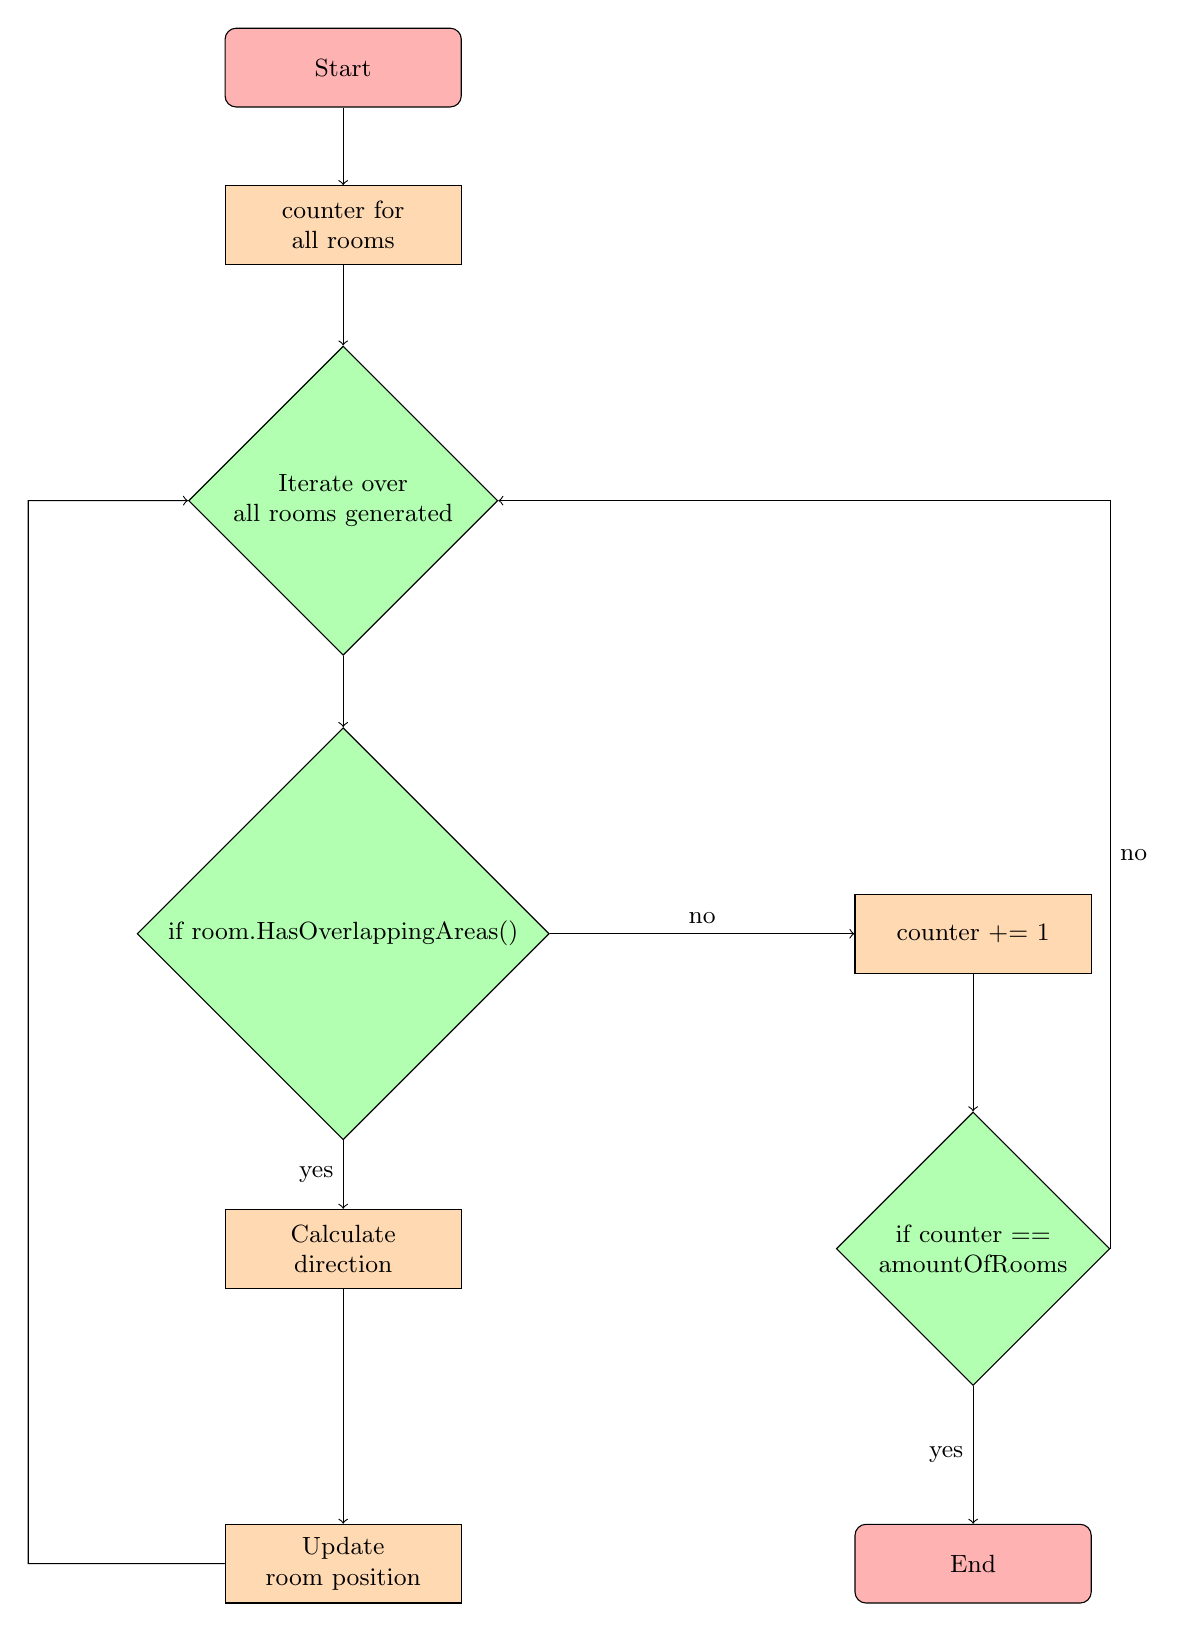
\begin{tikzpicture}[node distance=6cm, every node/.style={font=\small}]

% Nodes
\node (start) [draw, rounded corners, align=center, startstop] {Start};
\node (init) [below of=start, align=center, process, yshift = 4cm] {counter for \\ all rooms};
\node (loop1) [below of=init, align=center, decision, yshift = 2.5cm] {Iterate over \\ all rooms generated};
\node (overlap) [below of=loop1, align=center, decision, yshift = 0.5cm] {if room.HasOverlappingAreas()};
\node (calc) [below of=overlap, align=center, process, yshift = 2cm] {Calculate \\ direction};
\node (update) [below of=calc, align=center, process, yshift = 2cm] {Update \\ room position};
\node (increment) [right of=overlap, xshift=2cm, align=center, process] {counter += 1};
\node (check) [below of=increment, align=center, decision, yshift = 2cm] {if counter == \\ amountOfRooms};
\node (end) [below of=check, align=center, draw, rounded corners, startstop, yshift = 2cm] {End};

% Arrows
\draw [->] (start) -- (init);
\draw [->] (init) -- (loop1);
\draw [->] (loop1) -- (overlap);
\draw [->] (overlap) -- node[anchor=east] {yes} (calc);
\draw [->] (overlap) -- node[anchor=south] {no} (increment);
\draw [->] (calc) -- (update);
\draw [->] (update.west) |- (-4, -19) -- (-4, -5.5)  -- (loop1.west);
\draw [->] (increment) -- (check);
\draw [->] (check) -- node[anchor=east] {yes} (end);
\draw [->] (check.east) -| node[anchor=west, pos=1] {no} ++(0cm,5cm) |- (loop1);

\end{tikzpicture}
\caption{Flowchart for spreading rooms}
\label{fig:fc sep rooms}
\end{figure}
\pagebreak

\textbf{Pseudocode for figure \ref{fig:fc sep rooms}}
\begin{lstlisting}
//this piece of code is called every frame until it develops as solution
checkedRooms = 0
for each room in all_rooms_generated
{
	if room.HasOverlappingAreas()
	{
		direction = Vector2.Zero //sets value to (0,0);
		for each overlappingRoom in room.GetOverlappingAreas()
		{
			displacement = room.Position - overlappingRoom.Position;
			direction += (1/displacement.Length()) * displacement.Normalised;
			//takes reciprocal of displacement and adds it to direction
		}
		//rounds towards nearest int and multiplies by step, which is a variable that scales up with amount of rooms as more rooms will need to spread further which optimizes the algorithm
		direction.X = (float)Math.Round(direction.X) * step;
        direction.Y = (float)Math.Round(direction.Y) * step;
        room.Position += direction
	}
	else
	{
		checkedRooms +=1;
	}
}
if (checkedRooms == amountOfRooms)
{
	//each room has been checked and doesn't have overlapping areas so algorithm finished	
	//move onto next stage of generation
}

\end{lstlisting}

\myparagraph{Variable table}
\smallBr
\begin{tabular}{l|l|l}
Variable Name & Variable Type & Description                                                                                                                         \\ \hline
count         & Integer       & \begin{tabular}[c]{@{}l@{}}Counts the rooms that are separated, if it's equal to room count\\  the section is finished\end{tabular} \\
displacement  & Vector2       & Average displacement vector of all the overlapping rooms                                                                            \\
direction     & Vector2       & Manipulated displacement value to suit the program                                                                                  \\
step          & float         & How far the rooms move each iteration                                                                                              
\end{tabular}

\myparagraph{Identifying test data}
The algorithm will be successful if the following conditions are met:
\begin{itemize}
\item{Rooms don't overlap}
\item{Rooms are still close together}
\item{Spreads in a reasonable amount of time}
\end{itemize}


After this process a pre-defined amount of rooms are deleted so that there are gaps in between the rooms, removing 60\% of the rooms works well. On top of this the position of each room is multiplied by 2 to spread the rooms further

\subsubsection{Delete Rooms}
The rooms being too close together means that all the corridors will be short and it will be uneventful. Therefore deleting a certain percentage of rooms will make the level more interesting for the player as they will be spread unevenly. To spread the rooms apart further without having to generate more rooms and deleter them we can also multiply the position of each room to spread them apart further. This will make the algorithm more efficient because the program doesn't need to generate more rooms to get the same effect.
\linebreak \linebreak

\begin{figure}[h]
  \centering
  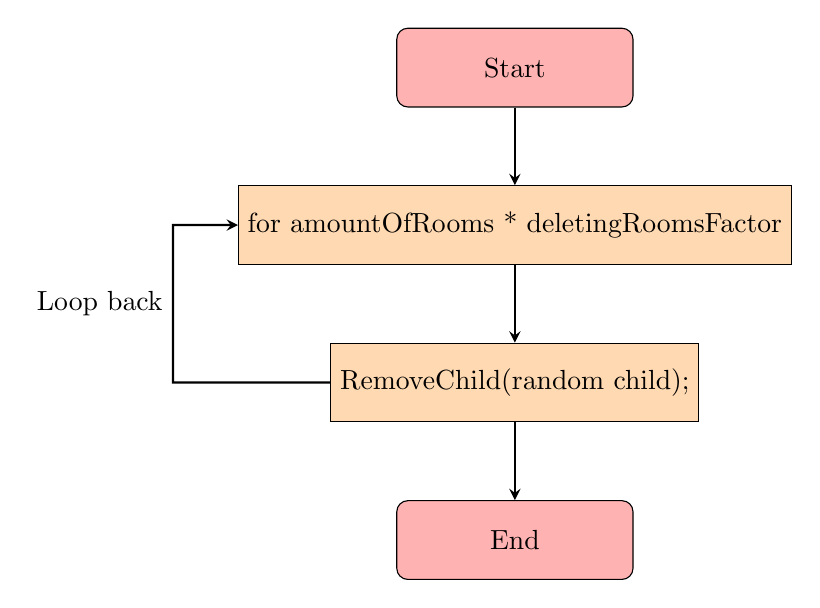
\begin{tikzpicture}[node distance=2cm, align=center]
    \node (start) [startstop] {Start};
    \node (forloop) [process, below of=start] {for amountOfRooms * deletingRoomsFactor};
    \node (removechild) [process, below of=forloop] {RemoveChild(random child);};
    \node (end) [startstop, below of=removechild] {End};
    
    \draw [arrow] (start) -- (forloop);
    \draw [arrow] (forloop) -- (removechild);
    \draw [arrow] (removechild) -- (end);
    \draw [arrow] (removechild.west) -- ++(-2,0) node[anchor=east, yshift=1cm] {Loop back} -- ++(0,2) -- (forloop.west);
  \end{tikzpicture}
  \caption{Flowchart for deleting rooms}
  \label{deleting flowchart}
\end{figure}

\textbf{Pseudocode for figure \ref{deleting flowchart}}
\begin{lstlisting}
for (int)(amountOfRooms * deletingRoomsFactor);
{
    RemoveChild(random child);
}
\end{lstlisting}

\myparagraph{Variable table}
\smallBr
\begin{tabular}{l|l|l}
Variable Name       & Variable Type & Description                                                         \\ \hline
deletingRoomsFactor & float         & Needs to be between 0-1 (if its 0.8 it will delete 80\% of rooms)
\end{tabular}

\myparagraph{Identifying test data}
The algorithm will be successful if the following conditions are met:
\begin{itemize}
\item{Rooms are spread apart without being on top of each other}
\item{Distance between rooms varies}
\end{itemize}

\subsubsection{Delaunay Triangulation}
The algorithm used in this section was taken from \cite{BW_alg}(Bowyer–Watson algorithm). For the algorithm to function I needed a data structure for points, which link the Area2D, position and a list of points which the point is connected to. Edges are an array of two points which represents a connection between two points. Triangles are an array of three edges and hence three points, from these a circumcircle can be drawn, which is important for the Bowyer-Watson algorithm, this is represented as a vector2 storing the circumcentre and a float for the radius.
\linebreak
\begin{figure}
\begin{center}
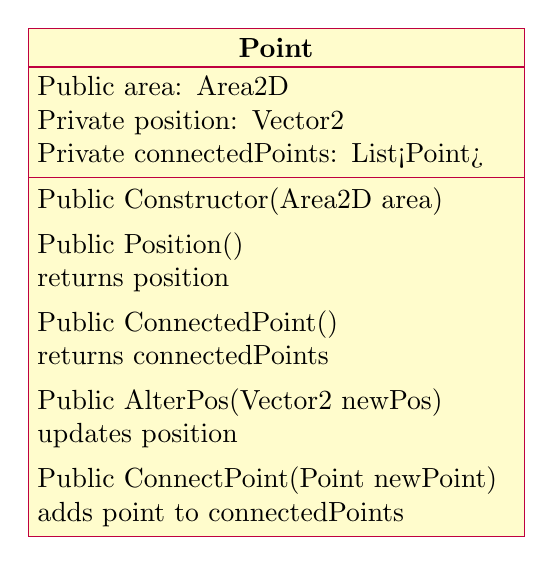
\begin{tikzpicture}
\begin{class}[text width = 0.5\textwidth]{Point}{0 ,0}
\attribute{Public area: Area2D}
\attribute{Private position: Vector2}
\attribute{Private connectedPoints: List<Point>} 
\operation{Public Constructor(Area2D area) \smallBr}
\operation{Public Position() \linebreak returns position \smallBr}
\operation{Public ConnectedPoint() \linebreak returns connectedPoints \smallBr}
\operation{Public AlterPos(Vector2 newPos) \linebreak updates position \smallBr}
\operation{Public ConnectPoint(Point newPoint) \linebreak adds point to connectedPoints}
\end{class}
\end{tikzpicture}

\parBr

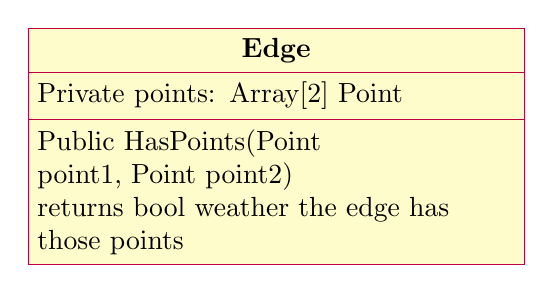
\begin{tikzpicture}
\begin{class}[text width = 0.5\textwidth]{Edge}{0 ,0}
\attribute{Private points: Array[2] Point}
\operation{Public HasPoints(Point point1, Point point2) \linebreak returns bool weather the edge has those points}
\end{class}
\end{tikzpicture}

\parBr

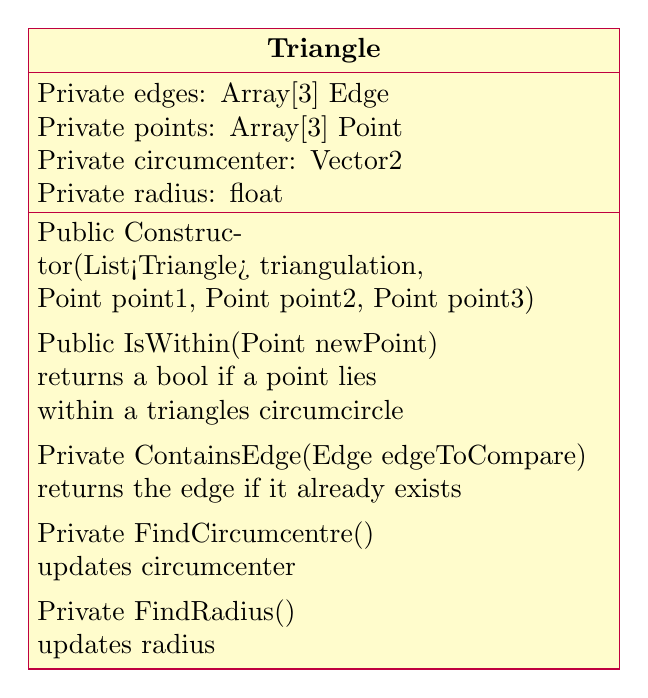
\begin{tikzpicture}
\begin{class}[text width =0.6\textwidth]{Triangle}{0 ,0}
\attribute{Private edges: Array[3] Edge}
\attribute{Private points: Array[3] Point}
\attribute{Private circumcenter: Vector2}
\attribute{Private radius: float}
\operation{Public Constructor(List<Triangle> triangulation, \linebreak Point point1, Point point2, Point point3) \smallBr}
\operation{Public IsWithin(Point newPoint) \linebreak returns a bool if a point lies within a triangles circumcircle \smallBr}
\operation{Private ContainsEdge(Edge edgeToCompare) \linebreak returns the edge if it already exists \smallBr}
\operation{Private FindCircumcentre() \linebreak updates circumcenter \smallBr}
\operation{Private FindRadius()\linebreak updates radius}
\end{class}
\end{tikzpicture}
\end{center}
\caption{Bowyer-Watson Classes}
\label{bw class}
\end{figure}


\begin{figure}
\centering
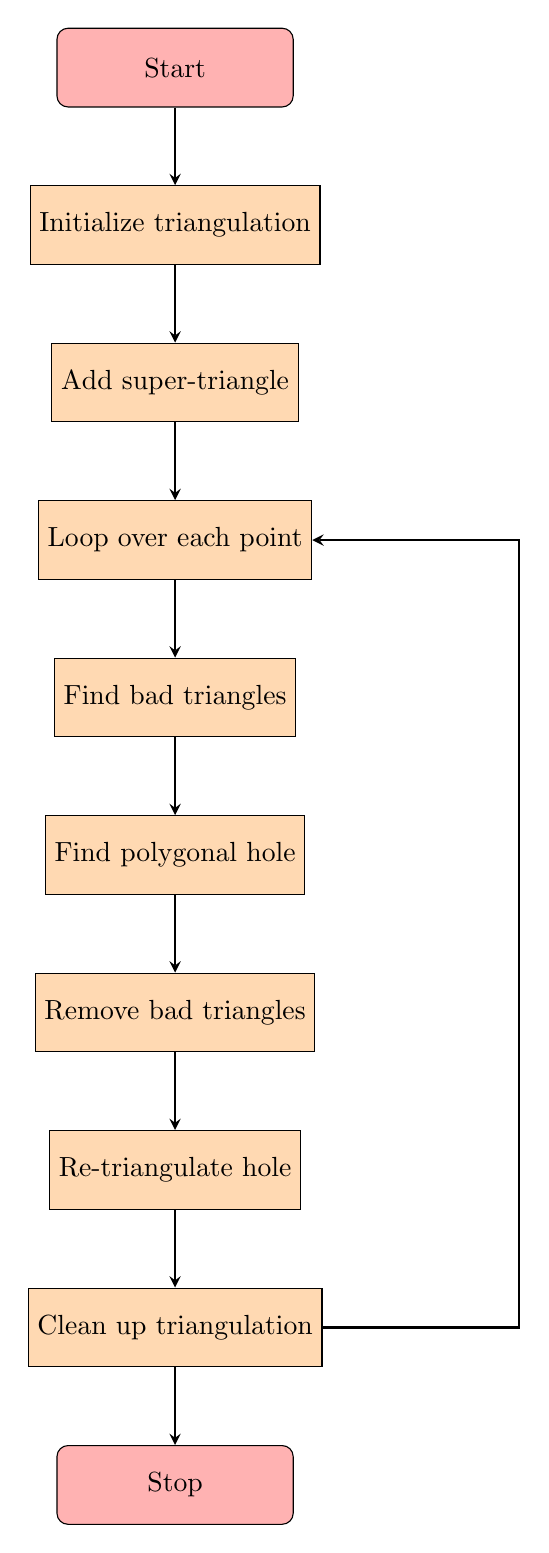
\begin{tikzpicture}[node distance=2cm, auto]

% Nodes
\node (start) [startstop] {Start};
\node (init) [process, below of=start] {Initialize triangulation};
\node (addSuperTriangle) [process, below of=init] {Add super-triangle};
\node (loopStart) [process, below of=addSuperTriangle] {Loop over each point};
\node (findBadTriangles) [process, below of=loopStart] {Find bad triangles};
\node (findPolygon) [process, below of=findBadTriangles] {Find polygonal hole};
\node (removeBadTriangles) [process, below of=findPolygon] {Remove bad triangles};
\node (retriangulate) [process, below of=removeBadTriangles] {Re-triangulate hole};
\node (cleanUp) [process, below of=retriangulate] {Clean up triangulation};
\node (stop) [startstop, below of=cleanUp] {Stop};

% Arrows
\draw [arrow] (start) -- (init);
\draw [arrow] (init) -- (addSuperTriangle);
\draw [arrow] (addSuperTriangle) -- (loopStart);
\draw [arrow] (loopStart) -- (findBadTriangles);
\draw [arrow] (findBadTriangles) -- (findPolygon);
\draw [arrow] (findPolygon) -- (removeBadTriangles);
\draw [arrow] (removeBadTriangles) -- (retriangulate);
\draw [arrow] (retriangulate) -- (cleanUp);
\draw [arrow] (cleanUp) -- (stop);

% Loop back arrow
\draw [arrow] (cleanUp.east) -- ++(2.5,0) |- (loopStart.east);

\end{tikzpicture}
\caption{Bowyer-Watson Algorithm Flowchart}
\label{fig:bowyer_watson_flowchart}
\end{figure}
\pagebreak

\textbf{Pseudocode for figure \ref{fig:bowyer_watson_flowchart}} \linebreak
\textit{The pseudocode was taken from} \cite{BW_alg}
\begin{lstlisting}
function BowyerWatson (pointList)
    // pointList is a list of points defining the points to be triangulated
    triangulation := empty list of triangles
    add super-triangle to triangulation // must be large enough to completely contain all the points in pointList
    for each point in pointList do // add all the points one at a time to the triangulation
        badTriangles := empty list of triangles
        for each triangle in triangulation do // first find all the triangles that are no longer valid due to the insertion
            if point is inside circumcircle of triangle
                add triangle to badTriangles
        polygon := list of edges
        for each triangle in badTriangles do // find the boundary of the polygonal hole
            for each edge in triangle do
                if edge is not shared by any other triangles in badTriangles
                    add edge to polygon
        for each triangle in badTriangles do // remove them from the data structure
            remove triangle from triangulation
        for each edge in polygon do // re-triangulate the polygonal hole
            newTri := form a triangle from edge to the new point
            add newTri to triangulation
    for each triangle in triangulation // done inserting points, now clean up
        if triangle contains a vertex from original super-triangle
            remove triangle from triangulation
    return triangulation
\end{lstlisting}

\myparagraph{Variable table}
\smallBr
\begin{tabular}{l|l|l}
Variable Name   & Variable Type                         & Description                                 \\ \hline
triangulation   & List\textless{}Triangle\textgreater{} & List of the triangulated mesh               \\
badTriangles    & List\textless{}Triangle\textgreater{} & List of triangles to discard                \\
polygon         & List\textless{}Edge\textgreater{}     & All edges in end result                     \\
polygonEdgeList & List\textless{}Edge\textgreater{}     & List of edges to retriangulate to new point \\
superTriPoint1  & Point                                 & Point of triangle surrounding all points    \\
superTriPoint2  & Point                                 & Point of triangle surrounding all points    \\
superTriPoint3  & Point                                 & Point of triangle surrounding all points    \\
point           & Point                                 & Point being added to the triangulation      \\
allPoints       & List\textless{}Point\textgreater{}    & List of all points to be triangulated      
\end{tabular}

\myparagraph{Identifying test data}
The algorithm will be successful if the following conditions are met:
\begin{itemize}
\item{Triangulated in the most efficient way possible}
\item{Every room is included in the triangulation}
\item{Computes in a reasonable amount of time}
\end{itemize}

\parBr
The pseudo code states that there needs to be triangles, edges and points. These structures can be achieved with object oriented programming as I can make a class with all the relevant attributes and methods for each data structure mentioned.

\subsubsection{Remove random amount of edges}
Figure \ref{bwa result} shows the result of the algorithm, however this many corridors would be overwhelming for players and would result in each room having 4-5 corridors leading out of it, which would could overwhelm the player. Other rouge-like games usually contain 2-3 corridors leading out of it, this would mean I needed to delete some of the edges but still make sure all the rooms are accessible.

\parBr

Currently the mesh is stored as a list of edges. So to remove a certain amount I can make a copy of the list and then remove a random amount of edges. However C\# passes the list by reference so any alterations on the copy of the list will also alter the original. Therefore I made a new empty list and added a random amount of edges from the original list.

\begin{figure}[p]
    \centering
    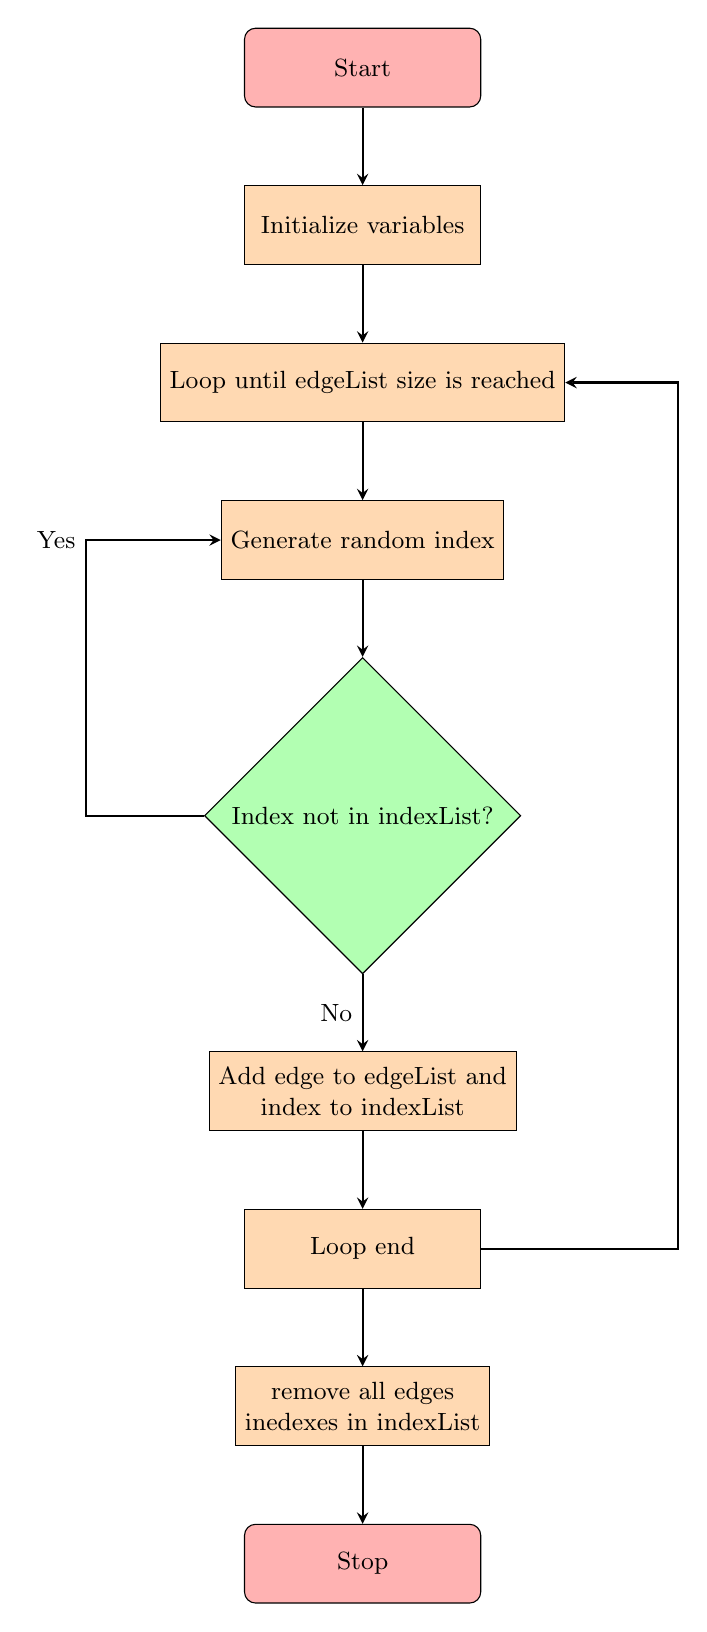
\begin{tikzpicture}[node distance=2cm, every node/.style={font=\small}, align=center]
    % Nodes
    \node (start) [startstop] {Start};
    \node (init) [process, below of=start] {Initialize variables};
    \node (loopStart) [process, below of=init] {Loop until edgeList size is reached};
    \node (generateRandomIndex) [process, below of=loopStart] {Generate random index};
    \node (checkDuplicate) [decision, below of=generateRandomIndex, yshift=-1.5cm] {Index not in indexList?};
    \node (addEdgeToList) [process, below of=checkDuplicate, yshift=-1.5cm] {Add edge to edgeList and \\ index to indexList};
    \node (loopEnd) [process, below of=addEdgeToList] {Loop end};
    \node (del) [process, below of=loopEnd] {remove all edges \\ inedexes in indexList};
    \node (stop) [startstop, below of=del] {Stop};
    
    % Arrows
    \draw [arrow] (start) -- (init);
    \draw [arrow] (init) -- (loopStart);
    \draw [arrow] (loopStart) -- (generateRandomIndex);
    \draw [arrow] (generateRandomIndex) -- (checkDuplicate);
    \draw [arrow] (checkDuplicate) -- node[anchor=east] {No} (addEdgeToList);
    \draw [arrow] (checkDuplicate.west) -- ++(-1.5,0) |- node[anchor=east] {Yes} (generateRandomIndex.west);
    \draw [arrow] (addEdgeToList) -- (loopEnd);
    \draw [arrow] (loopEnd.east) -- ++(2.5,0) |- (loopStart.east);
    \draw [arrow] (loopEnd) -- (del);
    \draw [arrow] (del) -- (stop);

    \end{tikzpicture}
    \caption{Flowchart for Edge Deletion Algorithm}
    \label{fig:edge-deletion}
\end{figure}

\pagebreak

\textbf{Pseudocode for figure \ref{fig:edge-deletion}}
\begin{lstlisting}
float edgeDeletingFactor; //number between 0-1 representing how much edges to keep
List<Edge> polygon; //List of edges from triangulation stage
List<Edge> edgeList = new List<Edge>();
List<int> indexList = new List<int>();
int newIndex;
while (edgeList.Count() < (int)(polygon.Count()* edgeDeletingFactor))
{
	newIndex = RandomIntBetween(0,polygon.Count())
	//this part ensures there is no duplicates in edgeList
	if (!indexList.Contains(newIndex))
	{
		edgeList.Add(polygon[newIndex]);
		indexList.Add(newIndex);
	}
}
\end{lstlisting}

\myparagraph{Variable table}
\smallBr
\begin{tabular}{l|l|l}
Variable Name      & Variable Type                    & Description                                                     \\ \hline
edgeDeletingFactor & float                            & Needs to be between 0-1 (if its 0.8 it will keep 80\% of edges) \\
indexList          & List\textless{}int\textgreater{} & List of indexes to remove from edge list                        \\
newIndex           & int                              & New index to be checked if it can be deleted                   
\end{tabular}

\myparagraph{Identifying test data}
The algorithm will be successful if the following conditions are met:
\begin{itemize}
\item{Random amount of edges is deleted}
\end{itemize}

\parBr

However this creates a problem as now some of the rooms are inaccessible because they have no edges connecting to them or are in another inaccessible section. This is solved in the next section.

\subsubsection{Generate spawn and boss room}
Before connecting each room to each other we need to have the player a starting position and a goal, this will be done by creating a spawn room where the player starts, this room will always be at the top of the map and force the player to go down. The boss room will always be generated at the bottom of the map since it's the goal for the player to reach. Therefore the player can always go down if they are stuck or unsure as to where to go. 

\begin{figure}[p]
    \centering
    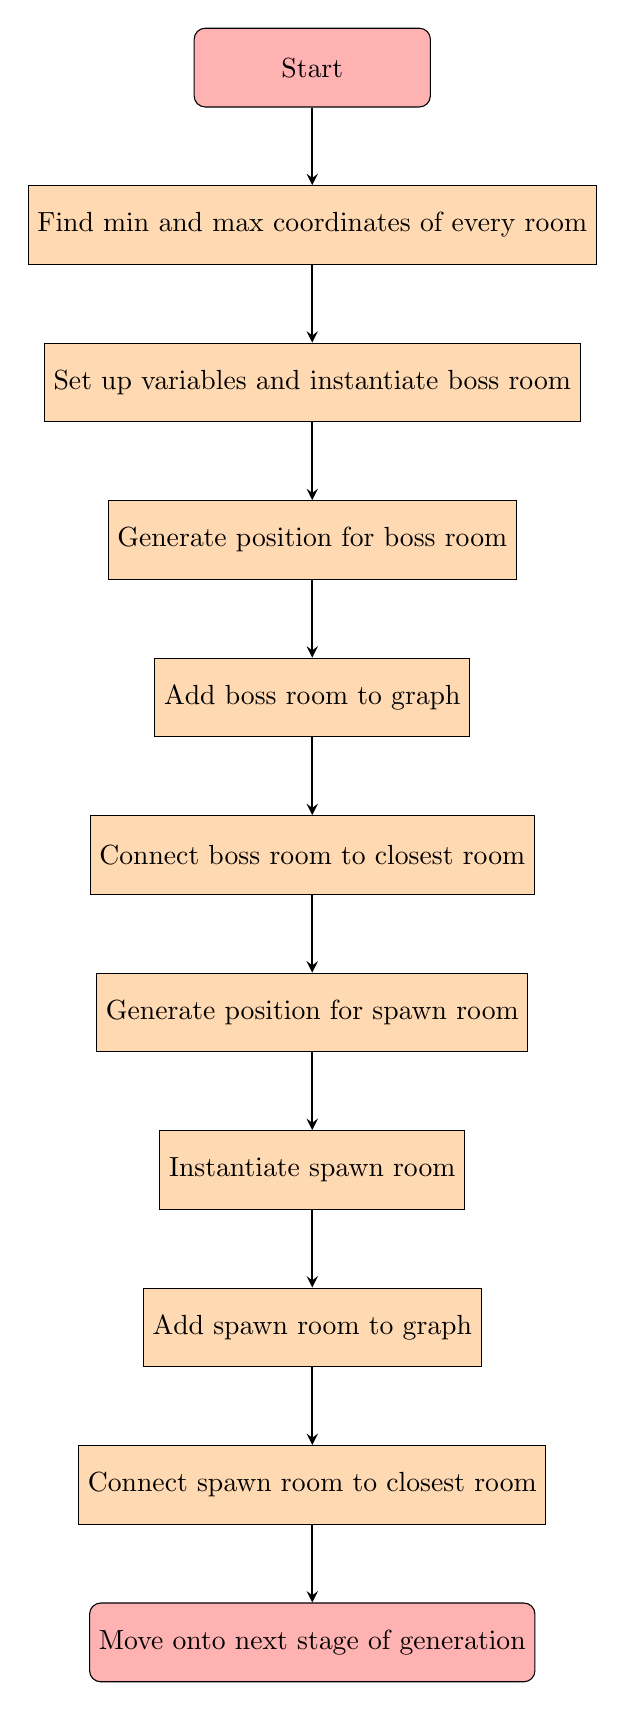
\begin{tikzpicture}[node distance=2cm]
    \node (start) [startstop] {Start};
    \node (minmax) [process, below of=start] {Find min and max coordinates of every room};
    \node (setup) [process, below of=minmax] {Set up variables and instantiate boss room};
    \node (genposboss) [process, below of=setup] {Generate position for boss room};
    \node (addboss) [process, below of=genposboss] {Add boss room to graph};
    \node (connectboss) [process, below of=addboss] {Connect boss room to closest room};
    \node (genspawn) [process, below of=connectboss] {Generate position for spawn room};
    \node (spawnroom) [process, below of=genspawn] {Instantiate spawn room};
    \node (addspawn) [process, below of=spawnroom] {Add spawn room to graph};
    \node (connectspawn) [process, below of=addspawn] {Connect spawn room to closest room};
    \node (nextstage) [startstop, below of=connectspawn] {Move onto next stage of generation};
    
    \draw [arrow] (start) -- (minmax);
    \draw [arrow] (minmax) -- (setup);
    \draw [arrow] (setup) -- (genposboss);
    \draw [arrow] (genposboss) -- (addboss);
    \draw [arrow] (addboss) -- (connectboss);
    \draw [arrow] (connectboss) -- (genspawn);
    \draw [arrow] (genspawn) -- (spawnroom);
    \draw [arrow] (spawnroom) -- (addspawn);
    \draw [arrow] (addspawn) -- (connectspawn);
    \draw [arrow] (connectspawn) -- (nextstage);
    
    \end{tikzpicture}
    \caption{Flowchart for Generating spawn and boss rooms}
    \label{gen spanwboss}
\end{figure}

\pagebreak

\textbf{Pseudocode for figure \ref{gen spanwboss}}
\begin{lstlisting}
//polygon is the list of edges where we have to connect new room, its taken from the previous section
Find min and max coordinate of every room
//set up variables needed
List<Point> graph = MakeGraph(polygon);
Point closestPoint;
instantiate bossRoom
AddChild(bossRoom);
//label it so that it can be identified
bossRoom.Name = "rmB";
//genereate position between min and max X coord but bias for center
//Make Y coord certain amount below other rooms.
bossRoom.Position.X = minCoord.X + rng.RandfRange(0.2f, 0.8f) * (maxCoord.X - minCoord.X)
//(0,1) is down in godot so we take maxcoord for y position to place it at the bottom
bossRoom.Position.Y = maxCoord.Y + roomDist);
//Make boss room into a point to add it to graph
Point bossPoint = new Point(bossRoom);
graph.Add(bossPoint);
foreach (point in graph)
{
    if (point is closer to bossRoom then current closest known point)
    {
        closestPoint = point;
    }
}
//connect boss to closest room
bossPoint.ConnectPoint(closestPoint);
closestPoint.ConnectPoint(bossPoint);
//Do same thing for spawn room
instantiate spawnRoom
AddChild(spawnRoom);
//lable room to make it easy to identify
spawnRoom.Name = "rmS";
//genereate position between min and max X coord but bias center more
//Make Y coord certain amount above other rooms.
bossRoom.Position.X = minCoord.X + rng.RandfRange(0.2f, 0.8f) * (maxCoord.X - minCoord.X)
//(0,-1) is up in godot so we take mincoord for y position to place it at the top
bossRoom.Position.Y = minCoord.Y - roomDist);
//Make spawn room into a point to add it to graph
Point spawnPoint = new Point(spawnRoom);
graph.Add(spawnPoint);
//reset value of closest point
closestPoint = null;
foreach (point in graph)
{
    if (point is closer to spawnRoom than currently closest known point)
    {
        closestPoint = room;
    }
}
//connect spawn to closest room
spawnPoint.ConnectPoint(closestPoint);
closestPoint.ConnectPoint(spawnPoint);

Move onto next stage of generation
\end{lstlisting}

\myparagraph{Variable table}
\smallBr
\begin{tabular}{l|l|l}
Variable Name   & Variable Type                      & Description                                                     \\ \hline
closestPoint    & Point                              & Closest known point to room that is being generated             \\
graph           & List\textless{}Point\textgreater{} & List of all the rooms that have been generated                  \\
currentLength   & float                              & distance between closest known point and room being generated   \\
bossRoom        & Node                               & The actual boss room                                            \\
bossPoint       & Point                              & bossRoom turned to a point                                      \\
spawnRoom       & Node                               & The actual spawn room                                           \\
spawnPoint      & Point                              & spawnRoom turned into a point                                   \\
polygonEdgeList & List\textless{}Edge\textgreater{}  & List of all the edges that compose the current state of the map
\end{tabular}

\myparagraph{Identifying test data}
The algorithm will be successful if the following conditions are met:
\begin{itemize}
\item{Spawn room and boss room are generated}
\item{Spawn is generated above all other rooms}
\item{Boss room is generated below all other rooms}
\item{Both rooms are generated relatively close to the center}
\end{itemize}

\subsubsection{Make sure all rooms are accessible}
This section can be decomposed into smaller problems. That being detecting a single section and detecting all sections, then making sure they are connected. First comes detecting sections, this is accomplished more easily when the the graph is represented with list of points along with each point having a list of points it's connected to. Currently the graph is represented as a list of edges. This can be done with a simple algorithm explored further in the "Turning list of edge to graph" section. The detecting sections part is an example of depth first graph traversal since algorithm identifies leaf nodes first.

\begin{figure}[p]
  \centering
  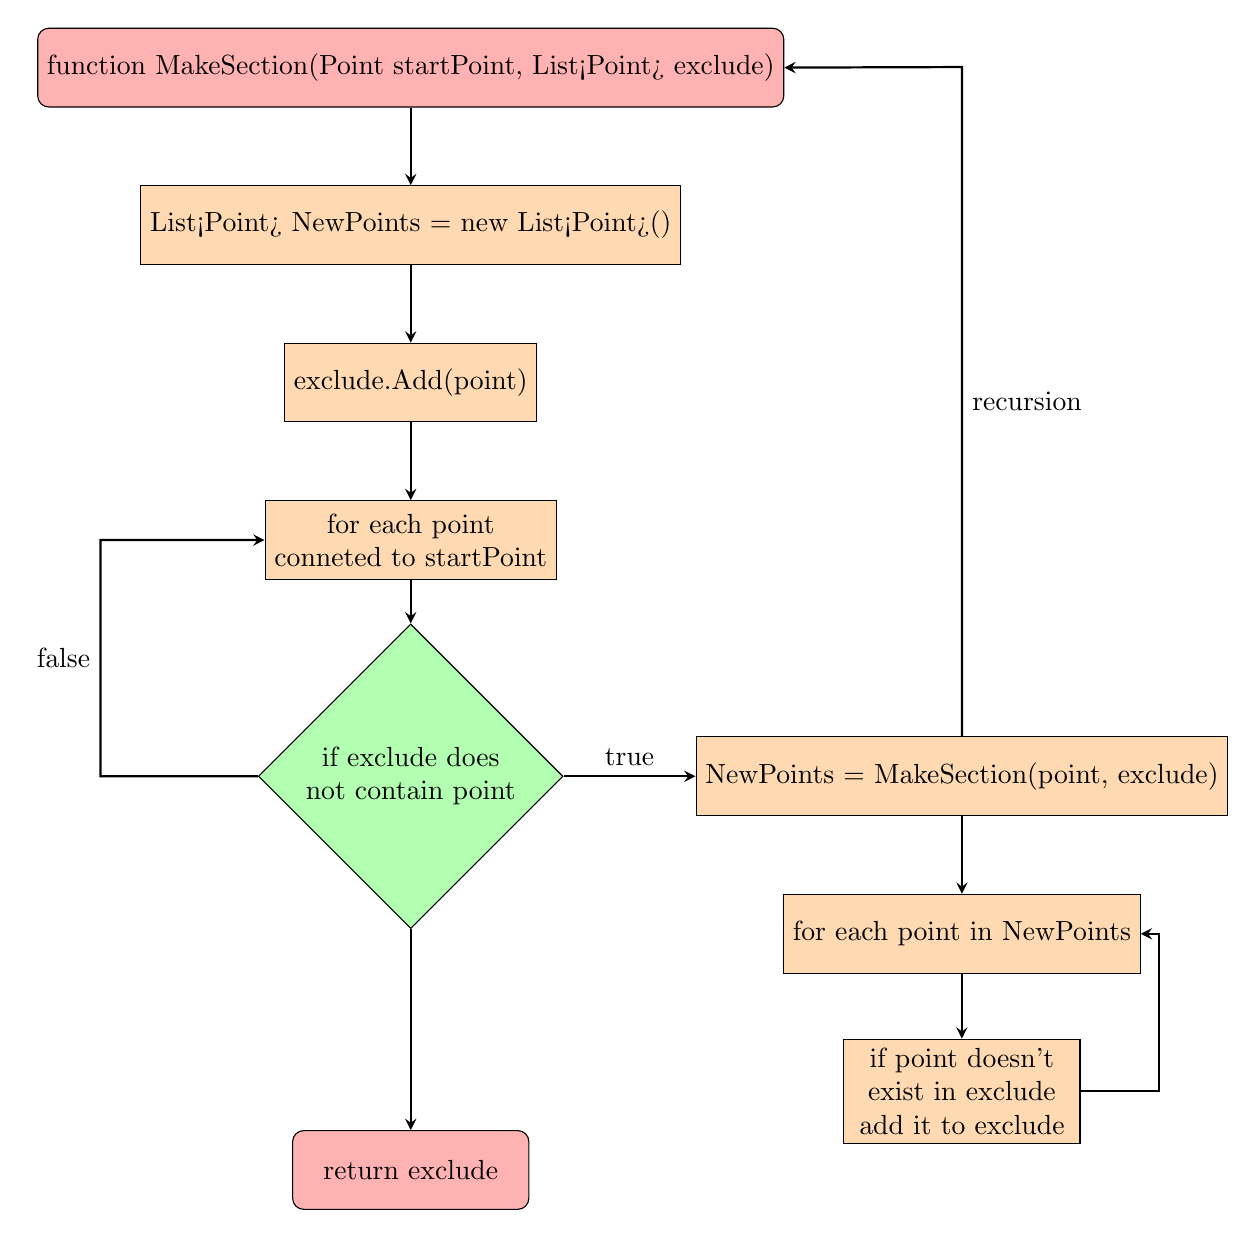
\begin{tikzpicture}[node distance=2cm,align=center]
    \node (start) [startstop] {function MakeSection(Point startPoint, List<Point> exclude)};
    \node (initpoints) [process, below of=start] {List<Point> NewPoints = new List<Point>()};
    \node (addexclude) [process, below of=initpoints] {exclude.Add(point)};
    \node (outerloop) [process, below of=addexclude] {for each point \\ conneted to startPoint};
    \node (checkexclude) [decision, below of=outerloop, yshift=-1cm] {if exclude does \\ not contain point};
    \node (branchout) [process, right of=checkexclude, xshift=5cm] {NewPoints = MakeSection(point, exclude)};
    \node (innerloop) [process, below of=branchout] {for each point in NewPoints};
    \node (addnewpoint) [process, below of=innerloop] {if point doesn't \\ exist in exclude \\ add it to exclude};
    \node (returnexclude) [startstop, below of=checkexclude, yshift=-3cm] {return exclude};
    
    \draw [arrow] (start) -- (initpoints);
    \draw [arrow] (initpoints) -- (addexclude);
    \draw [arrow] (addexclude) -- (outerloop);
    \draw [arrow] (outerloop) -- (checkexclude);
    \draw [arrow] (checkexclude) -- node[anchor=south] {true} (branchout);
    \draw [arrow] (checkexclude.west) -- ++(-2,0) -- node[anchor=east] {false} ++(0,3) -- (outerloop.west);
    \draw [arrow] (checkexclude.south) -- (returnexclude);
    \draw [arrow] (branchout) -- (innerloop);
    \draw [arrow] (branchout.north) -- node[anchor=west] {recursion} ++(0,8.5) -- (start.east);
    \draw [arrow] (innerloop) -- (addnewpoint);
    \draw [arrow] (addnewpoint.east) -- ++(1,0) |- (innerloop.east);
  \end{tikzpicture}
  \caption{Flowchart for recursive function to find entire section}
  \label{fig:recursive detect}
\end{figure}
\pagebreak

\textbf{Pseudocode for figure \ref{fig:recursive detect}} \linebreak
\textit{Recursive algorithm for detecting a section, given a starting point}
\begin{lstlisting}
function MakeSection(Point startPoint, List<Point> exclude)
List<Point> NewPoints = new List<Point>()
//add current startPoint to list of points to exclude
exclude.Add(point)
for each point in startPoint.Connectedpoints
{
	//branch out when point isn't already detected and is connected
	if exclude does not contain point
	{
		NewPoints = MakeSection(point, exclude)
		for each newPoint in NewPoints
		{
			if (newPoint doesn't exist in NewPoints)
			{
				exclude.Add(newPoint)
			}
		}
	}
}
return exclude
endfuntion
\end{lstlisting}

\myparagraph{Variable table}
\smallBr
\begin{tabular}{l|l|l}
Variable Name & Variable Type                      & Description                                              \\ \hline
point         & Point                              & Starting point for the algorithm to check                \\
exclude       & List\textless{}Point\textgreater{} & List of points to exclude when checking connected points \\
NewPoints     & List\textless{}Point\textgreater{} & Takes result of recursion in the algorithm              
\end{tabular}

\myparagraph{Identifying test data}
The algorithm will be successful if the following conditions are met:
\begin{itemize}
\item{An entire section is detected given a single input point}
\end{itemize}

\begin{figure}[p]
  \centering
  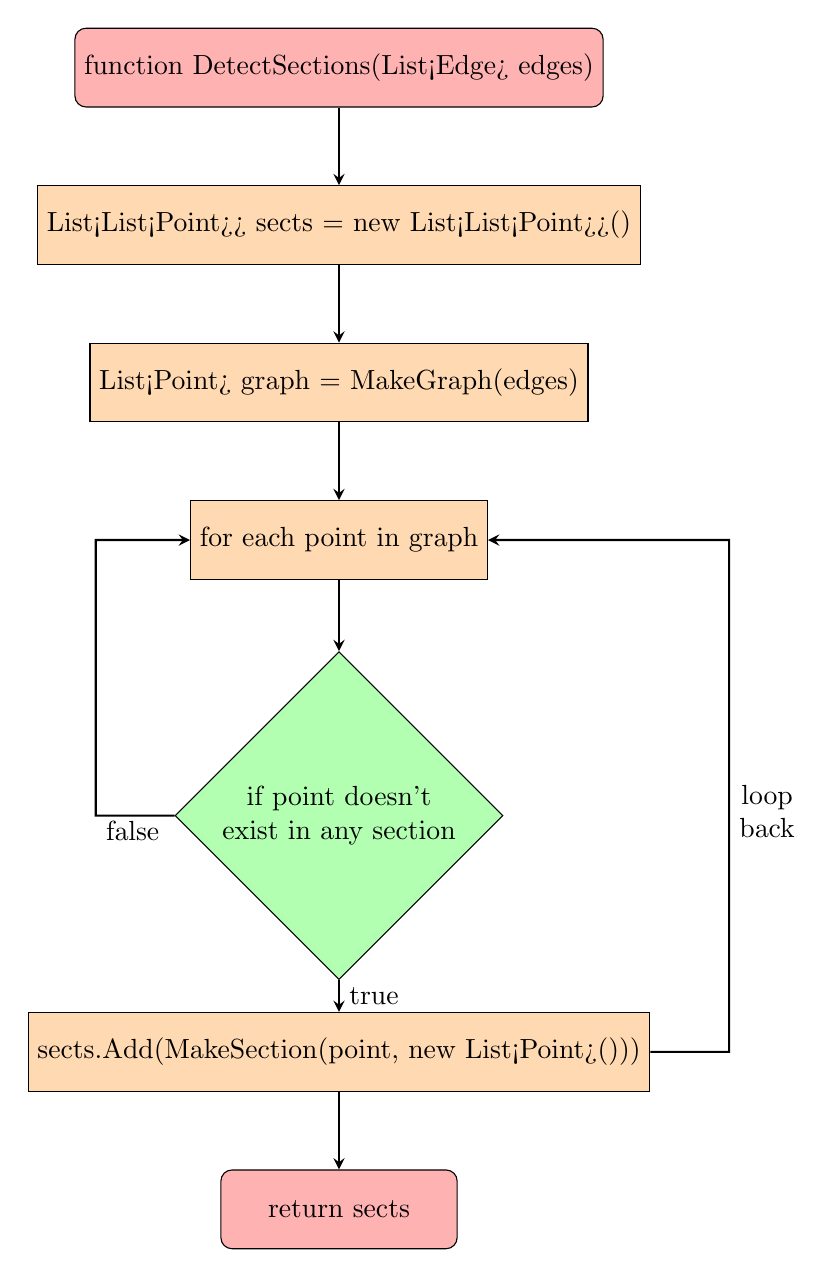
\begin{tikzpicture}[node distance=2cm, align=center]
    \node (start) [startstop] {function DetectSections(List<Edge> edges)};
    \node (initsects) [process, below of=start] {List<List<Point>> sects = new List<List<Point>>()};
    \node (initgraph) [process, below of=initsects] {List<Point> graph = MakeGraph(edges)};
    \node (outerloop) [process, below of=initgraph] {for each point in graph};
    \node (checkcondition) [decision, below of=outerloop, yshift=-1.5cm] {if point doesn't \\ exist in any section};
    \node (newsection) [process, below of=checkcondition, yshift=-1cm] {sects.Add(MakeSection(point, new List<Point>()))};
    \node (end) [startstop, below of=newsection] {return sects};
    
    \draw [arrow] (start) -- (initsects);
    \draw [arrow] (initsects) -- (initgraph);
    \draw [arrow] (initgraph) -- (outerloop);
    \draw [arrow] (outerloop) -- (checkcondition);
    \draw [arrow] (checkcondition) -- node[anchor=west] {true} (newsection);
    \draw [arrow] (checkcondition.west) -- ++(-1,0) node[anchor=west, yshift=-0.2cm] {false} -- ++(0,3.5) -- (outerloop.west);
    \draw [arrow] (newsection.east) -- ++(1,0) -- node[anchor=west, yshift=-0.2cm] {loop \\ back} ++(0,6.5) -- (outerloop.east);
    \draw [arrow] (newsection.south) -- (end);
  \end{tikzpicture}
  \caption{Flowchart for detecting if a new section needs to be made}
  \label{fig:detect-sections}
\end{figure}
\pagebreak

\textbf{Pseudocode for figure \ref{fig:detect-sections}} \linebreak
\textit{Algorithm for detecting weather a new section needs to be made given a list of edges}
\begin{lstlisting}
function DetectSections(List<Edge> edges)
//list of section, each section is a list of points
List<List<Point>> sects = new List<List<Point>>()
List<Point> graph = MakeGraph(edges)
for each point in graph
{
	check weather point already exists in sects
	
	if it doesn't exist start a new section with the not existing point as starting point
	{
		//add section to list of sections
		sects.Add(MakeSection(point, new List<Point>()))
	}
}
return sects
endfunction
\end{lstlisting}

\myparagraph{Variable table}
\smallBr
\begin{tabular}{l|l|l}
Variable Name & Variable Type                                                   & Description                                                                                                                                      \\ \hline
sections      & List\textless{}List\textless{}Point\textgreater{}\textgreater{} & Each List of points is an independent section                                                                                                    \\
graph         & List\textless{}Point\textgreater{}                              & List of points to be checked                                                                                                                     \\
edges         & List\textless{}Edge\textgreater{}                               & \begin{tabular}[c]{@{}l@{}}Gets turned into graph but is a parameter of the function since lists of edges\\ are easier to work with\end{tabular} \\
exist         & bool                                                            & Acts as a flag set to true if point already exists in a section                                                                                  \\
NewPoints     & List\textless{}Point\textgreater{}                              & Takes result of recursion in the algorithm                                                                                                      
\end{tabular}

\myparagraph{Identifying test data}
The algorithm will be successful if the following conditions are met:
\begin{itemize}
\item{Detects correct amount of sections}
\item{Doesn't create another section when point being checked is already in a section}
\end{itemize}

Now that I am able to detect sections we want to connect them. This is done by saving the list of edges from the triangulation section and finding the difference between the list after removing edges.

\begin{figure}[p]
  \centering
  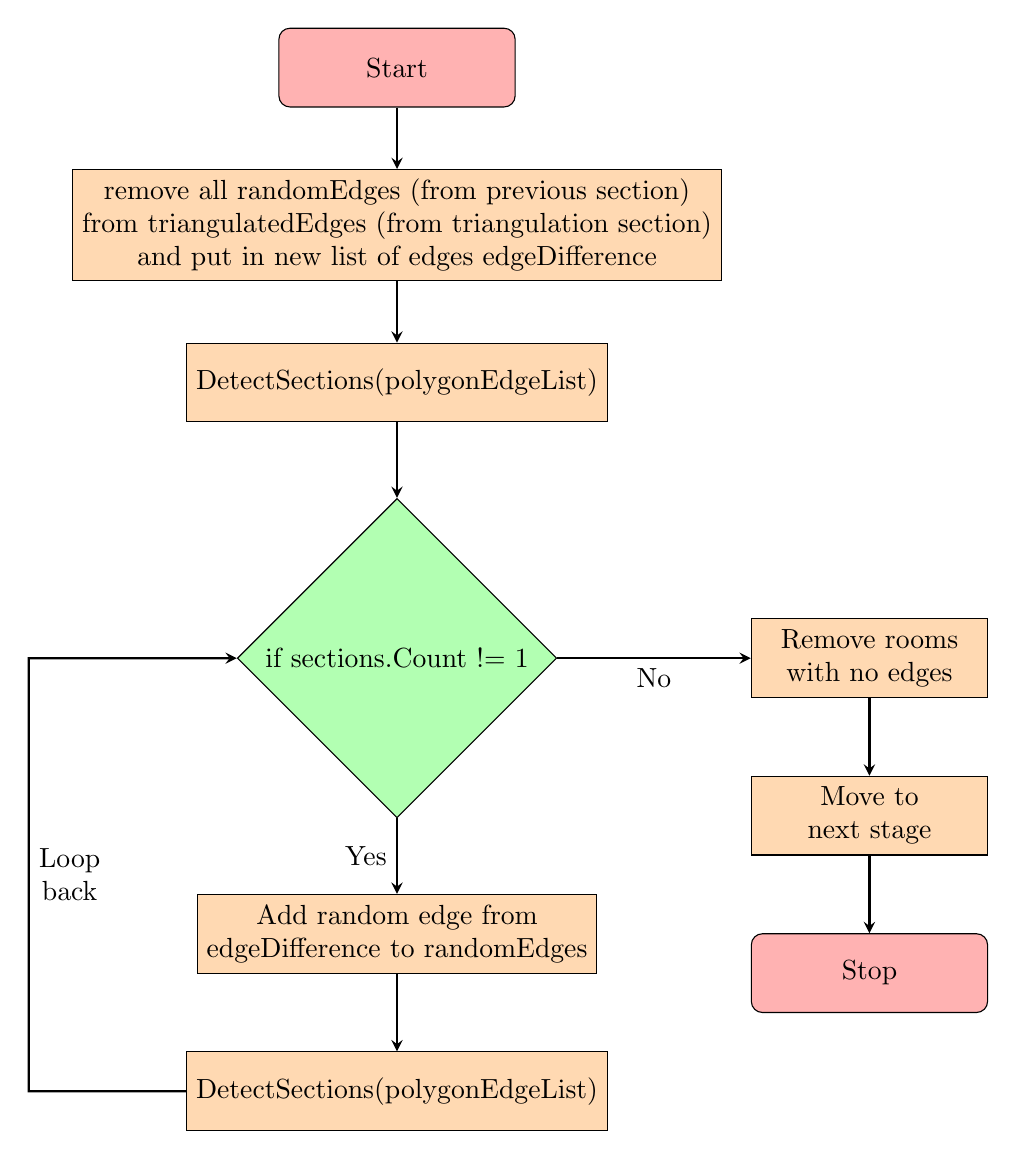
\begin{tikzpicture}[node distance=2cm, align=center]
    % Nodes
    \node (start) [startstop] {Start};
    \node (diff) [process, below of=start] {remove all randomEdges (from previous section) \\ from triangulatedEdges (from triangulation section) \\ and put in new list of edges edgeDifference};
    \node (detect) [process, below of=diff] {DetectSections(polygonEdgeList)};
    \node (decision) [decision, below of=detect, yshift=-1.5cm] {if sections.Count != 1};
    \node (addpoints) [process, below of=decision, yshift=-1.5cm] {Add random edge from \\ edgeDifference to randomEdges};
    \node (detect2) [process, below of=addpoints] {DetectSections(polygonEdgeList)};
    \node (removerooms) [process, right of=decision, xshift=4cm] {Remove rooms \\ with no edges};
    \node (nextstage) [process, below of=removerooms] {Move to \\ next stage};
    \node (stop) [startstop, below of=nextstage] {Stop};

    % Arrows
    \draw [arrow] (start) -- (diff);
    \draw [arrow] (diff) -- (detect);
    \draw [arrow] (detect) -- (decision);
    \draw [arrow] (decision) -- node[anchor=east] {Yes} (addpoints);
    \draw [arrow] (decision) -- node[anchor=north] {No} (removerooms);
    \draw [arrow] (addpoints) -- (detect2);
    \draw [arrow] (detect2.west) -- ++(-2,0) -- node[anchor=west] {Loop \\ back} ++(0,5.5) -- (decision);
    \draw [arrow] (removerooms) -- (nextstage);
    \draw [arrow] (nextstage) -- (stop);

  \end{tikzpicture}
  \caption{Flowchart for detecting sections in the program}
  \label{in game detect sections}
\end{figure}
\pagebreak


\textbf{Pseudocode for figure \ref{in game detect sections}}
\begin{lstlisting}
//code called once before main loop is started
//polygon is all the edge after triangulated
//polygonEdgeList are the edges left over after deleting a random amount
//polygonDifference is polygon - polygonEdgeList
List<Edge> polygonDifference(polygon, polygonEdgeList)
List<List<Point>> sections = DetectSections(polygonEdgeList)

//code inside the main loop that runs every frame
if (sections.Count != 1)
{
	//need to add points until there is only one section left
	int index = RandIntInRange(0,polygonDifference.Count - 1)
	//remove random edge from polygonDifference and add it to polygonEdgeList
	polygonEdgeList.Add(polygonDifference[index])
	polygonDifference.RemoveAtIndex(index)
	sections = DetectSections(polygonEdgeList)
}
else
{
	//remove rooms with no edges connected to them
	List<Point> graph = MakeGraph(polygonEdgeList)
	//all rooms are represented with an Area2D data type (custom structure made by godot) and need to check if children(the rooms) of the object are a point in the edgeList
	for each child in GetChildren
	{
		if (a point in graph doesn't have same position as a child)
		{
			//In this case the child isn't considered for in the edgeList
			RemoveChild(child)
		}
	}
	//move onto the next stage of generation
}
\end{lstlisting}

\myparagraph{Variable table}
\smallBr
\begin{tabular}{l|l|l}
Variable Name     & Variable Type                       & Description                                                                 \\ \hline
index             & int                                 & random number corresponding to index of edge to be added/removed                     \\
polygonEdgeList   & List\textless{}Edge\textgreater{}   & Edges left over after deleting, taken from previous section                                              \\
polygon           & List\textless{}Edge\textgreater{}   & All edges after triangulating                                               \\
polygonDifference & List\textless{}Edge\textgreater{}   & Whatever edges are left after polygon - polygonEdgelist                     \\
removeThese       & List\textless{}Area2D\textgreater{} & Collection of all rooms to be deleted since they don't have any connections
\end{tabular}

\myparagraph{Identifying test data}
The algorithm will be successful if the following conditions are met:
\begin{itemize}
\item{The list of edges are now all connected to each other}
\item{Removes all rooms without connections to other rooms}
\end{itemize}

\subsubsection{Turn edges into horizontal and vertical}
The movement system isn't optimised for edges that are angled in such obscure ways as seen in figure \ref{deleting edges result}. Therefore it's important to change the edges into it's vertical and horizontal components to make the level more traversable for the player. Originally I was going to create an advanced network to connect all the points in the most efficient way possible, but looking at how long it took me to implement delaunay triangulation I decided against it as it would take too long. So instead I created an algorithm that generates all possibilities to make sure all rooms are accessible.

\begin{figure}[h]
\centering
\includegraphics[width = 0.6\textwidth]{point possibilities}
\caption{All possibilities for points}
\label{point possibilities}
\end{figure}

The green dotted lines in figure \ref{point possibilities} shows where the new edges would be placed when they are replacing the old red edges. This does mean that each edge creates 4 new edges that will likely overlap with other edges, however once this is turned into a tilemap this isn't a problem as all these objects will be deleted.


\begin{figure}[p]
  \centering
  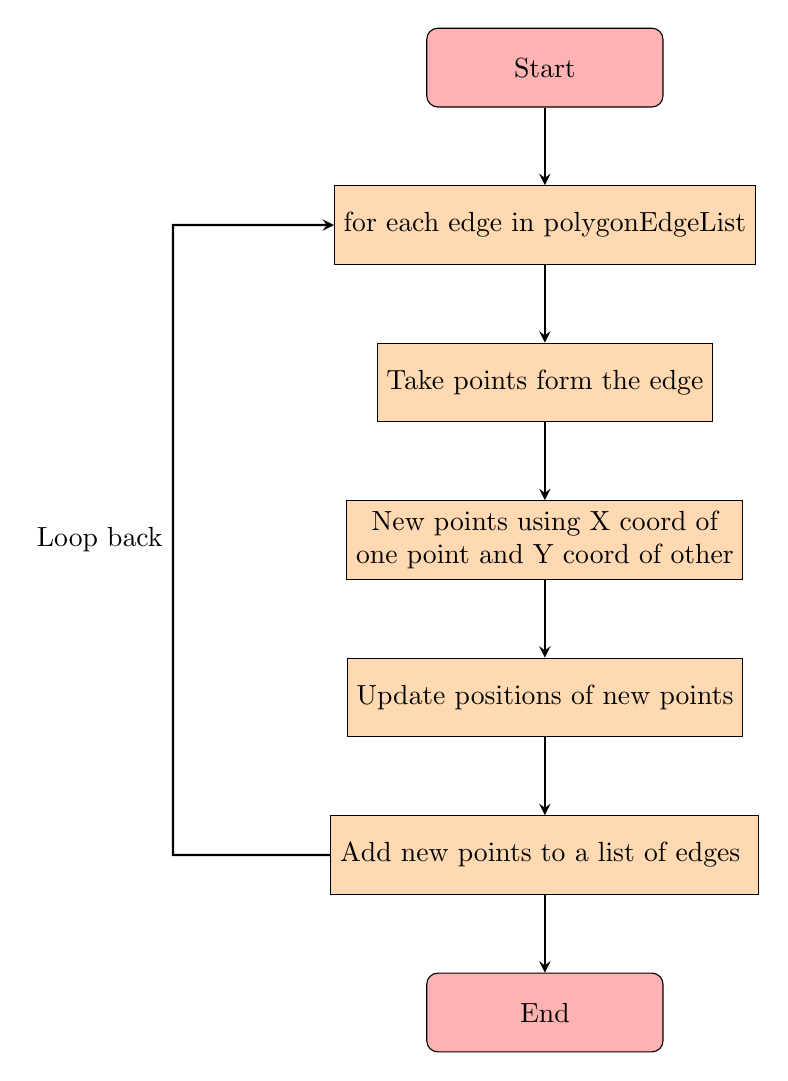
\begin{tikzpicture}[node distance=2cm, align=center]
    \node (start) [startstop] {Start};
    \node (forloop) [process, below of=start] {for each edge in polygonEdgeList};
    \node (getpoints) [process, below of=forloop] {Take points form the edge};
    \node (newpoints) [process, below of=getpoints] {New points using X coord of \\ one point and Y coord of other};
    \node (updatepoints) [process, below of=newpoints] {Update positions of new points};
    \node (addedges) [process, below of=updatepoints] {Add new points to a list of edges };
    \node (end) [startstop, below of=addedges] {End};
    
    \draw [arrow] (start) -- (forloop);
    \draw [arrow] (forloop) -- (getpoints);
    \draw [arrow] (getpoints) -- (newpoints);
    \draw [arrow] (newpoints) -- (updatepoints);
    \draw [arrow] (updatepoints) -- (addedges);
    \draw [arrow] (addedges.west) --++(-2,0) --++(0,8)  node[anchor=east, yshift=-4cm] {Loop back} -- (forloop.west);
    \draw [arrow] (addedges) -- (end);
  \end{tikzpicture}
  \caption{Flowchart for turning edges into horizontal and vertical edges}
  \label{fig:turn edges}
\end{figure}

\pagebreak


\textbf{Pseudocode for figure \ref{fig:turn edges}}
\begin{lstlisting}
polygon = new list of edges
//polygonEdgeList is a list of Edges from previous section
for each edge in polygonEdgeList
{
	//take position from points in edge in list
    Point point1 = edge.points[0];
    Point point2 = edge.points[1];
    //new temp point with no values
    Point newPoint1 = new Point(null);
    Point newPoint2 = new Point(null);
    newPoint1.AlterPos(new Vector2(point1.position.X, point2.position.Y));
    newPoint2.AlterPos(new Vector2(point2.position.X, point1.position.Y));
    //all possible paths made and stored in new list of edges (polygon)
    polygon.Add(new Edge(point1, newPoint1));
    polygon.Add(new Edge(point2, newPoint1));
    polygon.Add(new Edge(point1, newPoint2));
    polygon.Add(new Edge(point2, newPoint2));
}
\end{lstlisting}

\myparagraph{Variable table}
\smallBr
\begin{tabular}{l|l|l}
Variable Name   & Variable Type                     & Description                                                 \\ \hline
polygon         & List\textless{}Edge\textgreater{} & Contaings all the new edges generated                       \\
polygonEdgeList & List\textless{}Edge\textgreater{} & List of edges from the previous section                     \\
point1          & Point                             & First point of edge being checked                           \\
point2          & Point                             & Second point of edges being checked                         \\
newPoint1       & Point                             & End point for new edge after being made horizontal/vertical \\
newPoint2       & Point                             & End point for new edge after being made horizontal/vertical
\end{tabular}

\myparagraph{Identifying test data}
The algorithm will be successful if the following conditions are met:
\begin{itemize}
\item{Entire graph is made from horizontal and vertical edges}
\end{itemize}

In figure \ref{ba coridoors and edges} the pink lines are the edges before the rooms were generated. The green boxes are the result of this algorithm plus the generate corridors algorithm but it shows the algorithm well so it's included in this section.

\subsubsection{Generate corridors}
The edges currently have no depth as they are just a connection between two point so we need to convert it into something with an area that the player can interact with. Since we already have the edge we can iterate through the list of edges generated in the previous section and generate a corridor for each edge.

\begin{figure}[h]
    \centering
    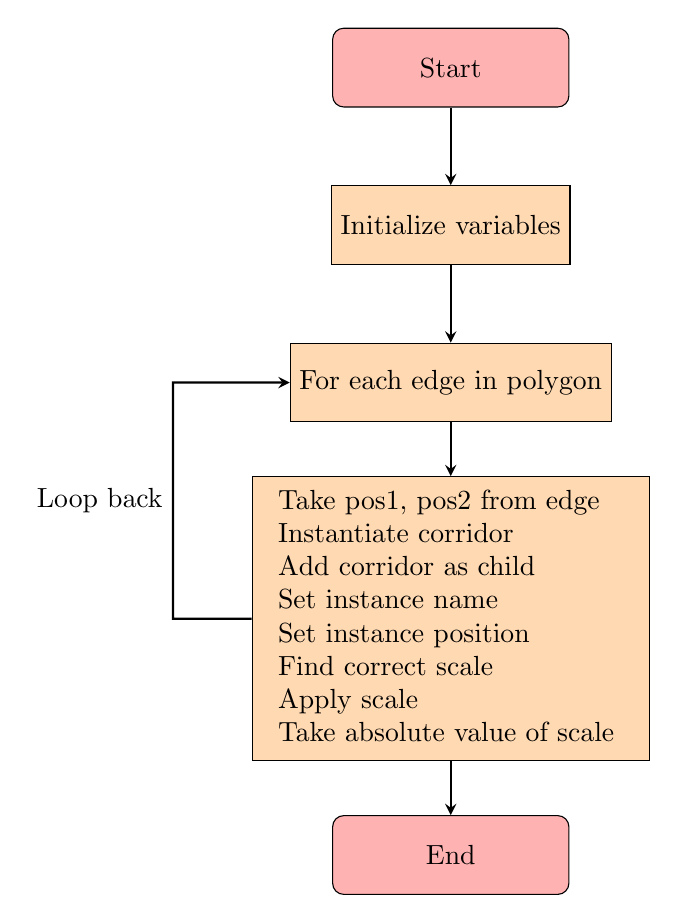
\begin{tikzpicture}[node distance=2cm, auto, align=center]
        % Nodes
        \node (start) [startstop] {Start};
        \node (init) [process, below of=start] {Initialize variables};
        \node (loop) [process, below of=init] {For each edge in polygon};
        \node (calculate) [process, below of=loop, yshift = -1cm] {
            \begin{tabular}{l}
                Take pos1, pos2 from edge \\
                Instantiate corridor \\
                Add corridor as child \\
                Set instance name \\
                Set instance position \\
                Find correct scale \\
                Apply scale \\
                Take absolute value of scale
            \end{tabular}
        };
        \node (end) [startstop, below of=calculate, yshift=-1cm] {End};

        % Arrows
        \draw [arrow] (start) -- (init);
        \draw [arrow] (init) -- (loop);
        \draw [arrow] (loop) -- (calculate);
        \draw [arrow] (calculate) -- (end);
        \draw [arrow] (calculate.west) -- ++(-1,0) -- node[anchor=east] {Loop back}  ++(0,3) -- (loop);

    \end{tikzpicture}
    \caption{Flowchart for the given pseudocode}
    \label{generate coridoor}
\end{figure}

\pagebreak

\textbf{Pseudocode for figure \ref{generate coridoor}} \linebreak
\textit{The result of this algorithm can be seen if figure \ref{ba coridoors and edges}}
\begin{lstlisting}
// polygon is edge list from previous section
// coridoorRadius is the radius of the coridoor as a vector2
for each edge in polygon
{
	//need to make corridor between two positions
    Vector2 pos1 = edge.points[0].position;
    Vector2 pos2 = edge.points[1].position;
    Node instance;
    instance = coridoor.Instantiate();
    AddChild(instance);
    //make sure they are tagged so that they can be recognised later
    instance.Name = "cr" + i;
    //place in middle
    instance.Position = (pos1 + pos2) / 2;
    //make sure the radius is added to right part of the room
    //want to add radius to bottom left of one point and top right of other
    Find correct scale and apply to instance
    Take absolute value of x and y of instance scale so it's always positive;
}
\end{lstlisting} 

\myparagraph{Variable table}
\smallBr
\begin{tabular}{l|l|l}
Variable Name & Variable Type                     & Description                                            \\ \hline
polygon       & List\textless{}Edge\textgreater{} & list of edges to be turned into coridoors              \\
edge          & Edge                              & The current edge being turned into a coridoor          \\
pos1          & Vector2                           & The start position of the coridoor                     \\
pos2          & Vector2                           & The end position of the coridoor                       \\
roomRadius    & Vector2                           & How much the coridoor corner is offset from the center \\
instance      & Node                              & The new coridoor that is instantiated                 
\end{tabular}

\myparagraph{Identifying test data}
The algorithm will be successful if the following conditions are met:
\begin{itemize}
\item{Each edge has a corridor generated for it}
\item{The corridor is an appropriate size}
\end{itemize}

However these rooms are still areas  that are solid blocks meaning that the player still isn't able to interact with any of the rooms as they are currently all solid blocks. That is why we need to regenerate the entire map to make it playable. A lot of the corridors are overlapping which could be problematic in the future however it wouldn't be worth it to remake that section as it would be very time consuming and wouldn't make any difference to the player since they would never see this section and would hardly effect the following sections.



\subsubsection{Turn into tile map}
Now that there is a large amount of rooms and corridors there needs to be a way of turning these areas into some kind of environment that the player can interact with. This can be done by turning the map into a tilemap, where the entire map is made of individual square tiles that the player can interact with. This is beneficial as it removes a lot of the detail the areas provide which makes it easier to manage. 

\begin{figure}[p]
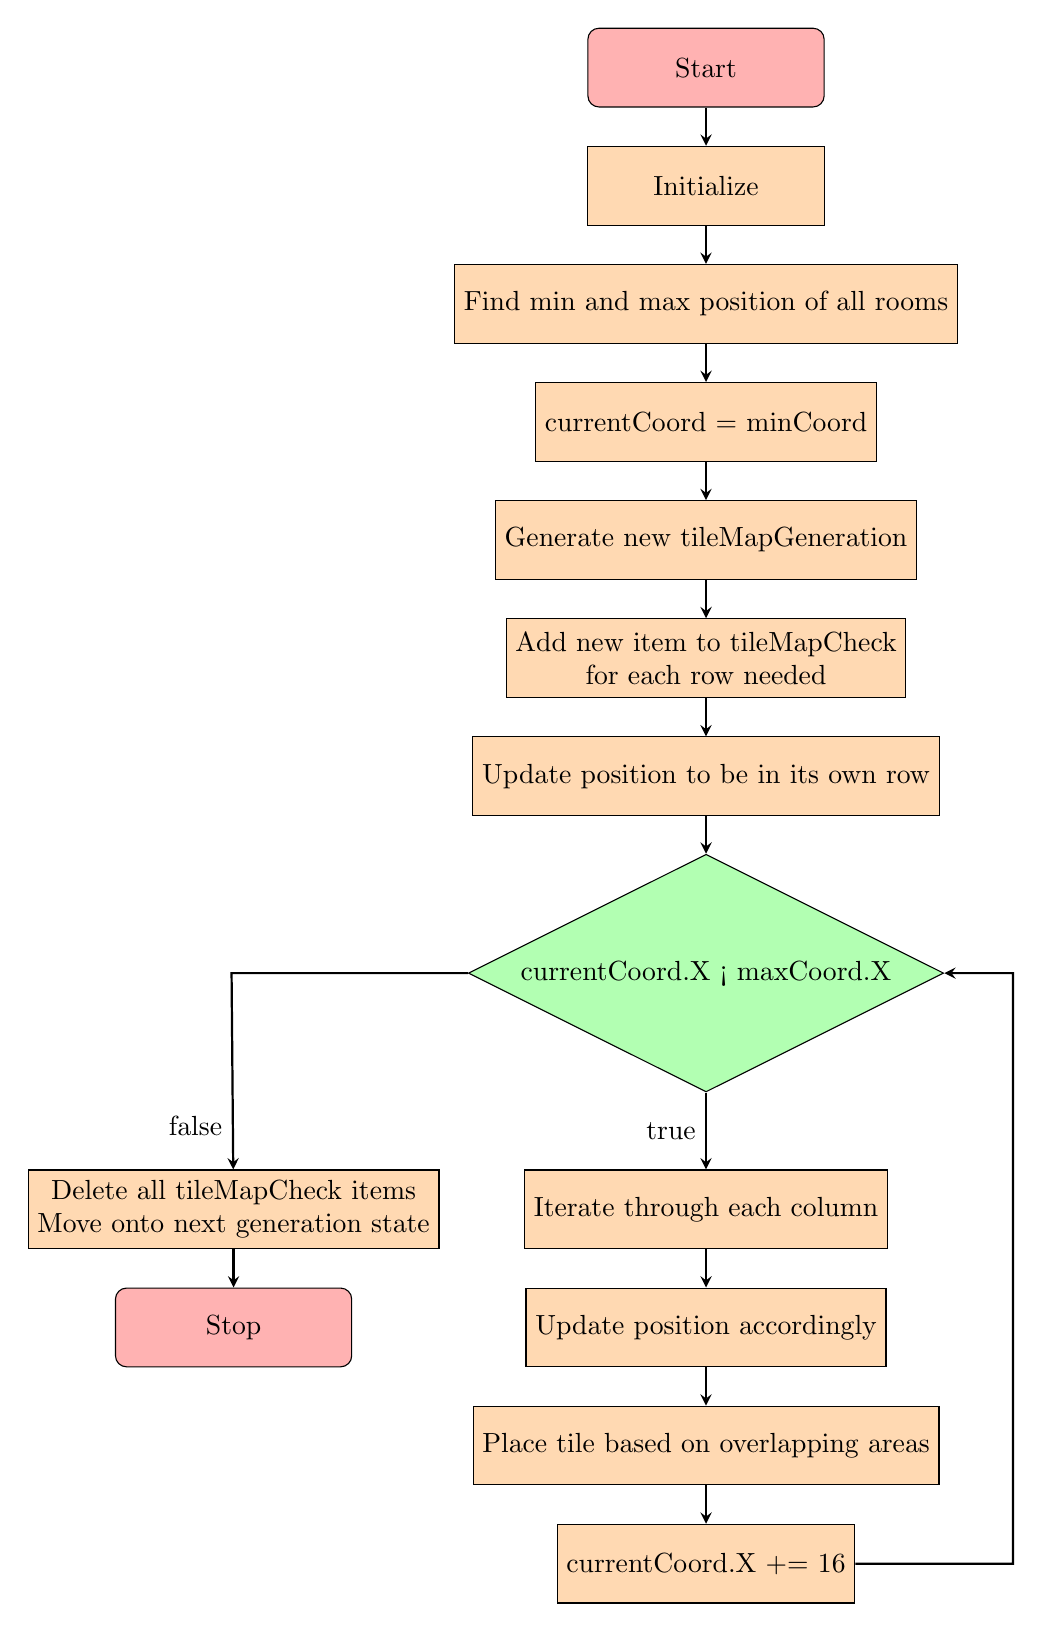
\begin{tikzpicture}[node distance=1.5cm, align=center]

\node (start) [startstop] {Start};
\node (init) [process, below of=start] {Initialize};
\node (minmax) [process, below of=init] {Find min and max position of all rooms};
\node (currentCoord) [process, below of=minmax] {currentCoord = minCoord};
\node (generate) [process, below of=currentCoord] {Generate new tileMapGeneration};
\node (addToCheck) [process, below of=generate] {Add new item to tileMapCheck \\ for each row needed};
\node (updatePosition) [process, below of=addToCheck] {Update position to be in its own row};
\node (iterate) [decision, below of=updatePosition, aspect=2, yshift=-1cm] {currentCoord.X < maxCoord.X};
\node (innerLoop) [process, below of=iterate, yshift=-1.5cm] {Iterate through each column};
\node (updateInnerPos) [process, below of=innerLoop] {Update position accordingly};
\node (placeTile) [process, below of=updateInnerPos] {Place tile based on overlapping areas};
\node (updateCoord) [process, below of=placeTile] {currentCoord.X += 16};
\node (else) [process, left of=iterate, xshift=-4.5cm, yshift=-3cm] {Delete all tileMapCheck items \\ Move onto next generation state};
\node (stop) [startstop, below of=else] {Stop};

\draw [arrow] (start) -- (init);
\draw [arrow] (init) -- (minmax);
\draw [arrow] (minmax) -- (currentCoord);
\draw [arrow] (currentCoord) -- (generate);
\draw [arrow] (generate) -- (addToCheck);
\draw [arrow] (addToCheck) -- (updatePosition);
\draw [arrow] (updatePosition) -- (iterate);
\draw [arrow] (iterate) -- node[anchor=east] {true} (innerLoop);
\draw [arrow] (innerLoop) -- (updateInnerPos);
\draw [arrow] (updateInnerPos) -- (placeTile);
\draw [arrow] (placeTile) -- (updateCoord);
\draw [arrow] (updateCoord.east) -- ++(2,0) -- ++(0,7.5) -- (iterate.east);
\draw [arrow] (iterate.west) -- ++(-3,0) -- node[anchor=east,yshift=-0.69cm] {false} (else);
\draw [arrow] (else) -- (stop);

\end{tikzpicture}
\caption{Flowchart for generating the tilemap}
\label{fc generating tilemap}
\end{figure}
\pagebreak

\textbf{Pseudocode for figure \ref{fc generating tilemap}} \linebreak
\textit{*one tile is 16 pixels large}
\begin{lstlisting}
//tileMapGeneration is a class containing properties that help decide what tile should be selected
tileMapCheck is a list of tileMapGeneration
Find min and max position of all rooms
currentCoord = minCoord;
//Find how much rows of tilemap are needed to make tilemap
checkAmount = (int)Mathf.Ceil((maxCoord.Y - minCoord.Y) / 16);
Node tempNode;
for (int i = 0; i < checkAmount; i++)
{
	//instantiate new Area2D that will check an area of the map
    tempNode = tileMapCheckScene.Instantiate();
    AddChild(tempNode);
    //update position so it's in it's own row
    tempNode.Position = currentCoord + new Vector2(0f, 16f * i);
    tileMapCheck.Add(tempNode);
}

//this part is ran every frame until next stage is reached
//iterate through each column
if (currentCoord.X < maxCoord.X)
{
    //check each box
    for (int i = 0; i < tileMapCheck.Count(); i++)
    {
        //update position accordingly
        tileMapCheck[i].area.Position = currentCoord + new Vector2(0f, 16f * i);
        place tile based on overlapping areas 
    }
    currentCoord.X += 16f;
}
else
{
    delete all tileMapCheck items
    move onto next generation state
}
\end{lstlisting}

\myparagraph{Variable table}
\smallBr
\begin{tabular}{l|l|l}
Variable Name     & Variable Type                                  & Description                                                                                                                      \\ \hline
tileMapCheck      & List\textless{}TileMapGeneration\textgreater{} & \begin{tabular}[c]{@{}l@{}}Contains all the areas that check what type of tile belongs in \\ what position\end{tabular}          \\
minCoord          & Vector2                                        & Minimum coordinate the tilemap will be generated                                                                                 \\
maxCoord          & Vector2                                        & Maximum coordinate the tilemap will be generated                                                                                 \\
currentCoord      & Vector2                                        & The current coordinate being checked                                                                                             \\
checkAmount       & integer                                        & The amount of tileMapCheck items to be created                                                                                   \\
tempNode          & Node                                           & \begin{tabular}[c]{@{}l@{}}Instantiates a scene so it can be used in the constructor \\ method of TileMapGeneration\end{tabular} \\
tileMapCheckScene & PackedScene                                    & The scene that is instantiated into tempNode                                                                                     \\
tilemap           & Tilemap                                        & The subject which has tiles generated into it                                                                                   
\end{tabular}

\myparagraph{Identifying test data}
The algorithm will be successful if the following conditions are met:
\begin{itemize}
\item{Takes reasonable amount of time}
\item{Variation in tiles that looks good}
\item{Makes an interesting map for the player to explore}
\end{itemize}

\subsubsection{Spawn player}
The only thing left is to let the player explore the map and battle the enemies for themselves. To do this we need to load the player object and place them into the spawn room.

\begin{figure}[h]
    \centering
    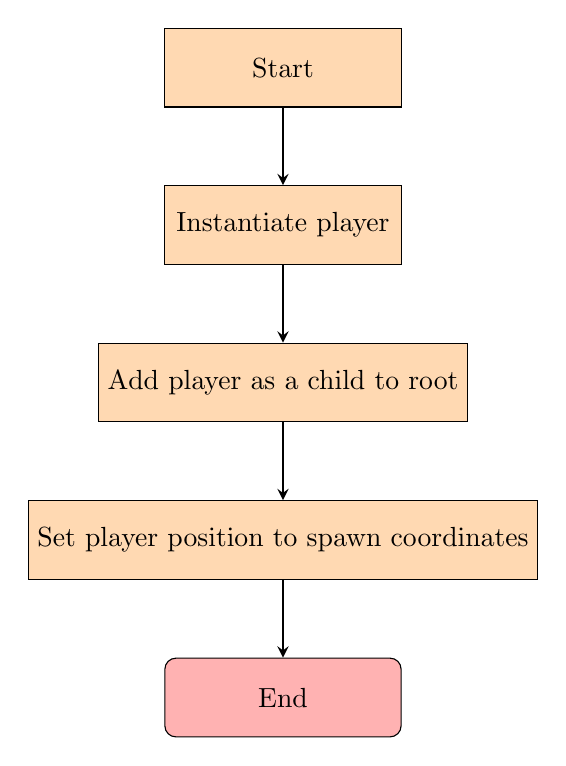
\begin{tikzpicture}[node distance=2cm, align=center]
    \node (start) [process] {Start};
    \node (instantiate) [process, below of=start] {Instantiate player};
    \node (addchild) [process, below of=instantiate] {Add player as a child to root};
    \node (putplayer) [process, below of=addchild] {Set player position to spawn coordinates};
    \node (end) [startstop, below of=putplayer] {End};
    
    \draw [arrow] (start) -- (instantiate);
    \draw [arrow] (instantiate) -- (addchild);
    \draw [arrow] (addchild) -- (putplayer);
    \draw [arrow] (putplayer) -- (end);
    
    \end{tikzpicture}
    \caption{Flowchart for spawning the player}
    \label{fig:spawn player}
\end{figure}

\textbf{Pseudocode for figure \ref{fig:spawn player}}
\begin{lstlisting}
Instantiate player
//Add child to root rather than temporary node holding all the area rooms
GetNode("/root").AddChild(player);
//Put player in spawn room
player.Position = spawnCoords;
\end{lstlisting}

\myparagraph{Variable table}
\smallBr
\begin{tabular}{l|l|l}
Variable Name  & Variable Type & Description                                                         \\ \hline
characterScene & PackedScene   & The scene which contains the player object                          \\
spawnCoords    & Vector2       & Position where player should be placed, taken form previous section
\end{tabular}

\myparagraph{Identifying test data}
The algorithm will be successful if the following conditions are met:
\begin{itemize}
\item{Player is spawned}
\item{Player is able to be controlled}
\end{itemize}

The player is now able to move around and explore the dungeon however we still need to design the player along with all of it's movement.

\subsection{Player Movement}

\subsection{Player Combat}
At this point in design I don't have enough time to create a proper combat system therefore this will be heavily reduced compared to the initial vision for this part.

\subsection{Enemy Design}

\subsection{Boss Design}

\subsection{UI}

\section{Developing a solution}
Since I am using the Godot game engine to create my project I can use many different languages which are supported in Godot such as C, C++, C\#, GDScript (made specifically for Godot) and other languages which were implemented by the community, using one of these languages would also mean that there would be less support, since less people would be using it and since it's not official the quality of the documentation may not be of the best quality. Therefore I have decided to use C\# to generate my project since I have the most experience with the language due to my experience with unity, however my knowledge is very limited and I would need to adapt my knowledge so I can apply it to Godot. 

\subsection{Dungeon Generation}
Each section will need to be completed for the algorithm to be finished, however each section may need multiple frames to be completed so to reliably switch between the generation states, for this to occur I created an enum variable and created an instance of the enum variable which can store one state defined in the enum variable. Below is an example of this in practice.
\begin{lstlisting}
//When initialising variables
private enum generationState
    {
        generationState1,
        generationState2,
        generationState3,
        generationState4,
        generationState5,
        finished
    }
private generationState currentState = generationState.generationState1;

//Code executing every frame
if (currnetState == generationState.generationState1)
{
	//Code for current section
}
else if (currnetState == generationState.generationState2)
{
	//Code for current section
}
else if (currnetState == generationState.generationState3)
{
	//Code for current section
}
else if (currnetState == generationState.generationState4)
{
	//Code for current section
}
else if (currnetState == generationState.generationState5)
{
	//Code for current section
}
\end{lstlisting}
This system was implemented later in development but it seems most appropriate in this part as it shows how I am able to switch from one generation state to another. It allows me to switch between states as I please since all I have to do is update the currentState variable. However in my case I just switch from one state to the next since once a section of code is executed it doesn't need to be revisited, if I do need to revisit code I made it into it's own function as it's more convenient.
\subsubsection{Create rooms}
\myparagraph{iteration 1}
The first iteration was made without the system for switching between generation stages.
\begin{lstlisting}
// presets for generating rooms
private int amountOfRooms = 100;
private float maxXScale = 20f;
private float minXScale = 8f;
private float maxYScale = 20f;
private float minYScale = 8f;
private int amountOfRooms = 50;

public override void _Ready()
{
    var rng = new RandomNumberGenerator();
    rng.Randomize();
    var room = GD.Load<PackedScene>("res://Scenes/room_generator.tscn");

    for (int i = 0; i < amountOfRooms; i++) //makes a certain amount of "rooms"
    {
    	    //Make room instance
        var instance = room.Instantiate();
        AddChild(instance);
        //Give random scale and position
        instance.GetNode<CollisionShape2D>("Collision").Scale = new Vector2(Map(rng.Randf(),minXScale,maxXScale), Map(rng.Randf(), minYScale, maxYScale)); //generates random scale
        instance.GetNode<Area2D>(".").Position = new Vector2(rng.Randf()*10, rng.Randf())*10; //generates initial random position
    }
    SpreadRooms();
}
\end{lstlisting}

\myparagraph{Iteration 2}
The last iteration set the position of each room to be a coordinate of two numbers between 0 and 1. This is inefficient because the rooms need to be spread apart so I could just spawn them further apart from each other so they have less distance to travel.

\parBr

I also changes the rooms from a cube with random scale to a pre-made room which can be instantiated as needed. In the future I will need to make more room variations to make it more interesting for the player. 

\parBr

Putting the code in the ready function means that it's called one before the game loads, with this all the rooms can be created before the game loads and they will be available to use once the scene is ready. Even if it takes a long time to load the scene all the rooms will be loaded when the rest of the generation starts. Which is crucial for the program to work.
\begin{lstlisting}
private int amountOfRooms = 25;
public override void _Ready()
{
	room = GD.Load<PackedScene>("res://Scenes/RoomVars/room_var_1.tscn");
	spreadFactor = amountOfRooms * 5f;
	for (int i = 0; i < amountOfRooms; i++) //makes a certain amount of "rooms"
	{
    	var instance = room.Instantiate();
    	AddChild(instance);
    	instance.GetNode<Area2D>(".").Position = new Vector2(rng.Randf() * spreadFactor, rng.Randf() * spreadFactor); //generates initial random position
	}
}
\end{lstlisting}

\myparagraph{Iteration 3}
For this iteration I aimed to add another room variation and because of this I would be able to scale this up for any amount of rooms I plan to add in the future
\begin{lstlisting}
private int amountOfRooms = 20;
public override void _Ready()
{
    rng.Seed = 00;
    rng.Randomize();  
    room1 = GD.Load<PackedScene>("res://Scenes/RoomVars/room_var_1.tscn");
    room2 = GD.Load<PackedScene>("res://Scenes/RoomVars/room_var_2.tscn");
    spreadFactor = amountOfRooms * 5f;
    int randNum;
    
    #region make rooms
    // Makes a certain amount of "rooms"
    for (int i = 0; i < amountOfRooms; i++)
    {
        Node instance;
        //pick random room variation
        randNum = rng.RandiRange(0, 1);
        if (randNum == 0)
        {
            instance = room1.Instantiate();
        }
        else if (randNum == 1)
        {
            instance = room2.Instantiate();
        }
        else
        {
        	//would never be called but needs to exist because without it there is a syntax error
            instance = room1.Instantiate();
        }
        AddChild(instance);
        // Generates initial random position
        instance.GetNode<Area2D>(".").Position = new Vector2((float)Math.Round(rng.Randf() * spreadFactor), (float)Math.Round(rng.Randf() * spreadFactor)); 
    }
    #endregion
}
\end{lstlisting}

\myparagraph{Iteration 4}
For this iteration I aimed to add more room variations and make it even easier to add more variations if needed in the future, since one of the stakeholders has said that they would like there to be a variation in the rooms, so that each room doesn't feel the same.
\begin{lstlisting}
private int amountOfRooms = 50;
private Vector2 scaleRange = new Vector2(1f, 1.5f); //min and max of scalse of rooms
private int roomVars = 10;
public override void _Ready()
{
    rng.Seed = 00;
    rng.Randomize(); 
    float spreadFactor = amountOfRooms * 10f;
    int randNum;
    float scaleRand;
    
    #region make rooms
    //Load all the scenes with the room variations
    Node instance;
    List<PackedScene> rooms = new List<PackedScene>();
    for (int i = 0; i < roomVars; i++)
    {
        rooms.Add(GD.Load<PackedScene>("res://Scenes/RoomVars/room_var_" + i + ".tscn"));
    }
	//Instantiate a random room variation
    for (int i = 0; i < amountOfRooms; i++) // Makes a certain amount of "rooms"
    {
        randNum = rng.RandiRange(0, roomVars - 1);
        instance = rooms[randNum].Instantiate();
        //label room for identification later
        instance.Name = ("rm" + i);
        AddChild(instance);
		//Add some variation to the size of the rooms
        scaleRand = rng.RandfRange(scaleRange.X, scaleRange.Y);
		//flip room variation so that it appears there are more room variations
        if (rng.RandiRange(0, 1) == 0)
        {
            scaleRand *= -1;
        }
		// Generates initial random position and scale
        instance.GetNode<Area2D>(".").Scale = new Vector2(scaleRand, scaleRand);
        instance.GetNode<Area2D>(".").Position = new Vector2(Mathf.Round(rng.Randf() * spreadFactor * 3f), Mathf.Round(rng.Randf() * spreadFactor)); 
    }
    #endregion
}
\end{lstlisting}
This iteration allows me to use a naming convention to add all the scenes to a list and then instantiate a room from that list. This satisfies all the needs for development in the future and further generation states, therefore it's complete.

\subsubsection{Spread rooms}
\myparagraph{Iteration 1}
C\# offers an async function which allows me to run the code while other things are happening, by dedicating a thread to this task. This allows the while loop to work since the code is executed until an end condition is met.
\begin{lstlisting}
//spreading rooms apart
private bool spread = false;
private int count = 0;
private Vector2 direction = Vector2.Zero;
private float step = 1f;
//temp statistics stuff for testing
private int loopCount = 0;

public async void SpreadRooms()
{
    //this only runs once at the start of the game so the inefficiency is loading time
    while (!spread) //if the rooms have overlapping areas
    {
        loopCount += 1;
        step = 2 + (4000/(((0.1f*MathF.Pow(loopCount,2f))+200)));
        await Task.Delay(TimeSpan.FromMilliseconds(1));
        count = 0; //resets count to check overlapping areas of child
        for (int i = 0; i < amountOfRooms; i++)
        {
            if (GetChild<Area2D>(i).HasOverlappingAreas()) //if there are overlapping areas on the child
            {
                direction = Vector2.Zero; //resets direction to 0
                for (int j = 0; j < GetChild<Area2D>(i).GetOverlappingAreas().Count; j++) //check every overlapping area
                {
                    direction += GetChild<Area2D>(i).Position - GetChild<Area2D>(i).GetOverlappingAreas()[j].Position; //finds difference between original area and overlapping area
                }
                //changes area position
                direction = direction.Normalized();
                GetChild<Area2D>(i).Position += direction * step;
            }
            else
            {
                count += 1; //adds 1 to count if no overlapping areas
            }
        }
        if (count == amountOfRooms)
        {
            spread = true;
            GD.Print("fin");
            GD.Print(loopCount);
        }
    }
}
\end{lstlisting}
Using an async function would mess up my work flow since I am unable to switch between generation stages since one an async function has began it would be difficult to end the task and since I am using methods native to Godot, inside an async method the refresh rate between the two threads may not be aligned properly so checking overlapping areas would have no result until Godot has updated slowing the program down and it would most likely cause problems when other sections are introduced.

\myparagraph{Iteration 2}
This iteration moves the room one at a time rather than all of them one bit at a time. However it's inside the void which updates every frame, which will make it easier for managing sections.
\begin{lstlisting}
public override void _Process(double delta)
{
    if (currentState == generationState.spreadRooms)
    {
        for (int i = 0; i < GetChildCount(); i++)
        {
            Thread.Sleep(1);
            while (GetChild<Area2D>(i).HasOverlappingAreas())
            {
                Thread.Sleep(1);
                direction = Vector2.Zero; // Resets direction to 0
                for (int j = 0; j < GetChild<Area2D>(i).GetOverlappingAreas().Count; j++) 
                {
                	// Check every overlapping area
                    displacement = GetChild<Area2D>(i).Position - GetChild<Area2D>(i).GetOverlappingAreas()[j].Position;
                    direction += (10 / displacement.Length()) * displacement.Normalized(); 
                    // Finds difference between original area and overlapping area
                }
                //update position of room
                direction = direction.Normalized();
                GetChild<Area2D>(i).Position += direction * step;
            }
        }
        currentState = generationState.deleteRooms;
    }
    // Code for other sections (when it exists)
}
\end{lstlisting}
The problem with this is the fact that it uses a while loop, which is bad practice to start every frame. As it sometimes makes the program stop responding when running. Also the room sometimes gets stuck between other rooms as it keeps moving a room in an infinite loop since it's trying to move the rooms one at a time. This iteration still needs to use thread.sleep to slow the thread as too much processing happens per frame which causes the program to freeze, this will need to be expanded upon next iteration.

\myparagraph{Iteration 3}

\begin{lstlisting}
 public override void _Process(double delta)
    {
        if (currentState == generationState.spreadRooms)
        {
            #region spreading rooms
            count = 0; //resets count to check overlapping areas of child
            for (int i = 0; i < amountOfRooms; i++)
            {
                if (GetChild<Area2D>(i).HasOverlappingAreas()) //if there are overlapping areas on the child
                {
                    direction = Vector2.Zero; //resets direction to 0
                    for (int j = 0; j < GetChild<Area2D>(i).GetOverlappingAreas().Count; j++) //check every overlapping area
                    {
                        displacement = GetChild<Area2D>(i).Position - GetChild<Area2D>(i).GetOverlappingAreas()[j].Position;
                        direction += (10 / displacement.Length()) * displacement.Normalized(); //finds difference between original area and overlapping area
                    }
                    // Rounds the result to make the numbers easier to work with
                    direction = direction.Normalized() * step;
                    direction.X = Mathf.Round(direction.X) * step;
                    direction.Y = Mathf.Round(direction.Y) * step;
                    GetChild<Area2D>(i).Position += direction;
                }
                else
                {
                    count += 1; //adds 1 to count if no overlapping areas
                }
            }
            if (count == amountOfRooms)
            {
                currentState = generationState.deleteRooms;
                return;
                //GD.Print("fin");
                //GD.Print(loopCount);
            }
		}
		// Code for other sections (when it exists)
	}
\end{lstlisting}

\myparagraph{Iteration 4}
I implemented the switching of generation states using the enum variable. As well as taking the reciprocal of what the room needs to be displaced so that rooms closer to the room being checked will have more of an effect on the displacement, hopefully making the algorithm faster.
\begin{lstlisting}
public override void _Process(double delta)
{
    if (currentState == generationState.spreadRooms)
    {
        #region spreading rooms
        count = 0; 
        // Resets count to check overlapping areas of child
        for (int i = 0; i < amountOfRooms; i++)
        {
            // If there are overlapping areas on the child
            if (GetChild<Area2D>(i).HasOverlappingAreas()) 
            {
                direction = Vector2.Zero; // Resets direction to 0
                // Check every overlapping area
                for (int j = 0; j < GetChild<Area2D>(i).GetOverlappingAreas().Count; j++) 
                {
                    // Finds difference between original area and overlapping area
                    displacement = GetChild<Area2D>(i).Position - GetChild<Area2D>(i).GetOverlappingAreas()[j].Position;
                    // Take reciprocal so closer rooms have more of an effect
                    direction += (10 / displacement.Length()) * displacement.Normalized(); 
                }
                direction = direction.Normalized();
                GetChild<Area2D>(i).Position += direction * step * rng.Randf();
            }
            else
            {
                count += 1; // Adds 1 to count if no overlapping areas
            }
        }
        if (count == amountOfRooms)
        {
            // Move onto the next stage of generation
            spread = true;
            currentState = generationState.deleteRooms;
            return;
        }
        #endregion
    }
    // Code for other sections
}

\end{lstlisting}
The algorithm in it's current state allows for development in the future (if needed) since it's well commented, it also achieves it's purpose therefore it's complete. 

\subsubsection{Delete rooms}
\myparagraph{Iteration 1}
Algorithm generates a random index for a room to be deleted
\begin{lstlisting}
//Needs to be between 0-1 (if its 0.8 it will delete 80% of rooms)
private float deletingRoomsFactor = 0.5f; 
public override void _Process(double delta)
{
    // Code for other sections

    if (currentState == generationState.deleteRooms)
    {
        #region delete rooms
        for (int i = 0; i < (int)(amountOfRooms * deletingRoomsFactor); i++)
        {
        	//generate index of room to delete
            count = rng.RandiRange(0, GetChildCount());
            RemoveChild(GetChild<Area2D>(count));
        }
        currentState = generationState.triangulation;
        #endregion
    }

    // Code for other sections
}
\end{lstlisting}
Will error when count = GetChildCount() since there is nothing at that index as the last item of the list is GetChildCount()-1.

\myparagraph{Iteration 2}
Simple fix to improve last iteration
\begin{lstlisting}
//Needs to be between 0-1 (if its 0.8 it will delete 80% of rooms)
private float deletingRoomsFactor = 0.5f; 
public override void _Process(double delta)
{
    // Code for other sections

    if (currentState == generationState.deleteRooms)
    {
        #region delete rooms
        for (int i = 0; i < (int)(amountOfRooms * deletingRoomsFactor); i++)
        {
        	//generate index of room to delete
            count = rng.RandiRange(0, GetChildCount() -1);
            RemoveChild(GetChild<Area2D>(count));
        }
        currentState = generationState.triangulation;
        #endregion
    }

    // Code for other sections
}
\end{lstlisting}
The algorithm performs the task that it's required to do therefore the algorithm is complete

\subsubsection{Delaunay triangulation}
\myparagraph{Point Class iteration 1}
There is no advantage using the point class over just using a list of Area2D's yet, apart from accessing the position is slightly more convenient.
\begin{lstlisting}
class Point
{
    Area2D area;
    Vector2 position;

    public Point(Area2D area)
    {
    		//Constructor method for point
        this.area = area;
        //Position is for convenience
        position = area.Position;
    }
}
\end{lstlisting}
The attributes also aren't declared as public or private, by default C\# assumes that they are private so all the values aren't able to be updated since there are no methods to access them.

\myparagraph{Point Class iteration 2}
Changing the attributes to public allows me to access them from any other class in C\#, which may be bad practice but it performs the function that it needs to do.
\parBr
The AlterPos method was added so that the position of the point can be altered without actually changing the position of the area that the point represents. This is used for the superTri points in the delaunay triangulation function as they don't need to have an area, so the value is set to null, but their position is necessary for the algorithm to function.
\begin{lstlisting}
public class Point
{
    public Area2D area;
    public Vector2 position;

    public Point(Area2D area)
    {
        this.area = area;
        position = area.Position;
    }

    public void AlterPos(Vector2 newPos)
    {
    		//allows to update position without actually changing position of area
        position = newPos;
    }
}
\end{lstlisting}

\myparagraph{Point Class iteration 3}
To represent the points as a graph I would need to know which other points they are connected to so for this iteration I added a list of points of which the point is connected to, allowing me to represent rooms layout as a directed graph, once the triangulation has completed.
\begin{lstlisting}
public class Point
{
    // Point in a graph also represents a room in the code
    public Area2D area;
    public Vector2 position;
    public List<Point> connectedPoints = new List<Point>();

    public Point(Area2D Area)
    {
        area = Area;
		//For super triangle the points don't have area so null is passed in
        if (area == null)
        {
            position = new Vector2();
        }
        else
        {
            position = Area.Position;
        }
    }

    public void AlterPos(Vector2 newPos)
    {
        position = newPos;
    }
	//Want to do input validation on connected points so this method exists
    public void ConnectPoint(Point newPoint)
    {
        if (newPoint == null || newPoint.position == position || connectedPoints.Any(x => x.position == newPoint.position))
        {
        	//If newPoint doesn't exist or is the current point or is already connected.
        	//Want to know if this is called since if it gets called printed something went wrong
            GD.Print("Invalid point");
            return;
        }

        connectedPoints.Add(newPoint);
    }
}
\end{lstlisting}

\myparagraph{Edge Class iteration 1}
The edge aims to represent the connection between two points. The midpoint and perpendicular methods are used to help the triangle class to find the circumcentre and circumcircle of the triangle.
\begin{lstlisting}
class Edge
{
    public Point[] points = new Point[2]; // 2 points make an edge

    public Edge(Point point1, Point point2)
    {
        points[0] = point1;
        points[1] = point2;
        // Set the value of the two points
    }

    public Vector2 Midpoint()
    {
    		//Finds the midpoint of the two points
        Vector2 mid;
        mid.X = 0.5f * (points[0].position.X + points[1].position.X);
        mid.Y = 0.5f * (points[0].position.Y + points[1].position.Y);
        return mid;
    }

    public float Perpendicular()
    {
    		//finds perpendicular of gradient of line that links the two points
        float gradient = (points[0].position.X - points[1].position.X) / (points[0].position.Y - points[1].position.Y);
        return (-1f / gradient);
    }
}
\end{lstlisting}
Checking weather two edges are composed of the same points is problematic since C\# checks weather they are the same so comparing two edges may not work for all cases.


\myparagraph{Edge Class iteration 2}
This iteration adds the HasPoints method which allows me to check if two edges are the same or if an edge is composed of two specific points. This is useful as when comparing two edges, they could be made up of the same points however since they are different instances they wouldn't be considered as the same edge, for my use case I want to consider them as the same edge, this method allows me to accomplish this
\begin{lstlisting}
public class Edge
{
    public Point[] points = new Point[2]; // 2 points make an edge

    public Edge(Point point1, Point point2)
    {
        points[0] = point1; points[1] = point2; // Set value of the two points
    }

    public Vector2 midpoint() // Finds midpoint of edges
    {
        Vector2 mid;
        mid.X = 0.5f * (points[0].position.X + points[1].position.X);
        mid.Y = 0.5f * (points[0].position.Y + points[1].position.Y);
        return mid;
    }

    public float perpendicular() // Finds perpendicular gradient of the line that links the two points
    {
        float gradient = (points[0].position.X - points[1].position.X) / (points[0].position.Y - points[1].position.Y);
        return (-1f / gradient);
    }

    public bool HasPoints(Point point1, Point point2) // Checks whether the edge is composed of specified points
    {
        if ((points[0] == point1 && points[1] == point2) || (points[0] == point2 && points[1] == point1))
        {
            return true;
        }
        else
        {
            return false;
        }
    }
}
\end{lstlisting}

\myparagraph{Triangle Class iteration 1}
This class aims to bring together 3 edges and 3 points.
\begin{lstlisting}
class Triangle
{
    public Edge[] edges = new Edge[3]; // 3 edges make a triangle
    public Vector2 circumcentre;
    public float radius;

    public Triangle(Edge edge1, Edge edge2, Edge edge3)
    {
        edges[0] = edge1; edges[1] = edge2; edges[2] = edge3; // Set value of all the edges
        FindCircumcentre();
        FindRadius();
    }

    public bool IsWithin(Point newNode)
    {
        // Check whether the new node lies within the circumcircle
        // Doesn't exist yet
        return false;
    }

    private void FindCircumcentre()
    {
        // Find circumcentre of the circumcircle
        // Finds x coordinate of circumcentre
        circumcentre.X = ((edges[1].Midpoint().X * edges[1].Perpendicular()) - (edges[2].Midpoint().X * edges[2].Perpendicular()) + (edges[2].Midpoint().Y - edges[1].Midpoint().Y)) / (edges[1].Perpendicular() - edges[2].Perpendicular());

        // Finds y coordinate of circumcentre
        circumcentre.Y = (edges[2].Perpendicular() * (circumcentre.X - edges[2].Midpoint().X)) + edges[2].Midpoint().Y;
        //This doesn't work yet
    }

    private void FindRadius()
    {
        // Find radius of circumcircle that the edges lie on
        // Pythagorean theorem to find distance between points and centre
        radius = Mathf.Sqrt(MathF.Pow((circumcentre.X - edges[0].points[0].position.X), 2f) + MathF.Pow((circumcentre.Y - edges[0].points[0].position.Y), 2f));
    }
}

\end{lstlisting}

\myparagraph{Triangle Class iteration 2}
Equation used in the findCircumcentre method is taken from \cite{equation}. The method not also actually works and returns the correct result.
\begin{lstlisting}
public class Triangle
{
    public Edge[] edges = new Edge[3]; // 3 edges make a triangle
    public Point[] points = new Point[3];
    public Vector2 circumcentre;
    public float radius;

    public Triangle(List<Triangle> triangulation, Point point1, Point point2, Point point3)
    {
        points[0] = point1; points[1] = point2; points[2] = point3;

        #region edge check
        // Checks whether the edge already exists and if not, it creates a new one
        int edge1index = -1;
        int edge2index = -1;
        int edge3index = -1;

        for (int i = 0; i < triangulation.Count; i++)
        {
            if (triangulation[i].ContainsEdge(new Edge(point1, point2)) != null && edge1index == -1)
            {
                edge1index = i;
            }
            if (triangulation[i].ContainsEdge(new Edge(point2, point3)) != null && edge2index == -1)
            {
                edge2index = i;
            }
            if (triangulation[i].ContainsEdge(new Edge(point1, point3)) != null)
            {
                edge3index = i;
            }
        }

        if (edge1index != -1)
        {
            edges[0] = triangulation[edge1index].ContainsEdge(new Edge(point1, point2));
        }
        else
        {
            edges[0] = new Edge(point1, point2);
        }

        if (edge2index != -1)
        {
            edges[1] = triangulation[edge2index].ContainsEdge(new Edge(point2, point3));
        }
        else
        {
            edges[1] = new Edge(point2, point3);
        }

        if (edge3index != -1)
        {
            edges[2] = triangulation[edge3index].ContainsEdge(new Edge(point1, point3));
        }
        else
        {
            edges[2] = new Edge(point1, point3);
        }
        #endregion

        findCircumcentre();
        findRadius();
    }

    public Edge ContainsEdge(Edge edgeToCompare)
    {
        Point point1 = edgeToCompare.points[0];
        Point point2 = edgeToCompare.points[0];

        for (int i = 0; i < 3; i++)
        {
            if (edges[i].HasPoints(point1, point2))
            {
                return edges[i];
            }
        }

        return null;
    }

    public bool isWithin(Point newNode)
    {
        // Check whether the new node lies within the circumcircle
        // Pythagorean theorem to check if it lies within
        if (Mathf.Pow(newNode.position.X - circumcentre.X, 2f) + Mathf.Pow(newNode.position.Y - circumcentre.Y, 2f) < MathF.Pow(radius, 2f))
        {
            return true;
        }
        else
        {
            return false;
        }
    }

    private void findCircumcentre()
    {
        // Find circumcentre of the circumcircle
        // Equation from https://www.omnicalculator.com/math/circumcenter-of-a-triangle
        float t = Mathf.Pow(points[0].position.X, 2f) + Mathf.Pow(points[0].position.Y, 2f) - Mathf.Pow(points[1].position.X, 2f) - Mathf.Pow(points[1].position.Y, 2f);
        float u = Mathf.Pow(points[0].position.X, 2f) + Mathf.Pow(points[0].position.Y, 2f) - Mathf.Pow(points[2].position.X, 2f) - Mathf.Pow(points[2].position.Y, 2f);
        float J = ((points[0].position.X - points[1].position.X) * (points[0].position.Y - points[2].position.Y)) - ((points[0].position.X - points[2].position.X) * (points[0].position.Y - points[1].position.Y));

        circumcentre.X = ((t * (points[0].position.Y - points[2].position.Y)) - (u * (points[0].position.Y - points[1].position.Y))) / (2 * J);
        circumcentre.Y = ((u * (points[0].position.X - points[1].position.X)) - (t * (points[0].position.X - points[2].position.X))) / (2 * J);
    }

    private void findRadius()
    {
        // Find radius of circumcircle that the edges lie on
        // Pythagorean theorem to find distance between points and centre 
        radius = Mathf.Sqrt(MathF.Pow((circumcentre.X - edges[0].points[0].position.X), 2f) + MathF.Pow((circumcentre.Y - edges[0].points[0].position.Y), 2f));
    }
}
\end{lstlisting}

\myparagraph{Delaunay Triangulation iteration 1}
This iteration didn't make use of the switching between states, which makes it disorganised however since it's all carried out in one step this doesn't make a large difference apart from looking messy in the code. It also contains print statements for debugging.
\begin{lstlisting}
#region Delaunay Triangulation
// Creates supertriangle that should be large enough to hold all points
GD.Print("Make super triangle");
Point superTriPoint1 = new Point(new Area2D());
superTriPoint1.AlterPos(new Vector2(-999999f, -999999f));
Point superTriPoint2 = new Point(new Area2D());
superTriPoint2.AlterPos(new Vector2(-999999f, 999999f));
Point superTriPoint3 = new Point(new Area2D());
superTriPoint3.AlterPos(new Vector2(999999f, 0f));
Triangle superTri = new Triangle(triangulation, superTriPoint1, superTriPoint2, superTriPoint3);
triangulation.Add(superTri);
GD.Print("Start big loop");
for (int i = 0; i < GetChildCount(); i++)
{
    GD.Print("Iteration " + i);
    // Resets bad triangles
    badTriangles = new List<Triangle>();
    GD.Print("Bad triangles list initialized");
    // Makes new point
    Point newPoint = new Point(GetChild<Area2D>(i));
    GD.Print("New point created");
    // Checks which triangles are invalid because of the new point
    GD.Print(triangulation.Count);
    for (int y = 0; y < triangulation.Count; y++)
    {
        if (triangulation[y].IsWithin(newPoint))
        {
            badTriangles.Add(triangulation[y]);
        }
    }
    GD.Print("Passed adding bad triangles");
    // For remeshing when a new point is added
    polygon = new List<Edge>();
    polygonEdgeList = new List<Edge>();
    for (int y = 0; y < badTriangles.Count; y++)
    {
        triangulation.Remove(badTriangles[y]);
        for (int x = 0; x < 3; x++)
        {
            polygonEdgeList.Add(badTriangles[y].edges[x]);
        }
    }
    for (int y = 0; y < polygonEdgeList.Count; y++) // Checks if there is one or more items in the list
    {
        int count = 0;
        for (int x = 0; x < polygonEdgeList.Count; x++) // Checks if values are equal
        {
            if (polygonEdgeList[y] == polygonEdgeList[x] && x != y)
            {
                count += 1;
            }
        }
        if (count == 1) // If there is one of an item type, add it to the polygon
        {
            polygon.Add(polygonEdgeList[y]);
        }
    }
    // Retriangulate mesh from polygon
    for (int y = 0; y < polygon.Count; y++)
    {
        triangulation.Add(new Triangle(triangulation, newPoint, polygon[y].points[0], polygon[y].points[1])); // Add new triangle to triangulation
    }
}
// Clean up points from superTri
badTriangles = new List<Triangle>();
for (int i = 0; i < triangulation.Count; i++)
{
    for (int y = 0; y < 3; y++)
    {
        if (triangulation[i].points[y] == superTriPoint1 || triangulation[i].points[y] == superTriPoint2 || triangulation[i].points[y] == superTriPoint3)
        {
            badTriangles.Add(triangulation[i]);
        }
    }
}
for (int i = 0; i < badTriangles.Count; i++)
{
    triangulation.Remove(badTriangles[i]);
}
#endregion

#region Draw Result
GD.Print("Finished");
QueueRedraw();
#endregion
\end{lstlisting}

\myparagraph{Delaunay Triangulation iteration 2}
This iteration adds it to the better way of switching between the generation stages and converts the result from a list of triangles to a list of edges as it's easier to work with.
\begin{lstlisting}
#region Delaunay Triangulation
if (loops == -1)
{
    // Creates supertriangle that should be large enough to hold all points
    superTriPoint1 = new Point(new Area2D());
    superTriPoint1.AlterPos(new Vector2(-999999f, -999999f));
    superTriPoint2 = new Point(new Area2D());
    superTriPoint2.AlterPos(new Vector2(-999999f, 999999f));
    superTriPoint3 = new Point(new Area2D());
    superTriPoint3.AlterPos(new Vector2(999999f, 0f));
    Triangle superTri = new Triangle(triangulation, superTriPoint1, superTriPoint2, superTriPoint3);
    triangulation.Add(superTri);
    loops = 0;
}
if (loops < GetChildCount() && loops != -1)
{
    // Resets bad triangles
    badTriangles = new List<Triangle>();
    // Makes new point
    Point newPoint = new Point(GetChild<Area2D>(loops));
    // Checks which triangles are invalid because of the new point
    for (int y = 0; y < triangulation.Count; y++)
    {
        if (triangulation[y].IsWithin(newPoint))
        {
            badTriangles.Add(triangulation[y]);
        }
    }
    // For remeshing when a new point is added
    polygon = new List<Edge>();
    polygonEdgeList = new List<Edge>();
    for (int y = 0; y < badTriangles.Count; y++)
    {
        triangulation.Remove(badTriangles[y]); // Remove bad triangles from triangulation
        for (int x = 0; x < 3; x++)
        {
            polygonEdgeList.Add(badTriangles[y].edges[x]);
        }
    }
    for (int y = 0; y < polygonEdgeList.Count; y++) // Checks if there is one or more item in the list
    {
        count = 0;
        for (int x = 0; x < polygonEdgeList.Count; x++) // Checks if values are equal
        {
            if (AreTwoEdgesTheSame(polygonEdgeList[x], polygonEdgeList[y]) && x != y)
            {
                count += 1;
            }
        }
        if (count == 0) // If there is one of an item type add it to polygon
        {
            polygon.Add(polygonEdgeList[y]);
        }
    }
    // Re-triangulate mesh from polygon
    for (int y = 0; y < polygon.Count; y++)
    {
        triangulation.Add(new Triangle(triangulation, newPoint, polygon[y].points[0], polygon[y].points[1])); // Add new triangle to triangulation
    }
}
loops += 1;
if (loops == GetChildCount())
{
    // Clean up points from superTri
    badTriangles = new List<Triangle>();
    for (int i = 0; i < triangulation.Count; i++)
    {
        for (int y = 0; y < 3; y++)
        {
            if (triangulation[i].points[y] == superTriPoint1 || triangulation[i].points[y] == superTriPoint2 || triangulation[i].points[y] == superTriPoint3)
            {
                badTriangles.Add(triangulation[i]);
            }
        }
    }
    for (int i = 0; i < badTriangles.Count; i++)
    {
        triangulation.Remove(badTriangles[i]);
    }
    // Dumps all edges into polygon for use
    polygon = new List<Edge>();
    
    for (int triangle = 0; triangle < triangulation.Count; triangle++)
    {
        for (int edges = 0; edges < 3; edges++)
        {
            count = 0;
            for (int poly = 0; poly < polygon.Count; poly++)
            {
                if (AreTwoEdgesTheSame(triangulation[triangle].edges[edges], polygon[poly])) // Check if item is already in list
                {
                    count += 1;
                }
            }
            if (count == 0) // If item isn't already in list, add it to list
            {
                polygon.Add(triangulation[triangle].edges[edges]);
            }
        }
    }
    currentState = generationState.draw;
}
#endregion
\end{lstlisting}

\subsubsection{Remove random amount of edges}
\myparagraph{Iteration 1}
Removes a edge at a random index.
\begin{lstlisting}
// Removes a certain amount of edges
int polyCount = polygon.Count;
for (int i = 0; i < (int)(edgeDeleteFactor * polyCount); i++)
{
    polygon.RemoveAt(rng.RandiRange(0, polygon.Count - 1));
}
//Stuff to prepare for next section
currentState = generationState.connectSections;
GD.Print("polygon count: " + polygon.Count);
sections = DetectSections(polygon);
\end{lstlisting}

\myparagraph{Iteration 2}
The problem with the previous iteration is that when it removes an edge it removes all instances of that even if they are in other edges, because all copies and additions of that edge are fed by reference. So instead of removing a certain amount of edges I will add a certain amount of edges to a new list.
\begin{lstlisting}
// Removes a certain amount of edges
// GD.Print("Edges Removed: "+ (int)(polygon.Count*edgeDeleteFactor));
for (int i = 0; polygonEdgeList.Count < (int)(polygon.Count * edgeDeleteFactor); i++)
{
    // Make it so that it takes a random edge and not in order as it has too much structure
    polygonEdgeList.Add(polygon[i]);
    // GD.Print("loop: "+ polygonEdgeList.Count);
}

// Does stuff for the next section
polygonDifference = EdgeDiff(polygon, polygonEdgeList);
sections = DetectSections(polygonEdgeList);
\end{lstlisting}

\myparagraph{Iteration 3}
Now it picks a random edge to add to the list of edges making sure that there are no duplicates
\begin{lstlisting}
// Removes a certain amount of edges
// GD.Print("Edges Removed: "+ (int)(polygon.Count*edgeDeleteFactor));
polygonEdgeList.Clear();
List<int> indexList = new List<int>();
int newIndex;

for (int i = 0; polygonEdgeList.Count() < (int)(polygon.Count * edgeDeleteFactor); i++)
{
    // takes a random edge and not in order as it has too much structure
    rng.Seed = (ulong)(i);
    newIndex = rng.RandiRange(0, polygon.Count() - 1);

    if (!indexList.Contains(newIndex))
    {
        // GD.Print(newIndex);
        // If the edge doesn't already exist
        polygonEdgeList.Add(polygon[newIndex]);
        indexList.Add(newIndex);
    }
}
currentState = generationState.connectSections;
// Does stuff for the next section
polygonDifference = EdgeDiff(polygon, polygonEdgeList);
sections = DetectSections(polygonEdgeList);
// Polygon is the entire triangulated thing
// PolygonEdgeList is edges left over after deleting
// polygonDifference = polygon - PolygonEdgeList
\end{lstlisting}
\subsubsection{Add spawn and boss room}
\myparagraph{Iteration 1}
Works as expected first try so I am not going to alter it.
\begin{lstlisting}
// PolygonEdgeList is where we have to connect new room
FindMinMax(polygonEdgeList);

// Set up variables needed
Point closestPoint = new Point(null);
List<Point> graph = MakeGraph(polygonEdgeList);
float currentLength = 999999f;

// Boss Room Setup
Node bossRoom = GD.Load<PackedScene>("res://Scenes/RoomVars/boss.tscn").Instantiate();
AddChild(bossRoom);

// Generate position between min and max X coord but bias center more
// Make Y coord a certain amount below other rooms.
bossRoom.GetNode<Area2D>(".").Position = new Vector2(minCoord.X + rng.RandfRange(0.2f, 0.8f) * (maxCoord.X - minCoord.X), maxCoord.Y + roomDist);
Vector2 bossRoomPos = bossRoom.GetNode<Area2D>(".").Position;

// Make boss room into a point to add it to the graph
Point bossPoint = new Point(bossRoom.GetNode<Area2D>("."));
graph.Add(bossPoint);

foreach (Point room in graph)
{
    if (currentLength > (room.position - bossRoomPos).Length() && room != bossPoint)
    {
        // If the room is closer to the currently closest known room
        closestPoint = room;
        currentLength = (room.position - bossRoomPos).Length();
    }
}

GD.Print("Boss distance between: " + currentLength);

// Connect boss to the closest room
bossPoint.ConnectPoint(closestPoint);
closestPoint.ConnectPoint(bossPoint);

// Reset for the next section
currentLength = 999999f;
rng.Randomize();

// Spawn Room Setup
Node spawnRoom = GD.Load<PackedScene>("res://Scenes/RoomVars/spawn.tscn").Instantiate();
AddChild(spawnRoom);

// Generate position between min and max X coord but bias center more
// Make Y coord a certain amount above other rooms.
spawnRoom.GetNode<Area2D>(".").Position = new Vector2(minCoord.X + rng.RandfRange(0.2f, 0.8f) * (maxCoord.X - minCoord.X), minCoord.Y - roomDist);
Vector2 spawnRoomPos = spawnRoom.GetNode<Area2D>(".").Position;

// Make spawn room into a point to add it to the graph
Point spawnPoint = new Point(spawnRoom.GetNode<Area2D>("."));
graph.Add(spawnPoint);

foreach (Point room in graph)
{
    if (currentLength > (room.position - spawnRoomPos).Length() && room != spawnPoint)
    {
        // If the room is closer to the currently closest known room
        closestPoint = room;
        currentLength = (room.position - spawnRoomPos).Length();
    }
}

GD.Print("Spawn distance between: " + currentLength);

// Connect spawn to the closest room
spawnPoint.ConnectPoint(closestPoint);
closestPoint.ConnectPoint(spawnPoint);

// Prepare for the next section
spawnCoords = spawnRoomPos;
polygonEdgeList = MakeEdges(graph);
currentState = generationState.makeCoridoors;
\end{lstlisting}

\subsubsection{Make sure all rooms are accessible}
This section is broken down to 3 sections like in the design section, branching algorithm from a singular point, detecting a new sections and connecting sections

\myparagraph{Branching algorithm Iteration 1}
Currently doesn't work and infinitely loops, then crashes the program with a stack overflow.
\begin{lstlisting}
public List<Point> MakeSection(Point point, List<Point> exclude)
{
    List<Point> pts = new List<Point>();
    List<Point> allPoints = new List<Point>();
    bool visited = false;

    //GD.Print("connected points: " + point.connectedPoints.Count);
	//Don't want to make new point if it's already been checked
    for (int i = 0; i < point.connectedPoints.Count; i++)
    {
        exclude.Add(point.connectedPoints[i]);
    }

    for (int i = 0; i < point.connectedPoints.Count; i++)
    {
    	//check every connected point
        visited = false;

        for (int j = 0; j < exclude.Count; j++)
        {
        	//if it exists in exclude set visited to true
            if (exclude[j].position == point.connectedPoints[i].position)
            {
                visited = true;
                break;
            }
        }

		//if it doesn't exist in exist branch out from that point
        if (!visited)
        {
            pts = MakeSection(point.connectedPoints[i], exclude);
			//put all results of pts into allPoints
            for (int k = 0; k < pts.Count; k++)
            {
                allPoints.Add(pts[k]);
            }
        }
    }
    return allPoints;
}
\end{lstlisting}

\myparagraph{Branching algorithm Iteration 2}
Don't need all the other variables at the start since the exclude points will be the same as the points visited, so they can be returned.
\begin{lstlisting}
public List<Point> MakeSection(Point point, List<Point> exclude)
{
    List<Point> newPoints = new List<Point>();
    //add current point to exclude list as it doesn't need to be checked anymore
    exclude.Add(point);

    for (int i = 0; i < point.connectedPoints.Count; i++)
    {
        if (exclude.Where(x => x.position == point.connectedPoints[i].position).Count() == 0)
        {
            // check if connected point already exists in exclude 
            // if it doesn't exist then add it to exclude and branch off at new point 
            newPoints = MakeSection(point.connectedPoints[i], exclude);

            for (int j = 0; j < newPoints.Count; j++)
            {
                if (exclude.Where(x => x.position == newPoints[j].position).Count() == 0)
                {
                	//if new point doesn't already exist in exclude add it to exclude
                	//don't want duplicates
                    exclude.Add(newPoints[j]);
                }
            }
        }
    }

    return exclude;
}
\end{lstlisting}

\myparagraph{New section detection Iteration 1}
Recursive algorithm to detect all the other points a point is connected to. Sometimes doesn't pick up all the points
\begin{lstlisting}
public List<List<Point>> DetectSections(List<Edge> edges)
{
    List<List<Point>> sects = new List<List<Point>>(); // We already have a variable named 'section', so we shorten it to this
    List<Point> newSection = new List<Point>();

    // Each new item in 'sections' is a new section (stray edges not connected to each other)
    GD.Print("Edge count: " + edges.Count);
    List<Point> graph = MakeGraph(edges);
    bool exists = false;

    GD.Print("Graph count: " + graph.Count);
    for (int i = 0; i < graph.Count; i++)
    {
        // Checks whether point exists in 'sects'
        exists = false;
        for (int j = 0; j < sects.Count; j++)
        {
            for (int k = 0; k < sects[j].Count; k++)
            {
                if (graph[i] == sects[j][k])
                {
                    exists = true;
                    break;
                }
            }
            if (exists)
            {
                break;
            }
        }

        // If it doesn't already exist in 'sects'
        if (!exists)
        {
            // Make a section with all the new connected edges
            sects.Add(MakeSection(graph[i], new List<Point>()));
        }
    }

    return sects;
}
\end{lstlisting}

\myparagraph{New section detection Iteration 2}
Previous iteration compared the actual point to check if it was the same point, however when a point is copied it's sometimes made into a new instance, so I need to compare the positions since they will always be the same if two points are the same, also all the debugging print statements were removed.
\begin{lstlisting}
public List<List<Point>> DetectSections(List<Edge> edges)
{
    List<List<Point>> sects = new List<List<Point>>(); // We already have a variable named 'section', so we shorten it to this
    List<Point> newSection = new List<Point>();

    // Each new item in 'sections' is a new section (stray edges not connected to each other)
    // GD.Print("Edge count: " + edges.Count);
    List<Point> graph = MakeGraph(edges);
    bool exists = false;
    // GD.Print("Graph count: " + graph.Count);
    for (int i = 0; i < graph.Count; i++)
    {
        // Checks whether point exists in sects
        exists = false;
        for (int j = 0; j < sects.Count; j++)
        {
            for (int k = 0; k < sects[j].Count; k++)
            {
                if (graph[i].position == sects[j][k].position)
                {
                    // GD.Print("exists");
                    exists = true;
                    break;
                }
            }
            if (exists)
            {
                break;
            }
        }
        // If it doesn't already exist in sects
        if (!exists)
        {
            // Make a section with all the new connected edges
            sects.Add(MakeSection(graph[i], new List<Point>()));
        }
    }
    return sects;
}
\end{lstlisting}

\myparagraph{Connecting sections Iteration 1}
Just planned what to do in this iteration
\begin{lstlisting}
if (sections.Count != 1)
{
    // add some edges
                
    // Detect sections
    // sections = DetectSections(polygon);
    // add some edges to connect sections
    GD.Print("sections: " + sections.Count);
}
else
{
    currentState = generationState.draw;
}

\end{lstlisting}

\myparagraph{Connecting sections Iteration 2}
Made actual code that will add random edge each time until there is only one section. This now completes it's purpose therefore it's complete.
\begin{lstlisting}
if (sections.Count != 1)
{
    // add some edges
    int index = rng.RandiRange(0, polygonDifference.Count - 1);
    polygonEdgeList.Add(polygonDifference[index]);
    polygonDifference.RemoveAt(index);
    sections = DetectSections(polygonEdgeList);
    // GD.Print("sections: "+sections.Count);
}
else
{
	// there is one sections so can move onto next stage
    // remove rooms with no edges connecting to them
    List<Point> graph = MakeGraph(polygonEdgeList);
    List<Area2D> removeThese = new List<Area2D>();

    // check all children to see if they are a stray point
    for (int i = 0; i < GetChildCount(); i++)
    {
        if (!graph.Where(x => x.position == GetChild<Area2D>(i).Position).Any())
        {
            // add to list of items to remove to not mess up the loop
            // remove children with no points connecting to them
            removeThese.Add(GetChild<Area2D>(i));
        }
    }

    // remove items detected in loop
    for (int i = 0; i < removeThese.Count; i++)
    {
        RemoveChild(removeThese[i]);
    }
	//move onto next stage
    currentState = generationState.makeCoridoors;
}
\end{lstlisting}

\subsubsection{Turn edges into horizontal and vertical}
\myparagraph{Iteration 1}
Still doesn't generate new objects for the corridor just converts the list of edges into vertical and horizontal. However it doesn't generate an edge if there is an overlap, this makes some rooms inaccessible so I will need to remake that system or settle with the overlapping edges.
\begin{lstlisting}
// Make the corridors horizontal and vertical
polygon.Clear();
List<Point> graph = MakeGraph(polygonEdgeList);

for (int i = 0; i < polygonEdgeList.Count; i++)
{
    // Need to check whether the edges with new points intersect with existing rooms
    Point point1 = polygonEdgeList[i].points[0];
    Point point2 = polygonEdgeList[i].points[1];
    Point newPoint1 = new Point(null);
    Point newPoint2 = new Point(null);
    newPoint1.AlterPos(new Vector2(point1.position.X, point2.position.Y));
    newPoint2.AlterPos(new Vector2(point2.position.X, point1.position.Y));

    // If there is a room in the way, don't make the edge
    // First check where the points are relative to each other and adjust accordingly
    if (point1.position.X <= point2.position.X)
    {
        radius.X = MathF.Abs(radius.X);
    }
    else
    {
        radius.X = -Mathf.Abs(radius.X);
    }
    
    if (point1.position.Y <= point2.position.Y)
    {
        radius.Y = MathF.Abs(radius.Y);
    }
    else
    {
        radius.Y = -MathF.Abs(radius.Y);
    }

    if ((graph.Where(x => point1.position - radius <= x.position && x.position <= newPoint2.position + radius).Count() == 1) ||
        (graph.Where(x => newPoint2.position - radius <= x.position && x.position <= point2.position + radius).Count() == 1))
    {
    		//Can generate horizontal first then vertical, this generates vertical first
    		//if there isn't a point inside the area where the corridor will exist
        polygon.Add(new Edge(point1, newPoint2));
        polygon.Add(new Edge(point2, newPoint2));
    }

    if (graph.Where(x => point1.position - radius <= x.position && x.position <= newPoint1.position + radius).Count() == 1 ||
        graph.Where(x => newPoint1.position - radius <= x.position && x.position <= point2.position + radius).Count() == 1)
    {
    		//Can generate horizontal first then vertical, this generates horizontal first
    		//if there isn't a point inside the area where the corridor
        polygon.Add(new Edge(point1, newPoint1));
        polygon.Add(new Edge(point2, newPoint1));
    }
}
//Move onto next stage of generation
currentState = generationState.draw;
\end{lstlisting}

\myparagraph{Iteration 2}
Settled with overlapping corridors and generated all possibilities to ensure that all rooms are accessible. With this the generate corridors section has also been accomplished.
\begin{lstlisting}
// Make the corridors horizontal and vertical
polygon.Clear();
coridoorGraph = MakeGraph(polygonEdgeList);

for (int i = 0; i < polygonEdgeList.Count; i++)
{
    //Create new temporary points for corner of corridor
    Point point1 = polygonEdgeList[i].points[0];
    Point point2 = polygonEdgeList[i].points[1];
    Point newPoint1 = new Point(null);
    Point newPoint2 = new Point(null);
    newPoint1.AlterPos(new Vector2(point1.position.X, point2.position.Y));
    newPoint2.AlterPos(new Vector2(point2.position.X, point1.position.Y));

    // All possible paths made
    polygon.Add(new Edge(point1, newPoint1));
    polygon.Add(new Edge(point2, newPoint1));
    polygon.Add(new Edge(point1, newPoint2));
    polygon.Add(new Edge(point2, newPoint2));
}

PackedScene coridoor = GD.Load<PackedScene>("res://Scenes/RoomVars/coridoor.tscn");

for (int i = 0; i < polygon.Count; i++)
{
    // Make area over all the edges
    // Make sure they are tagged so that they can be recognized later
    Vector2 pos1 = polygon[i].points[0].position;
    Vector2 pos2 = polygon[i].points[1].position;
    Node instance;
    instance = coridoor.Instantiate();
    AddChild(instance);
    //tag the corridor so it can be identified later
    instance.Name = "cr" + i;
    //Place corridor at centre 
    instance.GetNode<Area2D>(".").Position = (pos1 + pos2) / 2;

	//Scale corridor correctly
    if (pos1 < pos2)
    {
        instance.GetNode<Area2D>(".").Scale = ((pos1 - coridoorRadius) - (pos2 + coridoorRadius)) / 20;
    }
    else
    {
        instance.GetNode<Area2D>(".").Scale = ((pos1 + coridoorRadius) - (pos2 - coridoorRadius)) / 20;
    }

    coridoorList.Add(new CoridoorEntry(instance.GetNode<Area2D>("."), polygon[i]));
}
//Move onto next stage of generation
currentState = generationState.draw;
\end{lstlisting}

\subsubsection{Turn into tile map}
Checks each tile one at a time, is very slow and doesn't have much variation in tiles placed.
\myparagraph{Iteration 1}
\begin{lstlisting}
//preparing for section in previous section
//one tile is 20 units so need to int division it so it aligns with tilemap
minCoord = new Vector2(minCoord.X - (minCoord.X % 20) - 500, minCoord.Y - (minCoord.Y % 20) - 500);
maxCoord = new Vector2(maxCoord.X - (maxCoord.X % 20) + 500, maxCoord.Y - (maxCoord.Y % 20) + 500);

Node tempNode = tileMapCheckScene.Instantiate();
AddChild(tempNode);
tileMapCheck = tempNode.GetNode<Area2D>(".");

currentCoord = minCoord;
tileMapCheck.Position = minCoord;

GD.Print("minCoord: " + minCoord);
GD.Print("maxCoord: " + maxCoord);

//Code inside the section that runs every frame
if (currentCoord.X < maxCoord.X)
{
    // GD.Print(currentCoord);
    tileMapCheck.Position = currentCoord;

    if (!tileMapCheck.HasOverlappingAreas())
    {
    	//If there is no overlapping areas, essentially background tiles.
        tile.SetCell(0, ToTileCoords(currentCoord), 0, new Vector2I(1, 1));
    }

    // GD.Print("Iterate Coord: " + currentCoord);
    	//Move checker one tile across to check next tile
    currentCoord.X += 16;
}
else
{
	//Update position to check layer of tiles
    // GD.Print("Y coord Iterated: " + currentCoord);
    currentCoord.X = minCoord.X;
    currentCoord.Y += 16;
}

if (currentCoord.Y > maxCoord.Y)
{
	//Move onto next stage of generation
    currentState = generationState.draw;
}
\end{lstlisting}

\myparagraph{Iteration 2}
This iteration is a lot faster as there is a box for every row of the tilemap so it iterates through each column and is therefore faster. Still lacks variation in tiles.
\begin{lstlisting}
// Preparing for section in previous section
//find bottom left and top right of all rooms to find limits of tilemap
FindMinMax();
// One tile is 16 units, so need to int division it so it aligns with tilemap, also add some leeway
minCoord = new Vector2(minCoord.X - (minCoord.X % 16) - 500, minCoord.Y - (minCoord.Y % 16) - 500);
maxCoord = new Vector2(maxCoord.X - (maxCoord.X % 16) + 500, maxCoord.Y - (maxCoord.Y % 16) + 500);
currentCoord = minCoord;
checkAmount = (int)Mathf.Ceil((maxCoord.Y - minCoord.Y) / 16);

Node tempNode;

for (int i = 0; i < checkAmount; i++)
{
	//make new checking box for every row in the tilemap
    tempNode = tileMapCheckScene.Instantiate();
    AddChild(tempNode);
    tileMapCheck.Add(tempNode.GetNode<Area2D>("."));
    tileMapCheck[i].Position = currentCoord + new Vector2(0f, 16f * i);
}

// Code inside the section that runs every frame
if (currentCoord.X < maxCoord.X)
{
    // Check each box
    for (int i = 0; i < tileMapCheck.Count(); i++)
    {
        // Update position of checking box
        tileMapCheck[i].Position = currentCoord + new Vector2(0f, 16f * i);

        if (!tileMapCheck[i].HasOverlappingAreas())
        {
            // Checks whether tile should exist or not
            tile.SetCell(0, ToTileCoords(tileMapCheck[i].Position), 0, new Vector2I(1, 1));
        }
    }
	//movex box to next tile, scans from left to right,
    currentCoord.X += 16f;
}
else
{
    // Remove all the children, as they are no longer needed.
    // move onto next stage of generation
    currentState = generationState.done;

    foreach (Area2D child in tileMapCheck)
    {
        RemoveChild(child);
    }
}

\end{lstlisting}

\myparagraph{Iteration 3}
This iteration aims to add more variations to the tiles generated, there are also 10 room variations instead of the two that were in the previous iteration. This iteration also adds platforms in rooms that are in predefined locations, they can be different tile types to make the room more interesting to look at. Also added platforms in vertical corridors to allow the player to traverse upwards in them. This is done with a class to allow me to store attributes that can be used to check previous tiles to decide weather a hole needs to be generated for a platform. Problematic since it generates a hole to the left side of each corridor that the player can fall down.
\begin{lstlisting}
// Class to allow for platform generation
public class TileMapGeneration
{
    public Area2D area;
    public int platSize = 0;
    public int holeSize = 0;
    public int maxHoleSize;
    public int maxPlatSize;

    public TileMapGeneration(Area2D newArea)
    {
        RandomNumberGenerator rng = new RandomNumberGenerator();
        area = newArea;
        maxHoleSize = rng.RandiRange(2, 3);
        maxPlatSize = rng.RandiRange(4, 6);
    }

    public void checkTile(Vector2 newCoords)
    {
        // Update position of checking box
    }
}

// Ran before the code in section loop from the previous section
FindMinMax(polygon);
currentCoord = minCoord;
checkAmount = (int)Mathf.Ceil((maxCoord.Y - minCoord.Y) / 16);
Node tempNode;

for (int i = 0; i < checkAmount; i++)
{
    tempNode = tileMapCheckScene.Instantiate();
    AddChild(tempNode);
    tempNode.GetNode<Area2D>(".").Position = currentCoord + new Vector2(0f, 16f * i);
    tileMapCheck.Add(new TileMapGeneration(tempNode.GetNode<Area2D>(".")));
}

// Inside section loop
// If it hasn't reached the side yet
if (currentCoord.X < maxCoord.X)
{
    // Check each box
    for (int i = 0; i < tileMapCheck.Count(); i++)
    {
        // Room tiles
        tileMapCheck[i].area.Position = currentCoord + new Vector2(0f, 16f * i);

        if (tileMapCheck[i].area.GetOverlappingAreas().Where(x => x.Name.ToString() == "bd").Any() &&
            !tileMapCheck[i].area.GetOverlappingAreas().Where(x => x.Name.ToString().Substring(0, 2) == "cr").Any())
        {
            // If not, then an empty space because corridor leads into it.   
            tile.SetCell(0, ToTileCoords(tileMapCheck[i].area.Position), 0, new Vector2I(1, 1));
        }
        else if (tileMapCheck[i].area.GetOverlappingAreas().Where(x => x.Name.ToString() == "pl").Any())
        {
            // Checks whether tile should be a platform
            tile.SetCell(0, ToTileCoords(tileMapCheck[i].area.Position), 0, new Vector2I(4, 4));
        }
        else if (tileMapCheck[i].area.GetOverlappingAreas().Where(x => x.Name.ToString() == "rm").Any())
        {
            // Do nothing, just need to not do other stuff
            tile.SetCell(0, ToTileCoords(tileMapCheck[i].area.Position), 0, new Vector2I(-1, -1));
        }

        // Corridors
        if (tileMapCheck[i].area.GetOverlappingAreas().Where(x => x.Name.ToString().Substring(0, 2) == "cr").Where(x => x.Scale.X < x.Scale.Y).Any() &&
            !tileMapCheck[i].area.GetOverlappingAreas().Where(x => x.Name.ToString().Substring(0, 2) == "rm").Any() &&
            (((tileMapCheck[i].area.Position.Y - 8) / 16) % 5) == 0f)
        {
            // Make platform in vertical corridors
            if (tileMapCheck[i].platSize < tileMapCheck[i].maxPlatSize)
            {
                // Fill with tile
                tile.SetCell(0, ToTileCoords(tileMapCheck[i].area.Position), 0, new Vector2I(1, 1));
                tileMapCheck[i].platSize += 1;
                tileMapCheck[i].holeSize = 99999;
            }
            else if (tileMapCheck[i].holeSize < tileMapCheck[i].maxHoleSize)
            {
                // Make hole
                tileMapCheck[i].platSize = 0;
                tileMapCheck[i].holeSize += 1;
            }
            else
            {
                tileMapCheck[i].holeSize = 0;
            }
        }
        else
        {
            tileMapCheck[i].platSize += 1;
            tileMapCheck[i].holeSize = 0;
        }

        // Checks for empty space
        if (!tileMapCheck[i].area.HasOverlappingAreas())
        {
            // Checks whether tile should exist or not
            tile.SetCell(0, ToTileCoords(tileMapCheck[i].area.Position), 0, new Vector2I(4, 7));
        }
    }

    currentCoord.X += 16f;
}
else
{
    // Remove all the children
    foreach (TileMapGeneration child in tileMapCheck)
    {
        RemoveChild(child.area);
    }
    currentState = generationState.spawnPlayer;
}

\end{lstlisting}

\subsubsection{Spawn player}
\myparagraph{Iteration 1}
Spawning the player in a random position in the tile map is bad because they can spawn in the middle of enemies or close to the boss room, allowing them to essentially skip the level. The camera also doesn't change to the players camera so they aren't able to see the player character.
\begin{lstlisting}
//Random empty tile is selected as spawnCoords from previous tilemap generation iteration
PackedScene character = GD.Load<PackedScene>("res://Scenes/character.tscn");
Node player;
player = character.Instantiate();
GetNode("/root").AddChild(player);
GD.Print("Spawn Coords: " + spawnCoords);
//move to spawn
player.GetNode<CharacterBody2D>(".").Position = spawnCoords;
currentState = generationState.done;
\end{lstlisting}

\myparagraph{Iteration 2}

\begin{lstlisting}
//spawnCoords is position of spawn room
PackedScene character = GD.Load<PackedScene>("res://Scenes/character.tscn");
Node player;
player = character.Instantiate();
GetNode("/root").AddChild(player);

GD.Print("Spawn Coords: " + spawnCoords);
//move to spawn
player.GetNode<CharacterBody2D>(".").Position = spawnCoords;
//Change camera to player's camera
player.GetNode<Camera2D>("./Camera2D").MakeCurrent();
//Finished so can move t
currentState = generationState.done;
\end{lstlisting}

\section{Evaluation}

\pagebreak
\subsection{Temp Fig Holder}

\begin{figure}
\centering
\includegraphics[height = 0.2\textwidth]{rooms seperated}
\includegraphics[height = 0.2\textwidth]{spread rooms}
\caption{Result of room separation}
\label{room seperation result}
\end{figure}

\begin{figure}
\centering
\includegraphics[height = 0.3\textwidth]{deleted rooms}
\includegraphics[height = 0.3\textwidth]{deleted rooms1}
\caption{Result of room deletion}
\label{room deletion result}
\end{figure}

\begin{figure}
\centering
\includegraphics[width = 0.4\textwidth]{rooms deluaney triangulation just edges}
\includegraphics[width = 0.4\textwidth]{rooms deluaney triangulation}
\includegraphics[width = 0.4\textwidth]{rooms deluaney triangulation stress test}
\includegraphics[width = 0.4\textwidth]{deluaney triangulation stress test}
\caption{Result of Bowyer–Watson algorithm}
\label{bwa result}
\end{figure}

\begin{figure}
\centering
\includegraphics[width = 0.4\textwidth]{deleted edges no rooms}
\includegraphics[width = 0.4\textwidth]{deleted edges}
\caption{Deleting edges result}
\label{deleting edges result}
\end{figure}

\begin{figure}
\centering
\includegraphics[width = 0.6\textwidth]{coridoors and edges}
\caption{Before (pink) and after algorithm (green)}
\label{ba coridoors and edges}
\end{figure}

\newpage
\printbibliography
\end{document}















